\documentclass[a4paper,twoside, openright,12pt]{report}
%DIF LATEXDIFF DIFFERENCE FILE
%DIF DEL MAngerer_draft4.tex          Wed Jun  8 08:48:36 2016
%DIF ADD StudentThesis_Template.tex   Thu Jun  9 12:42:57 2016
\usepackage{psfrag,pstricks,amsbsy,graphics,float,amsmath,amssymb,epstopdf}
\usepackage{graphicx, color, mathtools,amsfonts,tikz,pgfplots,lscape,verbatim,bm} %deleted [dvips] in front of {graphicx, color} for usage with PDFLaTeX
\usepackage[latin1]{inputenc}
%DIF 5a5
\usepackage[english,ngerman]{babel} %DIF > 
%DIF -------
\usepackage{verbatim}
\pgfplotsset{compat=1.9}
\usepgfplotslibrary{groupplots}
\usetikzlibrary{matrix} 
%\usepackage{epsfig}
% \usepackage{pst-grad} % For gradients
% \usepackage{pst-plot} % For axes

%%% Stand 14.09.2007
%%% erstellt von Marion Sobotka
%%% marion.sobotka@tum.de
%%% last changes: 14.01.09


%_______Kopf- und Fußzeile_______________________________________________________
\usepackage{fancyhdr}
\pagestyle{fancy}
%um Kopf- und Fußzeile bei chapter-Seiten zu reaktivieren
\newcommand{\helv}{%
   \fontfamily{phv}\fontseries{a}\fontsize{9}{11}\selectfont}
\newcommand{\f}[1]{\boldsymbol{#1}}
\newcommand{\g}[1]{\text{#1}}
\fancypagestyle{plain}{	
	\fancyfoot{}% keine Fußzeile
	\fancyhead[RE]{\helv\leftmark}% Rechts auf geraden Seiten=innen; in \leftmark stehen \chapters
	\fancyhead[LO]{\helv\rightmark}% Links auf ungeraden Seiten=außen;in \rightmark stehen \sections
	\fancyhead[RO,LE]{\thepage}}%Rechts auf ungeraden und links auf geraden Seiten
%Kopf- und Fußzeile für alle anderen Seiten
\fancyfoot{}
\fancyhead[RE]{\helv\leftmark}
\fancyhead[LO]{\helv\rightmark}%alt:\fancyhead[LO]{\itshape\rightmark}
\fancyhead[RO,LE]{\thepage}
%________________________________________________________________________________


%_Definieren der Ränder und Längen__________
\setlength{\textwidth}{15cm}
\setlength{\textheight}{22cm}
\setlength{\evensidemargin}{-2mm}
\setlength{\oddsidemargin}{11mm}
\setlength{\headwidth}{15cm}
\setlength{\topmargin}{10mm}
\setlength{\parindent}{0pt} % Kein Einrücken beim Absatz!!
%___________________________________________

%_Hyperref for CC Url__________
\usepackage{hyperref}
%___________________________________________

%_______Titelseite__________________________________________
%DIF PREAMBLE EXTENSION ADDED BY LATEXDIFF
%DIF UNDERLINE PREAMBLE %DIF PREAMBLE
\RequirePackage[normalem]{ulem} %DIF PREAMBLE
\RequirePackage{color}\definecolor{RED}{rgb}{1,0,0}\definecolor{BLUE}{rgb}{0,0,1} %DIF PREAMBLE
\providecommand{\DIFaddtex}[1]{{\protect\color{blue}\uwave{#1}}} %DIF PREAMBLE
\providecommand{\DIFdeltex}[1]{{\protect\color{red}\sout{#1}}}                      %DIF PREAMBLE
%DIF SAFE PREAMBLE %DIF PREAMBLE
\providecommand{\DIFaddbegin}{} %DIF PREAMBLE
\providecommand{\DIFaddend}{} %DIF PREAMBLE
\providecommand{\DIFdelbegin}{} %DIF PREAMBLE
\providecommand{\DIFdelend}{} %DIF PREAMBLE
%DIF FLOATSAFE PREAMBLE %DIF PREAMBLE
\providecommand{\DIFaddFL}[1]{\DIFadd{#1}} %DIF PREAMBLE
\providecommand{\DIFdelFL}[1]{\DIFdel{#1}} %DIF PREAMBLE
\providecommand{\DIFaddbeginFL}{} %DIF PREAMBLE
\providecommand{\DIFaddendFL}{} %DIF PREAMBLE
\providecommand{\DIFdelbeginFL}{} %DIF PREAMBLE
\providecommand{\DIFdelendFL}{} %DIF PREAMBLE
%DIF END PREAMBLE EXTENSION ADDED BY LATEXDIFF
%DIF PREAMBLE EXTENSION ADDED BY LATEXDIFF
%DIF HYPERREF PREAMBLE %DIF PREAMBLE
\providecommand{\DIFadd}[1]{\texorpdfstring{\DIFaddtex{#1}}{#1}} %DIF PREAMBLE
\providecommand{\DIFdel}[1]{\texorpdfstring{\DIFdeltex{#1}}{}} %DIF PREAMBLE
%DIF END PREAMBLE EXTENSION ADDED BY LATEXDIFF

\begin{document}
\DIFaddbegin \selectlanguage{english}
\DIFaddend \pagestyle{empty}
\enlargethispage{4.5cm} %Damit das Titelbild weit genug unten ist!
\begin{center}
\phantom{u}
\vspace{0.5cm}
\Huge{\sc Control of a multi-robot cooperative team guided by a human-operator}\\
\vspace{1.5cm}
                                 \large{eingereichte\\
			  %DIPLOMARBEIT\\%/STUDIENARBEIT/MASTERRBEIT/BACHELORARBEIT\\ 
                                           %von\\
                                 \large{	MASTERARBEIT\\ 
										   von\\}          

						\vspace{0.4cm}
					cand. ing. Martin Angerer\\
						\vspace{0.5cm}
					geb. am 10.06.1991\\
					wohnhaft in:\\
					Steinheilstrasse 5\\
					80333 M\"unchen\\
					Tel.: 0151\,57978548\\
					\vspace{1.5cm}
					Lehrstuhl f\"ur\\
					INFORMATIONSTECHNISCHE REGELUNG \\
					Technische Universit\"at M\"unchen\\
					\vspace{0.6cm}
                    Univ.-Prof. Dr.-Ing. Sandra Hirche}
\end{center}
\vspace{5.0cm}
\begin{tabular}{ll}
Betreuer: Selma Musi\'c, M.Sc.  \\
Beginn:  \DIFdelbegin %DIFDELCMD < & %%%
\DIFdelend \DIFaddbegin \DIFadd{\hspace{10.7ex}}\DIFaddend 01.10.2015 \DIFaddbegin & \DIFaddend \\
Zwischenbericht:  \DIFdelbegin %DIFDELCMD < &  %%%
\DIFdelend \DIFaddbegin \DIFadd{\hspace{0.7ex} }\DIFaddend 21.01.2016 \DIFaddbegin & \DIFaddend \\
Abgabe:   \DIFdelbegin %DIFDELCMD < &  %%%
\DIFdelend \DIFaddbegin \DIFadd{\hspace{10ex}}\DIFaddend 15.06.2016 \DIFaddbegin & \DIFaddend \\
\end{tabular}
%____________________________________________________________

\newpage
\cleardoublepage



\phantom{u}
\phantom{1}\vspace{6cm}
\begin{center}
In your final hardback copy, replace this page with the signed exercise sheet.
\end{center}

\newpage


%_______Abstract_____________________________________________
\topmargin5mm
\textheight220mm
\pagenumbering{arabic}
\phantom{u}
\begin{abstract}
%DIF < Interaction between humans and robots in cooperative manipulation expands the range and complexity of admissible tasks. The shared control approach taken in this thesis allows the user to directly control the overall formation, while the robots establish their coordination autonomously. The largely unknown human dynamics along with non-restrictive input interfaces make us consider arbitrary commands, which may be unsafe and/or unstable.\\
%DIF < We design a model-based controller that uses a virtual structure, resembling an impedance controlled cooperative set-up, to coordinate robot motion and to virtually couple the human operator. The scheme is intrinsically passive and simulates the energetic state of the controlled system. Therefore the formulation is done energy-based in the port-Hamiltonian framework.\\
%DIF < We use the information on the energetic state to dynamically adapt the virtual coupling of the user, to maintain a safe and stable condition of the robotic system. Stability, but no asymptotic stability, is ensured for arbitrary user inputs. By the application of energy-based safety metrics we achieve innocuousness when it comes to collisions with humans.
Interaction between humans and robots in cooperative manipulation expands the range and complexity of admissible tasks. A shared control approach allows the user to teleoperate the overall formation, while the robots establish their coordination autonomously. Human-in-the-loop stability proofs in telemanipulation usually base on a dynamic model of the human arm manipulating a reactive input device.\\
In general the human behaviour is unknown and user interfaces, like gesture recognition \DIFdelbegin \DIFdel{control }\DIFdelend or motion tracking, allow for \DIFdelbegin \DIFdel{arbitrary inputs, which are possibly unsafe or unstable . In this thesis we design a }\DIFdelend \DIFaddbegin \DIFadd{possibly unstable or unsafe inputs. Without a model of the human behaviour, control design must ensure stability regardless the user's commands. The proposed }\DIFaddend model-based controller \DIFdelbegin \DIFdel{, that }\DIFdelend uses virtual structures to coordinate robot motion and \DIFdelbegin \DIFdel{to virtually couple }\DIFdelend \DIFaddbegin \DIFadd{virtually couples }\DIFaddend the human operator.
The port-Hamiltonian formulation of the controller unveils its energetic state, which is used to adapt the (virtual) coupling of the operator. An energy tank \DIFdelbegin \DIFdel{renders the coupling passive }\DIFdelend \DIFaddbegin \DIFadd{passivates the coupling }\DIFaddend and limits the energy stored in the controlled system.\\
\DIFaddbegin \DIFadd{Human-in-the-loop stability and safety in teleoperation of a cooperative robot team using a non-reactive input interface is analysed for the first time. }\DIFaddend The control scheme is proven to be intrinsically passive and achieves stability \DIFdelbegin \DIFdel{regardless of the user 's inputs}\DIFdelend \DIFaddbegin \DIFadd{with any user input}\DIFaddend . Collision safety for humans on-site is enhanced by \DIFdelbegin \DIFdel{limiting the system's }\DIFdelend \DIFaddbegin \DIFadd{the limited stored }\DIFaddend energy. Simulation results validate  $ 1 $) the coordination preservation of the robots\DIFaddbegin \DIFadd{, }\DIFaddend $ 2 $) the overall trajectory following\DIFaddbegin \DIFadd{, }\DIFaddend $ 3 $) the energy-bounding of the controlled system.
\DIFdelbegin %DIFDELCMD < 

%DIFDELCMD <   
%DIFDELCMD < %%%
\DIFdelend \DIFaddbegin \begin{otherlanguage}{ngerman}  
\DIFaddend \begin{center}	
\normalsize \textbf{Zusammenfassung}
\DIFdelbegin %DIFDELCMD < \\
%DIFDELCMD < %%%
\DIFdelend \end{center}
Die Interaktion \DIFdelbegin \DIFdel{des Menschen mit einem Team kooperativ arbeitender Roboter erweitert die Vielfalt und Komplexit\"at m\"oglicher Aufgaben. In dieser Arbeit wird der Ansatz einer Regelung mit geteilten Zust\"andigkeiten gew\"ahlt. Das erm\"oglicht }\DIFdelend \DIFaddbegin \DIFadd{von Menschen und kooperativ-arbeitenden Roboter erweitert das Spektrum m�glicher Aufgaben. Geteilte Zust�ndigkeiten in der Regelung erlauben }\DIFaddend es dem Benutzer \DIFdelbegin \DIFdel{die }\DIFdelend \DIFaddbegin \DIFadd{dei }\DIFaddend geschlossene Formation der Roboter \DIFdelbegin \DIFdel{direkt zu lenken, w\"ahrend diese ihre Koordination eigenst\"andig }\DIFdelend \DIFaddbegin \DIFadd{zu fernzusteuern, w�hrend die Roboter die Formation selbstst�ndig }\DIFaddend herstellen. Die \DIFdelbegin \DIFdel{weitgehend unbekannten dynamischen Eigenschaften des Menschen, zusammen mit einer nicht-restringierenden Eingabeschnittstelle, erfordern die Ber\"ucksichtigung beliebiger Befehle, einschlie}%DIFDELCMD < {%%%
\DIFdel{\ss}%DIFDELCMD < }%%%
\DIFdel{lich unsicherer und /oder instabiler. }\DIFdelend \DIFaddbegin \DIFadd{Stabilit�t ferngesteuerter Roboter wird mittels physiologischer Modelle des menschlichen Arms bewiesen.}\DIFaddend \\
\DIFdelbegin \DIFdel{Es wird ein modell-basierter Regler vorgeschlagen, aufgebaut aus einer virtuellen Struktur, die einem kooperativ-greifendem Ansatz gleicht. Diese sorgt f\"ur die Koordiation }\DIFdelend \DIFaddbegin \DIFadd{Allgemein ist das Verhalten des Menschen unbekannt und neuartige Benutzerschnitt-stellen wie eine Handgestensteuerung erlauben Kommandos die nicht von physiologischen Modellen beschrieben werden. Ohne ein Modell menschlicher Dynamik obliegt es dem Regler instabile oder gef�hrliche Eingaben auszuschlie�en. Der vorgeschlagene modellbasierte Regler koordiniert, mittels virtueller Strukturen, die Formation }\DIFaddend der Roboter und bindet \DIFdelbegin \DIFdel{gleichzeitig den Benutzer ein. Das Regelschema ist intrinsisch passiv und simuliert den energetischen Zustand des geregelten Systems. Daher erfolgt die Systembeschreibung mit dem port-Hamiltonschen Ansatz.}%DIFDELCMD < \\
%DIFDELCMD < %%%
\DIFdel{Die Information \"uber den Energiezustand wird zur dynamischen Anpassung der }\DIFdelend \DIFaddbegin \DIFadd{den Benutzer virtuell ein. Der energetische Zustand des Reglers bestimmt die adaptive }\DIFaddend Kopplung des Benutzers\DIFdelbegin \DIFdel{verwendet. Damit wird ein sicherer und stabiler Zustand des Systems erreicht.Stabilit\"at, aber keine asymptotische Stabilit\"at, wird dadurch sichergestellt. Die Anwendung energiebasierter Sicherheitskriterien f\"uhrt zu einem ungef\"ahrlichen Verhalten im Falle einer Kollision mit einem Menschen. }\DIFdelend \DIFaddbegin \DIFadd{. Ein Energiespeicher stellt eine passive Kopplung sicher und begrenzt die im Regler gespeicherte Energie.}\\
\DIFadd{Dies ist die erste Untersuchung der Stabilit�t kooperativ-arbeitender Roboter, die �ber eine nicht-restriktive Schnittstelle ferngesteuert werden. Der Regelansatz ist erwiesenerma�en passiv und stabil mit beliebigen Eingaben. Die Verletzungsgefahr bei einer Kollision wird durch Energiebegrenzung verringert. Simulationsergebnisse belegen 1) die automatische Koordination der Roboter, 2) das Folgeverhalten auf Kommandos, 3) die Energiebegrenzung des Systems.
}\end{otherlanguage}
\DIFaddend \end{abstract}
%____________________________________________________________

\newpage

%_______Widmung_______________________________________________
\phantom{u}
\phantom{1}\vspace{6cm}
\begin{center}
%Widmung
\end{center}
%_____________________________________________________________




\pagestyle{fancy}

%_________Inhaltsverzeichnis__________________________
\tableofcontents 
%_____________________________________________________



%\chapter{Working with this Template}
%
%Make sure your thesis is well structured, that each major section does what it is supposed to do, and that the whole thing hangs together. The basic structure is often as given in this template (but other structures are possible). In particular, don't think you need to have exactly as many major sections or chapters as the list implies; sometimes it makes sense to merge things, sometimes it makes sense to move things (e.g., the literature review is in many papers deferred until after the results), sometimes it makes sense to split a logical part into several individual sections. Just use some common sense.
%
%Hand in your thesis at minimum \textbf{one week} before the deadline for correction. You will receive feedback for the final version and very likely have to do minor or major revisions of your writing. Plan your writing schedule to allow for these adjustments, which can have quite some impact on your grade! 
%
%\section{Style and Expressions}
%
%Before handing in your thesis, even for an intermediate review, please perform a spellcheck and correct grammar mistakes. The report is not meant to be a narrative text. Please stick to neutral and technical style and avoid subjective or biased expressions or adjectives/adverbs such as \emph{obviously, always, very, especially well, actually, so-called etc}. Scientific writing is about precision and you should underpin your statements factually, not soften them with unnecessary qualifiers.
%
%\subsection{Subsection}
%
%Use chapters, sections and subsections to structure your document
%
%\subsubsection{Subsubsection}
%
%Subsubsections can be used to further structure information within a subsection. They don't show up in your list of contents.
%
%\paragraph{Paragraphs} are sometimes more useful than subsubsections to structure text without breaking the flow.
%
%\section{Compiling}
%Linux: 
%do the following in a Shell:\\
%\begin{verbatim}
%latex myfile
%dvips myfile
%ps2pdf -sPAPERSIZE=a4 myfile.ps
%\end{verbatim}
%Make sure to use the A4 option, when you print the pdf!
%
%\section{Equations}
%Equations are written like that $x^2$. Or like that:
%\begin{equation}
%x^2
%\label{EQ:gleichung1}
%\end{equation}
%You can use (\ref{EQ:gleichung1}) to reference an equation in the
%text. Equations without reference number:
%\[
%x^2
%\]
%
%Please type all numbers in mathematics mode.
%Mathematical equations which are not part of the text should be centred.
%A parameter or variable must not be used at the beginning of a sentence.
%Type physical units as normal text, e.g. s, not $s$!
%Formulas must not jut out over the text margin, so take care to stay within the margins and eventually break the equation into several lines.
%Explain the variables you use. For each newly introduced variable, at least a short description of it should follow the equation in the style of \emph{\ldots with $x$ being the position of the cart and $u$ the control input.}
%In columns, align equations with the arithmetic operator \verb|(=,<, ...)|.
%Mathematical units must be consistently labeled with only one variable. Do not
%use a variable for more than one mathematical unit.
%
%\section{Figures}
%
%For pictures, it is convenient, if they are .eps.
%\begin{figure}[htb]
%\centering
%%\includegraphics[width=0.6\textwidth]{abbildung.eps}
%\caption[Abbreviated Description]{Long Description: The subtitles of tables and illustrations should be self-explanatory.}
%\label{FIG:abb1}
%\end{figure}
%
%Every illustration must be described and referenced in the text, cf. Fig. \ref{FIG:abb0}. 
%There is no such thing as a decorative figure! 
%If the figure is not mentioned in the text and therefore lacks an explanatory function, leave it.
%Lines in plots need to be clearly distinguishable, also in black-and-white print. 
%The subtitles and axis labels must be clearly legible (i.e. big enough) and include a scaling.
%If the illustration is copied from another person's work, you need to mention the
%source with \verb|\cite{}|.
%
%\section{Citations}
%
%For bibliography, edit {\tt mybib.bib} and list all
%references in a special style, e.g. for a book: 
%\begin{verbatim}
%@book{literaturselle1,
% author    = {S. Sastry},
% title     = {Nonlinear Systems - Analysis, Stability, and Control},
% publisher = {Springer},
% year      = 1999
%}
%\end{verbatim}
%
%Cite references in the text by.
%
%In order to have your references shown in your PDF, compile by:
%
%\begin{verbatim} 
%latex myfile
%bibtex myfile
%latex myfile
%latex  myfile
%dvips myfile
%ps2pdf -sPAPERSIZE=a4 myfile.ps
%\end{verbatim}
%
%Whether to use numeric or alphabetic references isn't all that important (unless prescribed by a conference or journal), but alphabetic tends to be more readable. Independent of citation style, the following rules should be followed:
%
%\begin{itemize}
%\item Use the \LaTeX~cite package. It doesn't give you additional commands, but it fixes a few quirks in \LaTeX. Among others it automatically sorts multiple citations, and it correctly spaces the angular brackets (if you use the \verb|\cite| command without leading white space).
%
%\item Citing several papers at one point should be done with a single \verb|\cite| command. For example, use \verb|gives good results\cite{Bloe_99, Jay_87}|, resulting in gives good results \cite{Bloe_99, Jay_87}. 
%
%Do not use \verb|gives good results\cite{Bloe_99}\cite{Jay_87}| which produces the ugly gives good results \cite{Bloe_99}\cite{Jay_87}. Also, note that there is no space between the \verb|\cite| command and the preceding word, \LaTeX~(with the cite package) does the spacing correctly.
%
%
%\item Avoid citations of the kind: \cite{Bloe_99} thinks that $x>y$ is valid, but \cite{ONeill_2000} argues that this is invalid in case of $z\geq5$. This works a bit better if using alphanumeric citation labels. Better, though, use the author's names: Bloe and Joe [1] think that $x>y$ is valid, but O'Neill et al. \cite{ONeill_2000} argues that this is invalid in case of $z\geq5$. 
%
%
%\item BibTeX is a great tool, but you need to know how to use it. A regular trap is to forget that \TeX~knows more about typesetting than you do. So, for example, it changes the case of words in the title. If your title contains acronyms and proper names (most do), they tend to get down-cased. Any such words which should not have their case changed should be put into braces, e.g., \verb|{The {Mungi} {OS} and its Use in Merry-Go-Round Seat Allocation}|.
%
%
%\item In citations don't abuse the category technical report. People tend to cite just about anything that hasn't been published in a journal or conferences as a TR. This is outright wrong. The concept of a TR is actually fairly well defined: A TR is published in some sort. This is generally as part of a formal TR series of some institution, in hardcopy or on the web or both. (They aren't always called "technical report", other common names are "research report", "technical memorandum", $<$institution$>$ "report" etc.) The publication (i.e. availability outside) is essential, otherwise it's at best an internal report.
%A TR has a number (absolutely!), an institution (publisher), a date (month and year at least) and a publisher's address (besides all the other stuff bibentries have).
%If your document doesn't have these features, it's not a TR. It's probably better categorized as a working paper. Even then it has a date and an institution address.
%
%\item Citing web pages is often unavoidable (but also often a sign of laziness). When citing web pages be aware that they may only be short-lived. Consider whether the reference will be of any use to the reader at all if the link is broken. Or whether your whole document only has a use-by date a few months past writing.
%
%\end{itemize}
%
%Any cited document, whatever it may be, has a few \textbf{mandatory} features:
%\begin{itemize}
%	\item Date. Absolutely. 
%	\item Author/organization/creator/person responsible for contents.
%	\item Whatever information the reader needs to find that document. In most BibTeX entry types these are clearly identified as mandatory fields. Mandatory means that they aren't optional. Don't pretend they are. For a working paper these might be the contact details of the author.
%\end{itemize}





%_________Einleitung__________________________________
\chapter{Introduction}

%\textit{Your first chapter in the document.
%Introduce the problem (gently!). Try to give the reader an appreciation of the difficulty, and an idea of how you will go about it. It's like the overture of an opera: it plays on all the relevant themes.}
%
%\textit{Make sure you clearly state the vision/aims of your work, what problem you are trying to solve, and why it is important. While the introduction is the part that is read first (ignoring title and abstract) it is usually best written last (when you actually know what you have really achieved). Remember, it's the first thing that is being read, and will have a major influence on the how the reader approaches your work. If you bore them now, you've most likely lost them already. If you make outrageous claims pretend to solve the world's problems, etc, you're likely fighting an uphill battle later on. Also, make sure you pick up any threads spun in the introduction later on, to ensure that the reader thinks they get what they have been promised. Don't create an expectation that you'll deliver more than you actually do. Remember, the reader may be your marker (of a thesis) or referee (of a paper), and you don't want to annoy them.} \\
%\\
Interaction between humans and robots expands the range and complexity of admissible tasks in a natural way: humans come with superior foresight and planning capabilities, while being inherently robust and adaptive in unexpected situations. On the other hand, robots perform tasks repetitively and with high precision. In addition, robots can operate in areas humans cannot (space, hazardous environments). Remote human control, i.e. teleoperation, of the robots combines human cognition with robotic strength. Multiple robots working together in a cooperative team are capable of carrying out more complex tasks with less specialized tools. The prime example is grasping and transportation of large and/or heavy objects. Other options are the coordinated use of tools and the assembly of multiple parts without using special fixtures \cite{CoopManipHandbook}.\\
For several teleoperated robots in a cooperative team a variety of feasible control topologies exists. Dependant on the role of the human in the control loop and the level of autonomy of the robotic team, \DIFdelbegin \DIFdel{we distinguish }\DIFdelend three classes of architectures \DIFaddbegin \DIFadd{are distinguished}\DIFaddend : direct, shared and supervisory control \cite{Hirche_12}. In direct control approaches humans operate each robot separately by manipulating a haptic device, e.g. \cite{Goertz_52}. On the other hand, applying supervisory control, the robotic teams act autonomously and the operator issues high-level commands, e.g. "relocate to a certain place" or "grasp an object" \cite{Peters_15}. The operator continuously receives information on the state of the robotic system and periodically issues commands, thus rather oversees and directs than controls the system \cite{Sheridian_92}.
The intermediate between supervised and directly controlled systems are shared control systems. At least some local, low-level feedback loops refine the robot behaviour to assist the operator in high-level task execution \cite{TeleoperationHandbook}. One natural evolution of shared control for multiple robots is the leader-follower paradigm. The leader (in our case the human user) is not physically coupled to the robotic team, but virtually directs the robotic followers. The formation of the robotic followers is established automatically (low-level task), thus the user can focus on guiding the closed formation (high-level task). In contrast to supervisory control the human is directly included in the control loop and her/his dynamic behaviour affects the overall stability.\\
The virtual integration of the human into the robotic set-up requires an interface that formalizes the indirect human-robot interaction. A common user interface in robotic teleoperation is the master-slave \DIFdelbegin \DIFdel{approach}\DIFdelend \DIFaddbegin \DIFadd{relation}\DIFaddend . The master-device is manipulated by the human and the slave-robot follows its motions. This is frequently used for the direct control of a single robot but also in shared control of a cooperative team \cite{Lee_05}. It is also common for master-slave systems to provide reactive force-feedback to the user, i.e. the force necessary to conduct the commanded motion is reflected to the operator and impacts the human motion. In such a set-up the human hand is modelled as a mechanic impedance \cite{Hogan_89}. In supervisory architectures the user typically directs the system via a data processing station on a higher level \cite{Peters_15}. For shared control many conceivable interfaces exist, e.g. motion capturing \cite{Sieber_15}, hand gesture recognition \cite{Gioioso_2014} or video game controllers (see figure \ref{FIG:MEISTeR}). The latter are used to control a teleoperated robot inside the Fukushima Daiichi Nuclear Power Station. \DIFdelbegin %DIFDELCMD < \begin{figure}
%DIFDELCMD < 	\centering
%DIFDELCMD < 	\begin{tikzpicture}
%DIFDELCMD < 			\node[above right] (img) at (0,0){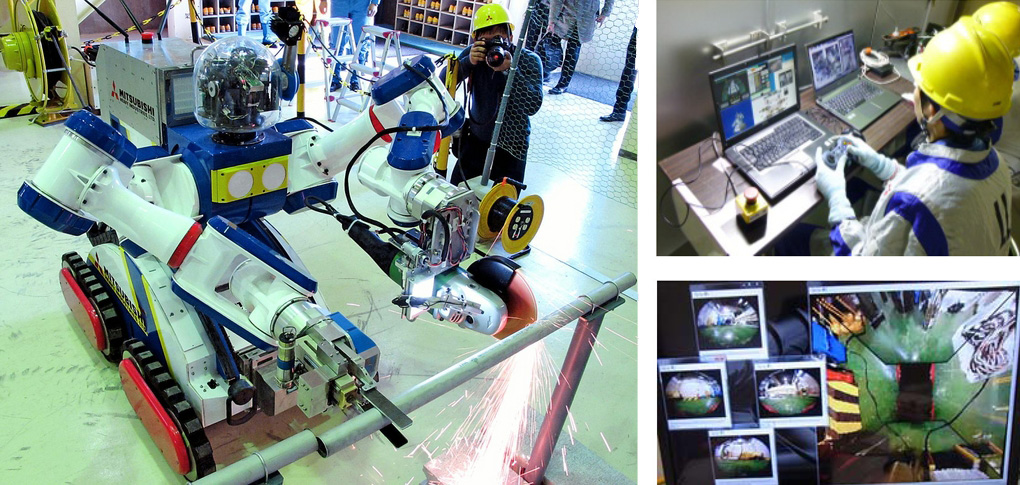
\includegraphics[width=1\textwidth]{meistercomb.jpg}};
%DIFDELCMD < 			\node at (15pt,15pt) {\huge{a}};
%DIFDELCMD < 			\node at (287pt,190pt) {\huge{b}};
%DIFDELCMD < 			\node at (287pt,75pt) {\huge{\textcolor{white}{c}}};
%DIFDELCMD < 	\end{tikzpicture}
%DIFDELCMD < 	%%%
%DIFDELCMD < \caption[Demonstration of MHI MEISTeR at Fukushima Daiichi NPS]{%
{%DIFAUXCMD
\DIFdelFL{Demonstration of the teleoperated MHI MEISTeR robot at Fukushima Daiichi Nuclear Power Station \mbox{%DIFAUXCMD
\cite{MHI-MEISTeR}}%DIFAUXCMD
: a) the robot carrying out a coordinated use of tools task b) operators using video game controllers c) visual feedback for the operator as displayed on the computer screen}}
	%DIFAUXCMD
%DIFDELCMD < \label{FIG:MEISTeR}
%DIFDELCMD < 	\vspace{-10pt}
%DIFDELCMD < \end{figure}
%DIFDELCMD <  %%%
\DIFdelend The robot shown in fig. \ref{FIG:MEISTeR}a is equipped with two arms to cooperatively manipulate tools.\DIFaddbegin \\
\begin{figure}
	\centering
	\begin{tikzpicture}
			\node[above right] (img) at (0,0){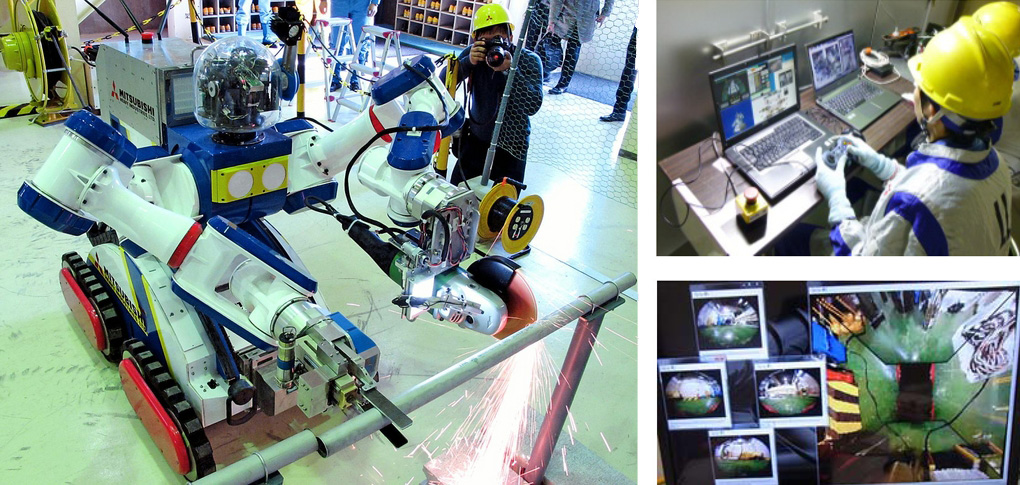
\includegraphics[width=1\textwidth]{meistercomb.jpg}};
			\node at (15pt,15pt) {\huge{a}};
			\node at (287pt,190pt) {\huge{b}};
			\node at (287pt,75pt) {\huge{\textcolor{white}{c}}};
	\end{tikzpicture}
	\caption[Demonstration of MHI MEISTeR at Fukushima Daiichi NPS]{\DIFaddFL{Demonstration of the teleoperated MHI MEISTeR robot at Fukushima Daiichi Nuclear Power Station \mbox{%DIFAUXCMD
\cite{MHI-MEISTeR}}%DIFAUXCMD
: a) the robot carrying out a coordinated use of tools task b) operators using video game controllers c) visual feedback for the operator as displayed on the computer screen}}
	\label{FIG:MEISTeR}
	\vspace{-10pt}
\end{figure}
\DIFaddend The aforementioned input methods have in common that the user is not provided with reactive force-feedback. There is no counteracting force or maximum deflection barrier to limit the possible inputs, thus the user may command arbitrary trajectories. Consider a robotic set-up driven into an obstacle and a user persisting to command motion in the blocked direction. Contact forces and desired velocity become an infinite source of energy. Thus it is indispensable to consider commands that may destabilize the system and/or endanger the environment, especially humans on-site.\\
Concerning safety, a number of collision detection and response strategies exist to make the robot behaviour safe when it comes in contact with a human \cite{Haddadin_14}. These methods work well for slow motion, but for fast and sudden impacts the closed-loop bandwidth of the robots is too slow. The robot's dynamics is then dominated by its effective inertia \cite{Laffranchi_12}. A general solution is to limit the energy stored in the robotic set-up. In an unexpected collision the exchangeable energy is then bounded \cite{Tadele_14}. Empirical studies relate severe injuries of humans to the energetic state of the robot \cite{Wood_71,Yoganandan_96}.\\
Towards a conclusion on closed-loop stability of such a set-up, the major challenge is the unknown dynamic behaviour of the human and the non-restrictive input interfaces. Seen from a control point of view\DIFaddbegin \DIFadd{, }\DIFaddend the human decision making is a "black box", the inputs and outputs are available, but the internal behaviour is unknown. Psychological models based on empirical studies and neural network structures \cite{Peters_15} emulate human behaviour. However, there is no way to guarantee successful modelling of the unpredictable human behaviour. Thus they do not qualify to be the base of a stability proof of the closed-loop behaviour.\\
The objective of this thesis is two-fold: first, a shared control architecture for cooperative object manipulation is designed. \DIFdelbegin \DIFdel{We apply }\DIFdelend \DIFaddbegin \DIFadd{Applying }\DIFaddend the leader-follower paradigm, \DIFdelbegin \DIFdel{where }\DIFdelend a human commands the object motion, while the robots autonomously maintain the coordination (chapter \ref{C:pHS modelling}). \DIFdelbegin \DIFdel{To address stability with the unknown dynamics of human and environment, the }\DIFdelend \DIFaddbegin \DIFadd{The }\DIFaddend controller is passive, i.e. \DIFdelbegin \DIFdel{never generates energy . Second, we propose }\DIFdelend \DIFaddbegin \DIFadd{is asymptotically stable with any environment iff the energy supply is finite. Therefore the second goal is }\DIFaddend an energy shaping approach to cope with an unmodeled human in the loop, who can command arbitrary trajectories \DIFaddbegin \DIFadd{and thus supply infinite energy}\DIFaddend . Bounding the energy in the system ensures closed loop stability and enhances the safety for humans in the environment of the robots (chapter \ref{C:Energy-aware control}).\\
Energy is a major entity in this thesis, a power-consistent formulation allows insights into energy flow and facilitates stability proofs. Thus it is functional to choose an energy-based system description\DIFdelbegin \DIFdel{, the }\DIFdelend \DIFaddbegin \DIFadd{. The }\DIFaddend port-Hamiltonian representation additionally allows a model-based controller design.\\
\textbf{Chapter \DIFdelbegin \DIFdel{2}\DIFdelend \DIFaddbegin \DIFadd{\ref{C:pHS modelling}}\DIFaddend } starts with a general introduction to the port-Hamiltonian framework and details on the description of 3D-mechanical systems. \DIFdelbegin \DIFdel{We compose the }\DIFdelend \DIFaddbegin \DIFadd{By interconnection of virtual mechanical elements two }\DIFaddend model-based \DIFdelbegin \DIFdel{controller of virtual mechanic elements , by interconnection the overall dynamic behaviour is shaped}\DIFdelend \DIFaddbegin \DIFadd{controllers are designed}\DIFaddend .\\
\textbf{Chapter \DIFdelbegin \DIFdel{3}\DIFdelend \DIFaddbegin \DIFadd{\ref{C:Energy-aware control}}\DIFaddend } introduces \DIFaddbegin \DIFadd{an energy tank to limit the energy supply to the controllers designed in chapter 2. An }\DIFaddend adaptive coupling of \DIFaddbegin \DIFadd{user and robots is proposed to shape the energy exchange dependent on the tank level.}\\
\textbf{\DIFadd{Chapter \ref{C:SimulationResults}}} \DIFadd{presents simulation results of the schemes developed in chapter 2 and compares them to known approaches. The effectiveness of }\DIFaddend the \DIFdelbegin \DIFdel{human operator, by relaxing the coupling the The energy-shaping control presented in chapter \ref{C:Energy-aware control} uses adaptive coupling of human and robotic  
}\DIFdelend \DIFaddbegin \DIFadd{energy-bounded trajectory tracking is also verified by simulation.}\\
\textbf{\DIFadd{Chapter \ref{C:Conclusion}}} \DIFadd{draws a brief conclusion and some remarks on future directions are given.
}\DIFaddend 


%To address this uncertainty, passivity-based approaches are widely used \cite{Hirche_12}. Passivity is based on energy considerations, i.e. a system is passive if supplied energy is either stored or dissipated, but never generated in the system. The dissipation leads to asymptotic stability. Another useful property of passive systems is their modularity. The interconnection of a passive system with another passive system is again passive. The connection of a passive system to an unknown system is stable as long as the unknown system can only provide a finite amount of energy \cite{Stramigioli_15}. When a human manipulates a haptic device and her/his motion is subjected to reactive force feedback, closed-loop stability can be concluded because at the frequencies of interest the human muscles are passive \cite{Hogan_89}. For non-reactive user interfaces these assumptions do not hold because the user can issue trajectories with unbounded energy. It is easy to visualize a robotic set-up driven into an obstacle and a user persisting to command motion in the blocked direction. Contact forces and desired velocity become an infinite source of energy. In such a case the control scheme is accountable for limiting the requested energy. The apparent solution of monitoring and terminating energy usage at a certain threshold is impracticable, because actions on the  (unknown) environment require the use of energy, making the choice of this threshold arbitrary. In this thesis a model-based controller is designed to simulate the energetic state of the robotic system, this allows to distinguish between energy appropriately spent on the task and energy driving the system to a potentially harmful state. The latter type is kept bounded by energy shaping control, i.e. dynamically adapting the controller parameters.\\
%For energy being a major entity in this thesis, it is functional to choose a corresponding system description, i.e. the port-Hamiltonian representation.

\section{Problem Statement}

%\textit{You can either state the problem you are trying to solve in the general introduction, providing the transition from the overall picture to your specific approach, or state it in a separate section. Even if you don't use the separate section, writing down in a few sentences why the problem you are trying to solve is actually hard and hasn't been solved before can give you a better idea of how to approach the topic. This can be also merged with the related work part.}\\
\DIFdelbegin %DIFDELCMD < 

%DIFDELCMD < %%%
\DIFdel{A human user controls a team of robots explicitly, there }\DIFdelend \DIFaddbegin \DIFadd{Multiple robots manipulate a common object, the human user guides the formation by hand motion. There }\DIFaddend are two major \DIFdelbegin \DIFdel{problems: How can the operator control the cooperative team efficiently and intuitively and how can we }\DIFdelend \DIFaddbegin \DIFadd{challenges to be considered in this type of human-robot team interaction: $1$) How to address the coordination of the multiple robots in order to let the operator focus on object motion; 2) How to }\DIFaddend achieve stability and safety with the human in the loop\DIFdelbegin \DIFdel{?}\DIFdelend \DIFaddbegin \DIFadd{.}\DIFaddend \\
The \DIFaddbegin \DIFadd{full set-up of human-robot team interaction to analyse and model is shown in figure \ref{FIG:ProblemOverview}.
The }\DIFaddend user does not interact physically with the robots, but is virtually coupled in the manner of a leader-follower scheme\DIFdelbegin \DIFdel{, figure \ref{FIG:ProblemOverview} shows the set-up}\DIFdelend . When cooperatively handling an object, the robots need to preserve a certain formation to avoid dropping or excessive squeezing of the object.
\DIFdelbegin %DIFDELCMD < \begin{figure}[b]
%DIFDELCMD < 			\centering
%DIFDELCMD < 			%%%
%DIF < \psfrag{q1}[Bl][Bl]{\small $\alpha$}
			%DIFDELCMD < 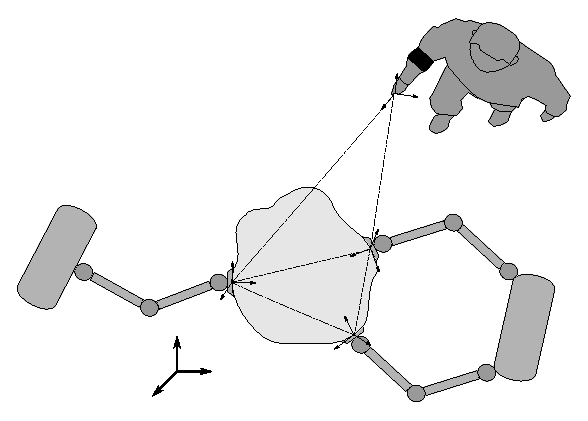
\includegraphics[width=0.4\textwidth]{general_setup.eps}
%DIFDELCMD < 			%%%
%DIFDELCMD < \caption{%
{%DIFAUXCMD
\DIFdelFL{A human user controlling a robotic team by hand motion}}
			%DIFAUXCMD
%DIFDELCMD < \label{FIG:ProblemOverview}
%DIFDELCMD < %%%
\DIFdelendFL 

\DIFdelbeginFL %DIFDELCMD < \end{figure}
%DIFDELCMD <  %%%
\DIFdelend Thus the controller has two tasks, \DIFdelbegin \DIFdel{first, }\DIFdelend \DIFaddbegin \DIFadd{$1$) }\DIFaddend to ensure trajectory following with respect to the human motion (high-level task)\DIFdelbegin \DIFdel{and second, }\DIFdelend \DIFaddbegin \DIFadd{, $2$) }\DIFaddend to generate suitable trajectories for each robot to respect the coordination requirements (low-level task). The control scheme to be designed is thus shared, \DIFdelbegin \DIFdel{for having }\DIFdelend \DIFaddbegin \DIFadd{since it has }\DIFaddend an autonomous part (formation preservation) and a human command part (movement of the formation).\\
\DIFdelbegin %DIFDELCMD < 

%DIFDELCMD < %%%
\DIFdelend In such a shared control set-up the control loop encompasses the human and the environment the robot team interacts with. 
Towards stability and safety the major challenge is the largely unknown dynamics of both human and environment.
Input interfaces that do not restrict the human commands, either by a counteracting force, or maximum deflection, allow for infeasible and/or unsafe trajectories. \DIFdelbegin \DIFdel{In sum no assumptions on possible commands are made, it }\DIFdelend \DIFaddbegin \DIFadd{It }\DIFaddend is the objective of the controller to achieve safe and stable operation for arbitrary inputs.
\DIFaddbegin \begin{figure}[h!]
			\centering
			%DIF > \psfrag{q1}[Bl][Bl]{\small $\alpha$}
			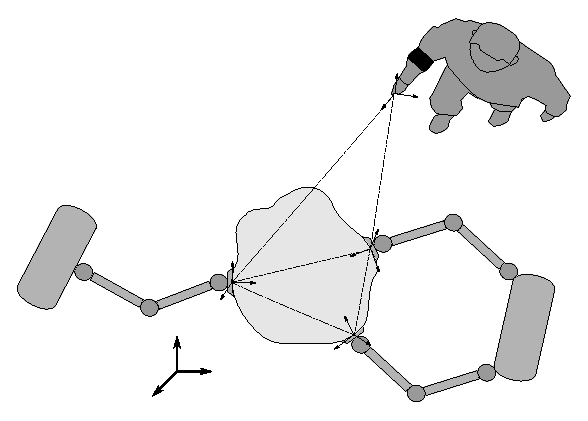
\includegraphics[width=0.4\textwidth]{general_setup.eps}
			\caption{\DIFaddFL{A human user interacting with a robotic team cooperatively grasping and manipulating an object}}
			\label{FIG:ProblemOverview}

\end{figure}
\DIFaddend %With unmodelled dynamics on both sides of the controlled robotic system, the only feasible method to assess stability and safety is monitoring the inputs and outputs of the robots. In this way an estimated state of the system is available to adjust the execution of the commands if necessary. 


\DIFaddbegin \newpage
\DIFaddend \section{Cooperative manipulation and energy regulation control}
A number of classic control schemes for cooperative object manipulation are object-centred and therefore qualify for shared control approaches. They use the so-called \emph{grasp matrix} to relate object and manipulator motion and force distribution \DIFaddbegin \DIFadd{\mbox{%DIFAUXCMD
\cite{CoopManipHandbook}}%DIFAUXCMD
}\DIFaddend . The first to use also the impedance control paradigm \cite{Hogan_84} \DIFaddbegin \DIFadd{in cooperative manipulation tasks }\DIFaddend are Schneider and Cannon \cite{Schneider_92}\DIFdelbegin \DIFdel{, establishing }\DIFdelend \DIFaddbegin \DIFadd{. They establish }\DIFaddend a compliant relation between the desired and the actual object pose. Bonitz and Hsia \cite{Bonitz_96} use an impedance relation between the object and each manipulator. This is essential to ensure stability during contact and non-contact transitions. Both impedance relations are combined in \cite{Caccavale_01,Caccavale_08} and more recent in \cite{Heck_13}. Notably the latter elaborates on (asymptotic) stability of the control scheme with a known environment.\\
\DIFdelbegin \DIFdel{Stability with a wide class of unknown environments }\DIFdelend \DIFaddbegin \DIFadd{The mentioned control schemes employ second-order impedance control to achieve a very dynamic trajectory tracking but are not passive. The cancellation of open-loop dynamics generates possibly unbounded energy. Stramigioli \mbox{%DIFAUXCMD
\cite{Stramigioli_15} }%DIFAUXCMD
points out the effectiveness of passivity when dealing with unknown environments, as for every non-passive controller a passive environment exists that destabilizes the overall system.}\\
\DIFadd{Stability with unknown environments, which can only supply a limited amount of energy, }\DIFaddend is achieved by the \emph{Intrinsically Passive Controller} \cite{Stramigioli_01}\DIFdelbegin \DIFdel{, slightly different }\DIFdelend \DIFaddbegin \DIFadd{. The original version has no dampers in parallel with the springs and thus has a weak dynamic performance.   Different }\DIFaddend implementations on the DLR Hand II \DIFdelbegin \DIFdel{are described in \mbox{%DIFAUXCMD
\cite{Wimboeck_06,Wimboeck_08} }%DIFAUXCMD
}\DIFdelend \DIFaddbegin \DIFadd{\mbox{%DIFAUXCMD
\cite{Wimboeck_06,Wimboeck_08} }%DIFAUXCMD
add the dampers along the springs}\DIFaddend . Instead of using the grasp matrix to describe the kinematic relations of object and manipulators, a virtual structure with a simulated object is introduced. \DIFdelbegin \DIFdel{Thus these schemes are framed by the }\emph{\DIFdel{control by interconnection}} %DIFAUXCMD
\DIFdel{approach \mbox{%DIFAUXCMD
\cite{Ortega_08}  }%DIFAUXCMD
and }\DIFdelend \DIFaddbegin \DIFadd{Virtual structures are a well known tool in }\DIFaddend \emph{formation control} \DIFdelbegin \DIFdel{\mbox{%DIFAUXCMD
\cite{Lawton_03}}%DIFAUXCMD
. Formation control establishes a certain group behaviour for }\DIFdelend \DIFaddbegin \DIFadd{to establish a certain geometric shape of }\DIFaddend several robotic manipulators \DIFdelbegin \DIFdel{to achieve a geometric shape \mbox{%DIFAUXCMD
\cite{VosDiss_15}}%DIFAUXCMD
}\DIFdelend \DIFaddbegin \DIFadd{\mbox{%DIFAUXCMD
\cite{Lawton_03}}%DIFAUXCMD
}\DIFaddend . Virtual springs and dampers are used in \cite{Vos_14} to coordinate the formation driving of a group a wheeled robots. The Intrinsically Passive Controller features a virtual structure of springs, dampers and a mass (the virtual pendant of the common object). Asymptotic stability follows from the passive nature of the (virtual) mechanical elements \cite{Stramigioli_15}. Recently, Sieber et al. \cite{Sieber_15} establish formation control of several manipulators around a common object and study the control options for a human to direct the closed formation.\\
A human operator is easily included in the formation by virtual spring coupling, especially when in a leader-follower scheme \cite{Scheggi_14}. The human leader can be virtually connected to all or some robots \cite{Sieber_15}, a certain point (e.g. the geometric center of the formation) \cite{Wimboeck_06}, or an element of the virtual structure (e.g. the manipulated object) \cite{Stramigioli_01}.\\
The concept of passivity is widely used when including a human in the control loop \cite{Hirche_12}. Passive systems either store or dissipate supplied energy, i.e. they reach an energetic equilibrium, iff the energy supply is finite. Thus the only requirement to achieve stability with a passive robot team is, for the human, to supply only a bounded amount of energy \cite{Stramigioli_15}. To guarantee that only a certain amount of energy is available, an \emph{energy tank} replaces the human to provide energy to the robots. When combined with a proper re-filling strategy the tank concept effectively limits the rate of energy exchange. Known applications of tanks are variable rate haptics \cite{Lee_10} and teleoperation over delayed communication lines \cite{Franken_11}. Re-filling is necessary because performing actions on the environment usually consumes energy, i.e. energy is permanently withdrawn from the system.\\ 
In addition, a tank sourced system can be controlled dependent on its energetic state. The general concept, of actively stabilizing a system at a certain energy level, is usually called \emph{energy shaping control} \cite{Ortega_99}. \DIFaddbegin \DIFadd{The energy stored in a robotic system is also a benchmark for possible injuries when it comes to a collision with a human \mbox{%DIFAUXCMD
\cite{Wood_71,Yoganandan_96}}%DIFAUXCMD
. }\DIFaddend Approaches to maintain a safe level in single robots modify the given reference trajectory \cite{Laffranchi_09}, or adapt the internal behaviour of the robot \cite{Tadele_14}. Very recent, energy shaping \DIFaddbegin \DIFadd{for safety reasons }\DIFaddend is proposed for a robotic team, that is physically coupled to the human \cite{Geravand_16}.\\
The methodology of energy regulation for teleoperated robotic teams is largely unexplored in literature. \DIFdelbegin \DIFdel{Robotic teams carrying out a }\DIFdelend \DIFaddbegin \DIFadd{Neither are there safety evaluations for }\DIFaddend cooperative object manipulation \DIFdelbegin \DIFdel{task can generate high impacts in collisions, due to their higher overall inertia. There are no examinations on safety for this specific task. If we allow arbitrary trajectory commands, even such that potentially supply infinite energy to the robots}\DIFdelend \DIFaddbegin \DIFadd{tasks. Safety concerns are appropriate because of the higher moving inertias (and thus kinetic energy) in such a set-up. If a user interface allows arbitrary trajectories to be commanded, some require infinite energy for the execution}\DIFaddend , then passively controlled robots are not sufficient to conclude stability. To the best of the author's knowledge this problem has not been considered so far.




%____________________________________________________



%_____Kapitel 2_________________________________
\chapter{port-Hamiltonian modelling \DIFaddbegin \DIFadd{in cooperative manipualtion tasks}\DIFaddend }\label{C:pHS modelling}
%The controller is divided into two parts, the local one does the real-time interaction of the manipulators with the object. This part is passive, i.e. the robot along with its local controller has a certain amount of energy, the energy can not increase as long as no power is provided by the environment or the higher-level control part. Therefore the two parts will be called Intrinsically Passive Controller and Supervisor, this scheme was introduced by Stramigioli \cite{Stramigioli_01} as a general framework with application to robotic hands.
In this chapter \DIFdelbegin \DIFdel{we introduce a modelling approach }\DIFdelend \DIFaddbegin \DIFadd{a model }\DIFaddend of the cooperative \DIFaddbegin \DIFadd{manipulation }\DIFaddend system in the port-Hamiltonian framework \DIFdelbegin \DIFdel{. This formulation is based on energy, a major entity in this thesis. Throughout this chapter it will be clear }\DIFdelend \DIFaddbegin \DIFadd{is introduced. The formulation describes the dynamic behaviour based on the total energy stored in the system. This chapter shows }\DIFaddend how energy consistent modelling facilitates control design, allows insights into the flow of energy in the system and provides a ready-made stability proof. The first section \DIFdelbegin \DIFdel{is dedicated to illustrate these advantages }\DIFdelend \DIFaddbegin \DIFadd{\ref{S:energybasedmodelling} illustrates the advantages of energy-based modelling }\DIFaddend in more detail. The general theory of port-Hamiltonian systems is presented in section \ref{S:HSdescription}\DIFdelbegin \DIFdel{and its  generalization for }\DIFdelend \DIFaddbegin \DIFadd{. The extension of the port-Hamiltonian modelling to }\DIFaddend six-dimensional mechanical systems \DIFaddbegin \DIFadd{is provided }\DIFaddend in section \ref{S:3Dspace-modelling}.\DIFdelbegin \DIFdel{An elementary module in mechanical systems are }\DIFdelend \DIFaddbegin \\
\DIFadd{The modelling of the cooperative set-up starts from a }\DIFaddend spring-mass-damper \DIFdelbegin \DIFdel{systems, as they reproduce }\DIFdelend \DIFaddbegin \DIFadd{system. This composition is a common part of complex mechanical systems and reproduces }\DIFaddend a compliant contact\DIFdelbegin \DIFdel{. Their construction }\DIFdelend \DIFaddbegin \DIFadd{, the formulation is derived }\DIFaddend in section \ref{S:springmassdampers}\DIFdelbegin \DIFdel{is an example how the systematic interconnection of the atomic mechanical elements works}\DIFdelend . The counterpart of a compliant contact, namely the \DIFdelbegin \DIFdel{rigid }\DIFdelend \DIFaddbegin \DIFadd{constrained }\DIFaddend contact is treated in section \ref{S:ImposingConstraints}. \DIFdelbegin \DIFdel{Then we have all }\DIFdelend \DIFaddbegin \DIFadd{Contact descriptions and mechanical elements are }\DIFaddend the preliminaries to model a cooperative manipulation set-up. Inspired by the virtual structures to achieve a group behaviour in formation control \cite{Lawton_03}, \DIFdelbegin \DIFdel{we design }\DIFdelend a model-based controller \DIFaddbegin \DIFadd{is designed }\DIFaddend in the last section \ref{S:modelbasedcontrol}.

\section{Energy-based modelling and control}\DIFaddbegin \label{S:energybasedmodelling}
\DIFaddend Every physical process involves energy and especially energy transfers or transformations. Energy \DIFdelbegin \DIFdel{is a very general concept in physical systems, it }\DIFdelend allows for a consistent description across different physical domains. Even within the mechanical domain there are two forms of energy (kinetic, potential)\DIFdelbegin \DIFdel{, e. g. acceleration can be viewed as a transition from potential to kinetic energy. }\DIFdelend \DIFaddbegin \DIFadd{. }\DIFaddend Energetic relations do not only define static relations between physical systems but also \DIFdelbegin \DIFdel{their }\DIFdelend \DIFaddbegin \DIFadd{the }\DIFaddend dynamic behaviour, described by the transient exchange of energy \cite{Ortega_01}. The modelling of a complex physical system can therefore be accomplished by an interconnection of simple subsystems, defined by an energy function. \DIFdelbegin \DIFdel{We can combine }\DIFdelend \DIFaddbegin \DIFadd{A proper combination of }\DIFaddend such physical elements \DIFdelbegin \DIFdel{to achieve }\DIFdelend \DIFaddbegin \DIFadd{achieves }\DIFaddend a desired dynamic behaviour and thereby \DIFdelbegin \DIFdel{define }\DIFdelend \DIFaddbegin \DIFadd{defines }\DIFaddend a model-based controller on energetic level.  In contrast to this, control is traditionally handled from a signal processing viewpoint. Starting from a reference input, an output signal is generated to reduce some error signal. Control design on the energetic level allows to build a model-based controller in a physically meaningful way. An energetically consistent control scheme visualizes the flow of energy in the system (e.g. energy supplied by an operator \DIFaddbegin \DIFadd{and }\DIFaddend distributed to the robots) and \DIFdelbegin \DIFdel{is intrinsically passive}\DIFdelend \DIFaddbegin \DIFadd{enables }\emph{\DIFadd{passivity-based control}} \DIFadd{design}\DIFaddend . Considering the energy balance of the controlled system and explicitly performing control by shaping the energy is the foundation of passivity based control. \DIFdelbegin \DIFdel{Passive controlled robots are appropriate when dealing }\DIFdelend \DIFaddbegin \DIFadd{Passivity-based control in robotics is appropriate when considering interaction }\DIFaddend with unknown environments (see also chapter \ref{C:Energy-aware control} and \cite{Stramigioli_15}).\\
Another motivation for control design on energy level is safety in physical human-robot interaction or co-working. The kinetic energy stored in the robotic system is intimately connected with the risk of severe injuries of a human. Assume a human \DIFdelbegin \DIFdel{explicitly }\DIFdelend controlling a robotic team \DIFdelbegin \DIFdel{, by her/his commands s/he supplies }\DIFdelend \DIFaddbegin \DIFadd{and as a result supplying }\DIFaddend energy to the controller\DIFdelbegin \DIFdel{and the controller }\DIFdelend \DIFaddbegin \DIFadd{, which }\DIFaddend distributes the energy to the robots. Because of its formulation on the energy level, the controller is aware of the energetic state of the system and \DIFdelbegin \DIFdel{can adapt }\DIFdelend \DIFaddbegin \DIFadd{adapts }\DIFaddend its behaviour to keep the energy bounded (see chapter \ref{C:Energy-aware control}).\\
For the energy-consistent modelling of mechanical systems two approaches are known:  the \DIFdelbegin \DIFdel{Lagrangian and the Hamiltonian. In recent years }\DIFdelend \DIFaddbegin \emph{\DIFadd{Lagrangian}} \DIFadd{and the }\emph{\DIFadd{Hamiltonian}} \DIFadd{approach. Since }\DIFaddend a combination of the Hamiltonian description and port-based interconnection \DIFdelbegin \DIFdel{was developed }\DIFdelend \DIFaddbegin \DIFadd{is developed in recent years}\DIFaddend , we refer to port-Hamiltonian modelling. It allows to describe complex physical systems based on the interconnection of simpler subsystems, represented in a convenient input-state-output formulation, which has the structure of a (non-linear) state space formulation. The Hamiltonian function of the interconnected system sums up the total energy stored in the subsystem and is a \DIFdelbegin \DIFdel{Lyapunov }\DIFdelend \DIFaddbegin \emph{\DIFadd{Lyapunov}} \DIFaddend candidate function, facilitating stability proofs.

%\section{Formation control for cooperative manipulation}
%A more general perspective on cooperative manipulation is opened from a formation control viewpoint. A common assumption for cooperative manipulation is rigid connection between the common object and the manipulators \cite{CoopManipHandbook}, leading to a geometric set-up described by a \emph{grasp matrix}. Based on a particular choice of a weighted pseudoinverse of this matrix \cite{Walker_91},\cite{Erhart_15} forces are distributed from the object to the manipulators, an approach with little physical interpretation according to \cite{Wimboeck_08}. The intuition of formation control is to establish a certain group behaviour for several robotic manipulators to achieve a geometric shape \cite{VosDiss_15}. One of the three types of formation control described in \cite{Lawton_03} is virtual structures between mobile robots. Virtual springs and dampers are used in \cite{Vos_14} to coordinate the formation driving of a group a wheeled robots. Recently, Sieber et al. \cite{Sieber_15} establish formation control of several manipulators around a common object and study the control options for a human to direct the closed formation. The dynamics of the handled object is not considered in the control scheme, however we often deal with large and heavy objects with non-negligible inertia. In the virtual structure of Stramigioli's \emph{Intrinsically Passive Controller} each the robots is connected with a virtual spring to a common, virtual object.

\section{port-Hamiltonian description of mechanical systems}\label{S:HSdescription}
For the derivation of the port-Hamiltonian description of a mechanical system we start from the classical \emph{Euler-Lagrange} equations of motion
\begin{equation}
\frac{d}{dt}\left(\frac{\partial \mathcal{L}}{\partial \dot{\f{q}}}\right) - \frac{\partial \mathcal{L}}{\partial \f{q}} = G(\f{q})\f{u},
\end{equation}
where $\f{q} \in \mathbb{R}^k$ is the vector of generalized configuration coordinates of the system. The \emph{Lagrangian} $\mathcal{L} = V_\g{K} - V_\g{P}$ equals the difference between the kinetic co-energy $V_\g{K}$ and the potential energy $V_\g{P}$. The kinetic co-energy is explicitly given as $V_\g{K} = \frac{1}{2} \dot{\f{q}}^T M(\f{q}) \dot{\f{q}}$, with a symmetric, positive definite inertia matrix $M(\f{q}) \in \mathbb{R}^{k \times k}$. The generalized forces $\f{u} \in \mathbb{R}^m$ act on the system with an input matrix $G(\f{q}) \in \mathbb{R}^{k \times m}$. We define the generalized \emph{momenta} for every Lagrangian $\f{p} := \frac{\partial \mathcal{L}}{\partial \dot{\f{q}}}$ and obtain $\f{p} = M(\f{q})\dot{\f{q}}$.
\DIFdelbegin \DIFdel{Introducing the }\DIFdelend \DIFaddbegin \DIFadd{The }\DIFaddend \emph{Hamiltonian} (energy) function 
\DIFdelbegin \DIFdel{$\mathcal{H}(\f{q},\f{p}) = \f{p}^T\dot{\f{q}} - \mathcal{L}(\f{q},\dot{\f{q}})$ we can }\DIFdelend \DIFaddbegin \begin{equation}\DIFadd{\label{EQ:Hamiltonian}
\mathcal{H}(\f{q},\f{p}) = \underbrace{\f{p}^T\dot{\f{q}}}_{2V_{\g{K}}} - \underbrace{\mathcal{L}(\f{q},\dot{\f{q}})}_{V_{\g{K}}-V_{\g{P}}}
}\end{equation} \DIFadd{allows to }\DIFaddend rewrite the Euler-Lagrange equation in form of the classical Hamiltonian equations of a mechanical system \begin{eqnarray}\label{EQ:mechanicalPHS}
	\begin{aligned}
	& \dot{\f{q}} = \frac{\partial \mathcal{H}}{\partial \f{p}}(\f{q},\f{p})\\
	& \dot{\f{p}} = -\frac{\partial \mathcal{H}}{\partial \f{q}}(\f{q},\f{p}) + G(\f{q})\f{u}
	\end{aligned}
\end{eqnarray}
\DIFdelbegin \DIFdel{The Hamiltonian describes the }\DIFdelend \DIFaddbegin \DIFadd{Equation (\ref{EQ:Hamiltonian}) that the Hamiltonian is the sum of kinetic and potential energy, i.e. the }\DIFaddend total energy stored in the system \cite{vanderSchaft_06}\DIFdelbegin \DIFdel{, thus the }\DIFdelend \DIFaddbegin \DIFadd{. The }\DIFaddend energy balance is
\begin{equation}\DIFaddbegin \label{EQ:PHSenergystorage}
	\DIFaddend \frac{d}{dt}\mathcal{H} = \frac{\partial^T \mathcal{H}}{\partial \f{q}}(\f{q},\f{p})\dot{\f{q}} + \frac{\partial^T \mathcal{H}}{\partial p}(\f{q},\f{p})\dot{\f{p}} = \f{u}^TG^T(\f{q})\dot{\f{q}} = \f{u}^T\f{y}
\end{equation}
Hamiltonian systems are energy conservative, i.e. the \DIFdelbegin \DIFdel{energy supplied through the port }\DIFdelend \DIFaddbegin \DIFadd{supplied energy }\DIFaddend is stored in the system. In \DIFdelbegin \DIFdel{the upper equation }\DIFdelend \DIFaddbegin \DIFadd{equation \ref{EQ:PHSenergystorage} }\DIFaddend a new output $\f{y}=G^T(\f{q})\dot{\f{q}}$ is introduced. Clearly the product $\f{y}^T\f{u}$ is the exchanged power and \DIFdelbegin \DIFdel{we call }\DIFdelend the pair $(\f{u},\f{y})$ \DIFaddbegin \DIFadd{is called }\DIFaddend a \emph{power port}. 
The general equations of a port-Hamiltonian system are
\begin{eqnarray}
\begin{aligned}
	& \dot{\f{q}} = \frac{\partial \mathcal{H}}{\partial \f{p}}				(\f{q},\f{p})\\
	& \dot{\f{p}} = -\frac{\partial \mathcal{H}}{\partial \f{q}}				(\f{q},\f{p})+G(\f{q})\f{u} \\ 
	&\f{y} = G^T(\f{q})\frac{\partial \mathcal{H}}{\partial 				\f{p}}(\f{q},\f{p})
\end{aligned}	
\end{eqnarray}
Port-Hamiltonian systems are suitable to describe a variety of physical systems including mechanical, electrical, thermal and hydraulic elements, see \cite{duindam2009geoplexbook} for an overview. The common ground \DIFdelbegin \DIFdel{is that }\DIFdelend \DIFaddbegin \DIFadd{across the physical domains is the Hamiltonian energy function and }\DIFaddend inputs and outputs \DIFdelbegin \DIFdel{are dual quantities , this motivates the more general input-output concept of flows }\DIFdelend \DIFaddbegin \DIFadd{being dual quantities (e.g. velocity-force, current-voltage, heat flow-temperature change). To emphasize this inherent relation, inputs }\DIFaddend $\f{u}$ \DIFdelbegin \DIFdel{and efforts }\DIFdelend \DIFaddbegin \DIFadd{are called }\emph{\DIFadd{flows}}  \DIFadd{and outputs }\DIFaddend $\f{y}$ \DIFdelbegin \DIFdel{forming the port variables $(\f{u},\f{y})$. }\DIFdelend \DIFaddbegin \DIFadd{are called }\emph{\DIFadd{efforts}}\DIFadd{. A more formal definition of ports, efforts and flows can be found in the next subsection \ref{SS:PHSinterconnection}. The general appearance of a port-Hamiltonian system in the form of a (non-linear) state-space formulation becomes apparent in the following example.}\DIFaddend \\
\textbf{Example 2.1:}\\
Consider a simple one-dimensional spring-mass system described by the equation $ m\ddot{x} = -kx +F $ and shown in figure \ref{FIG:springmass}. The parameters $ m,k,F $ denote the mass, stiffness and external force acting on the mass respectively. A state space formulation of the system is
\begin{figure}[b!]
	\centering
	\small
	\def\svgwidth{0.5\columnwidth}
	%LaTeX with PSTricks extensions
%%Creator: 0.91_64bit
%%Please note this file requires PSTricks extensions
\psset{xunit=.5pt,yunit=.5pt,runit=.5pt}
\begin{pspicture}(744.09448819,1052.36220472)
{
\newrgbcolor{curcolor}{1 1 1}
\pscustom[linestyle=none,fillstyle=solid,fillcolor=curcolor]
{
\newpath
\moveto(433.9839592,679.23058241)
\curveto(433.9839592,660.64698979)(418.9189808,645.5820114)(400.33538818,645.5820114)
\curveto(381.75179557,645.5820114)(366.68681717,660.64698979)(366.68681717,679.23058241)
\curveto(366.68681717,697.81417503)(381.75179557,712.87915342)(400.33538818,712.87915342)
\curveto(418.9189808,712.87915342)(433.9839592,697.81417503)(433.9839592,679.23058241)
\closepath
}
}
{
\newrgbcolor{curcolor}{0 0 0}
\pscustom[linewidth=1.5,linecolor=curcolor]
{
\newpath
\moveto(433.9839592,679.23058241)
\curveto(433.9839592,660.64698979)(418.9189808,645.5820114)(400.33538818,645.5820114)
\curveto(381.75179557,645.5820114)(366.68681717,660.64698979)(366.68681717,679.23058241)
\curveto(366.68681717,697.81417503)(381.75179557,712.87915342)(400.33538818,712.87915342)
\curveto(418.9189808,712.87915342)(433.9839592,697.81417503)(433.9839592,679.23058241)
\closepath
}
}
{
\newrgbcolor{curcolor}{0 0 0}
\pscustom[linewidth=1.5,linecolor=curcolor]
{
\newpath
\moveto(144.85715,678.81484472)
\lineto(158.74845,678.81484472)
\curveto(158.74845,678.81484472)(163.37889,697.33658472)(181.90063,697.33658472)
\curveto(191.1615,697.33658472)(195.79193,682.59527472)(195.79193,678.81484472)
\curveto(195.79193,674.18441472)(195.79193,660.37820472)(186.53106,660.29311472)
\curveto(181.90083,660.25051472)(177.27019,669.38803472)(177.27019,678.81484472)
\curveto(177.27019,688.07571472)(181.90063,697.33658472)(195.79193,697.33658472)
}
}
{
\newrgbcolor{curcolor}{0 0 0}
\pscustom[linewidth=1.5,linecolor=curcolor]
{
\newpath
\moveto(195.79193,697.33658472)
\curveto(209.68324,697.33658472)(214.31367,682.59527472)(214.31367,678.81484472)
\curveto(214.31367,674.18441472)(214.31367,660.37820472)(205.0528,660.29311472)
\curveto(200.42256,660.25051472)(195.79193,669.38803472)(195.79193,678.81484472)
\curveto(195.79193,688.07571472)(200.42237,697.33658472)(214.31367,697.33658472)
}
}
{
\newrgbcolor{curcolor}{0 0 0}
\pscustom[linewidth=1.5,linecolor=curcolor]
{
\newpath
\moveto(214.31367,697.33658472)
\curveto(228.20498,697.33658472)(232.83541,682.59527472)(232.83541,678.81484472)
\curveto(232.83541,674.18441472)(232.83541,660.37820472)(223.57454,660.29311472)
\curveto(218.9443,660.25051472)(214.31367,669.38803472)(214.31367,678.81484472)
\curveto(214.31367,688.07571472)(218.94411,697.33658472)(232.83541,697.33658472)
}
}
{
\newrgbcolor{curcolor}{0 0 0}
\pscustom[linewidth=1.5,linecolor=curcolor]
{
\newpath
\moveto(232.83541,697.33658472)
\curveto(246.72672,697.33658472)(251.35715,682.59527472)(251.35715,678.81484472)
\curveto(251.35715,674.18441472)(251.35715,660.37820472)(242.09628,660.29311472)
\curveto(237.46604,660.25051472)(232.83541,669.38803472)(232.83541,678.81484472)
\curveto(232.83541,688.07571472)(237.46585,697.33658472)(251.35715,697.33658472)
}
}
{
\newrgbcolor{curcolor}{0 0 0}
\pscustom[linewidth=1.5,linecolor=curcolor]
{
\newpath
\moveto(251.35715,697.33658472)
\curveto(265.24845,697.33658472)(269.87889,682.59527472)(269.87889,678.81484472)
\curveto(269.87889,674.18441472)(269.87889,660.37820472)(260.61802,660.29311472)
\curveto(255.98778,660.25051472)(251.35715,669.38803472)(251.35715,678.81484472)
\curveto(251.35715,688.07571472)(255.98758,697.33658472)(269.87889,697.33658472)
}
}
{
\newrgbcolor{curcolor}{0 0 0}
\pscustom[linewidth=1.5,linecolor=curcolor]
{
\newpath
\moveto(269.87889,697.33658472)
\curveto(283.77019,697.33658472)(288.40063,682.59527472)(288.40063,678.81484472)
\curveto(288.40063,674.18441472)(288.40063,660.37820472)(279.13976,660.29311472)
\curveto(274.50952,660.25051472)(269.87889,669.38803472)(269.87889,678.81484472)
\curveto(269.87889,688.07571472)(274.50932,697.33658472)(288.40063,697.33658472)
}
}
{
\newrgbcolor{curcolor}{0 0 0}
\pscustom[linewidth=1.5,linecolor=curcolor]
{
\newpath
\moveto(288.40063,697.33658472)
\curveto(302.29193,697.33658472)(306.92237,682.59527472)(306.92237,678.81484472)
\curveto(306.92237,674.18441472)(306.92237,660.37820472)(297.6615,660.29311472)
\curveto(293.03126,660.25051472)(288.40063,669.38803472)(288.40063,678.81484472)
\curveto(288.40063,688.07571472)(293.03106,697.33658472)(306.92237,697.33658472)
}
}
{
\newrgbcolor{curcolor}{0 0 0}
\pscustom[linewidth=1.5,linecolor=curcolor]
{
\newpath
\moveto(357.85715,678.81484472)
\lineto(343.96585,678.81484472)
\curveto(343.96585,678.81484472)(339.33541,697.33658472)(320.81367,697.33658472)
\curveto(311.5528,697.33658472)(306.92237,688.07571472)(306.92237,678.81484472)
\curveto(306.92237,674.18441472)(306.92237,660.29311472)(316.18324,660.29311472)
\curveto(320.81367,660.29311472)(325.44411,669.38803472)(325.44411,678.81484472)
\curveto(325.44411,688.07571472)(320.81367,697.33658472)(306.92237,697.33658472)
}
}
{
\newrgbcolor{curcolor}{0 0 0}
\pscustom[linewidth=1.5,linecolor=curcolor]
{
\newpath
\moveto(144.82296,644.79884472)
\lineto(144.82296,714.99972472)
}
}
{
\newrgbcolor{curcolor}{1 1 1}
\pscustom[linestyle=none,fillstyle=solid,fillcolor=curcolor]
{
\newpath
\moveto(365.97257495,678.80568617)
\curveto(365.97257495,676.63421108)(364.21224658,674.8738827)(362.04077148,674.8738827)
\curveto(359.86929639,674.8738827)(358.10896802,676.63421108)(358.10896802,678.80568617)
\curveto(358.10896802,680.97716126)(359.86929639,682.73748963)(362.04077148,682.73748963)
\curveto(364.21224658,682.73748963)(365.97257495,680.97716126)(365.97257495,678.80568617)
\closepath
}
}
{
\newrgbcolor{curcolor}{0 0 0}
\pscustom[linewidth=1.5,linecolor=curcolor]
{
\newpath
\moveto(365.97257495,678.80568617)
\curveto(365.97257495,676.63421108)(364.21224658,674.8738827)(362.04077148,674.8738827)
\curveto(359.86929639,674.8738827)(358.10896802,676.63421108)(358.10896802,678.80568617)
\curveto(358.10896802,680.97716126)(359.86929639,682.73748963)(362.04077148,682.73748963)
\curveto(364.21224658,682.73748963)(365.97257495,680.97716126)(365.97257495,678.80568617)
\closepath
}
}
{
\newrgbcolor{curcolor}{0 0 0}
\pscustom[linewidth=1.5,linecolor=curcolor]
{
\newpath
\moveto(137,715.00000472)
\lineto(145,708.00000472)
}
}
{
\newrgbcolor{curcolor}{0 0 0}
\pscustom[linewidth=1.5,linecolor=curcolor]
{
\newpath
\moveto(137,708.00000472)
\lineto(145,701.00000472)
}
}
{
\newrgbcolor{curcolor}{0 0 0}
\pscustom[linewidth=1.5,linecolor=curcolor]
{
\newpath
\moveto(137,701.00000472)
\lineto(145,694.00000472)
}
}
{
\newrgbcolor{curcolor}{0 0 0}
\pscustom[linewidth=1.5,linecolor=curcolor]
{
\newpath
\moveto(137,694.00000472)
\lineto(145,687.00000472)
}
}
{
\newrgbcolor{curcolor}{0 0 0}
\pscustom[linewidth=1.5,linecolor=curcolor]
{
\newpath
\moveto(137,687.00000472)
\lineto(145,680.00000472)
}
}
{
\newrgbcolor{curcolor}{0 0 0}
\pscustom[linewidth=1.5,linecolor=curcolor]
{
\newpath
\moveto(137,680.00000472)
\lineto(145,673.00000472)
}
}
{
\newrgbcolor{curcolor}{0 0 0}
\pscustom[linewidth=1.5,linecolor=curcolor]
{
\newpath
\moveto(137,673.00000472)
\lineto(145,666.00000472)
}
}
{
\newrgbcolor{curcolor}{0 0 0}
\pscustom[linewidth=1.5,linecolor=curcolor]
{
\newpath
\moveto(137,666.00000472)
\lineto(145,659.00000472)
}
}
{
\newrgbcolor{curcolor}{0 0 0}
\pscustom[linewidth=1.5,linecolor=curcolor]
{
\newpath
\moveto(137,659.00000472)
\lineto(145,652.00000472)
}
}
{
\newrgbcolor{curcolor}{0 0 0}
\pscustom[linewidth=1.5,linecolor=curcolor]
{
\newpath
\moveto(137,652.00000472)
\lineto(145,645.00000472)
}
}
{
\newrgbcolor{curcolor}{0 0 0}
\pscustom[linestyle=none,fillstyle=solid,fillcolor=curcolor]
{
\newpath
\moveto(442.23874,683.17562062)
\lineto(434,680.65661472)
\lineto(442.23874,678.13760882)
\closepath
}
}
{
\newrgbcolor{curcolor}{0 0 0}
\pscustom[linewidth=1.68894935,linecolor=curcolor]
{
\newpath
\moveto(442.15625,680.81250472)
\lineto(473.5343,680.81250472)
}
}
{
\newrgbcolor{curcolor}{0 0 0}
\pscustom[linestyle=none,fillstyle=solid,fillcolor=curcolor]
{
\newpath
\moveto(481.57217407,678.58635634)
\curveto(481.57217407,677.95565972)(481.32599894,677.43075738)(480.83364868,677.0116493)
\curveto(480.34129842,676.59661024)(479.69636027,676.35043511)(478.89883423,676.27312391)
\lineto(478.89883423,674.06365126)
\lineto(478.17861938,674.06365126)
\lineto(478.17861938,676.24260634)
\curveto(477.64151001,676.24667535)(477.13695272,676.29753798)(476.66494751,676.39519423)
\curveto(476.1929423,676.49691949)(475.78400675,676.62712782)(475.43814087,676.78581923)
\lineto(475.43814087,677.99431532)
\lineto(475.53579712,677.99431532)
\curveto(475.61310832,677.93734917)(475.75145467,677.85393446)(475.95083618,677.74407118)
\curveto(476.15021769,677.63827691)(476.34349569,677.55079318)(476.53067017,677.48162001)
\curveto(476.74225871,677.40430881)(476.98843384,677.33106662)(477.26919556,677.26189345)
\curveto(477.55402629,677.19678928)(477.85716756,677.15813368)(478.17861938,677.14592665)
\lineto(478.17861938,679.78874891)
\curveto(478.01585897,679.821301)(477.86530558,679.85181858)(477.72695923,679.88030165)
\curveto(477.58861287,679.91285373)(477.46043905,679.94540581)(477.34243774,679.9779579)
\curveto(476.67918905,680.14478733)(476.20311483,680.39503147)(475.91421509,680.72869032)
\curveto(475.62531535,681.06641818)(475.48086548,681.48145725)(475.48086548,681.97380751)
\curveto(475.48086548,682.57602105)(475.71686808,683.08464735)(476.18887329,683.49968641)
\curveto(476.66494751,683.91472548)(477.32819621,684.1568316)(478.17861938,684.22600477)
\lineto(478.17861938,685.88616102)
\lineto(478.89883423,685.88616102)
\lineto(478.89883423,684.2382118)
\curveto(479.30980428,684.23007378)(479.73094686,684.18124566)(480.16226196,684.09172743)
\curveto(480.59357707,684.0022092)(480.95571899,683.89844943)(481.24868774,683.78044813)
\lineto(481.24868774,682.58415907)
\lineto(481.16323853,682.58415907)
\curveto(480.85806274,682.77133355)(480.53864543,682.93612847)(480.20498657,683.07854384)
\curveto(479.87539673,683.22502821)(479.44001261,683.31658095)(478.89883423,683.35320204)
\lineto(478.89883423,680.7225868)
\curveto(479.02090454,680.70224175)(479.15314738,680.67375868)(479.29556274,680.63713759)
\curveto(479.43797811,680.6045855)(479.56208293,680.57813693)(479.6678772,680.55779188)
\curveto(480.27415975,680.42758355)(480.74209595,680.20378798)(481.07168579,679.88640516)
\curveto(481.40534465,679.56902235)(481.57217407,679.13567274)(481.57217407,678.58635634)
\closepath
\moveto(478.17861938,680.82634657)
\lineto(478.17861938,683.34709852)
\curveto(477.74323527,683.31454644)(477.37702433,683.19451063)(477.07998657,682.9869911)
\curveto(476.78294881,682.78354058)(476.63442993,682.49870985)(476.63442993,682.13249891)
\curveto(476.63442993,681.76221897)(476.74429321,681.48349175)(476.96401978,681.29631727)
\curveto(477.18374634,681.10914279)(477.58861287,680.95248589)(478.17861938,680.82634657)
\closepath
\moveto(480.41860962,678.42766493)
\curveto(480.41860962,678.81015191)(480.29857381,679.08887912)(480.0585022,679.26384657)
\curveto(479.82249959,679.44288303)(479.4359436,679.58326389)(478.89883423,679.68498915)
\lineto(478.89883423,677.15813368)
\curveto(479.38711548,677.2069618)(479.76146444,677.33106662)(480.0218811,677.53044813)
\curveto(480.28636678,677.72982964)(480.41860962,678.02890191)(480.41860962,678.42766493)
\closepath
}
}
{
\newrgbcolor{curcolor}{0 0 0}
\pscustom[linestyle=none,fillstyle=solid,fillcolor=curcolor]
{
\newpath
\moveto(489.24429321,673.87444227)
\lineto(488.32876587,673.87444227)
\curveto(487.600413,673.87444227)(487.00837199,674.07789279)(486.55264282,674.48479384)
\curveto(486.10098267,674.88762587)(485.87515259,675.47152886)(485.87515259,676.23650282)
\lineto(485.87515259,677.14592665)
\curveto(485.87515259,677.83358941)(485.70628866,678.37069878)(485.36856079,678.75725477)
\curveto(485.03083293,679.14787977)(484.5140686,679.34319227)(483.81826782,679.34319227)
\lineto(483.50698853,679.34319227)
\lineto(483.50698853,680.29534071)
\lineto(483.81826782,680.29534071)
\curveto(484.5140686,680.29534071)(485.03083293,680.48861871)(485.36856079,680.8751747)
\curveto(485.70628866,681.2657997)(485.87515259,681.80494358)(485.87515259,682.49260634)
\lineto(485.87515259,683.40203016)
\curveto(485.87515259,684.16700412)(486.10098267,684.75090712)(486.55264282,685.15373915)
\curveto(487.00837199,685.56064019)(487.600413,685.76409071)(488.32876587,685.76409071)
\lineto(489.24429321,685.76409071)
\lineto(489.24429321,684.92180555)
\lineto(488.54849243,684.92180555)
\curveto(487.99510701,684.92180555)(487.59227498,684.79363173)(487.33999634,684.53728407)
\curveto(487.0917867,684.28093641)(486.96768188,683.86793186)(486.96768188,683.2982704)
\lineto(486.96768188,682.23015516)
\curveto(486.96768188,681.66456272)(486.81102498,681.1884885)(486.49771118,680.80193251)
\curveto(486.18439738,680.41944553)(485.74901326,680.11630425)(485.19155884,679.89250868)
\lineto(485.19155884,679.7460243)
\curveto(485.74901326,679.52222873)(486.18439738,679.21705295)(486.49771118,678.83049696)
\curveto(486.81102498,678.44800998)(486.96768188,677.97397027)(486.96768188,677.40837782)
\lineto(486.96768188,676.34026259)
\curveto(486.96768188,675.77060113)(487.0917867,675.35759657)(487.33999634,675.10124891)
\curveto(487.59227498,674.84490126)(487.99510701,674.71672743)(488.54849243,674.71672743)
\lineto(489.24429321,674.71672743)
\lineto(489.24429321,673.87444227)
\closepath
}
}
{
\newrgbcolor{curcolor}{0 0 0}
\pscustom[linestyle=none,fillstyle=solid,fillcolor=curcolor]
{
\newpath
\moveto(497.41079712,684.28093641)
\lineto(492.81484985,684.28093641)
\lineto(492.81484985,681.71745985)
\lineto(496.76382446,681.71745985)
\lineto(496.76382446,680.6432411)
\lineto(492.81484985,680.6432411)
\lineto(492.81484985,676.2670204)
\lineto(491.60635376,676.2670204)
\lineto(491.60635376,685.35515516)
\lineto(497.41079712,685.35515516)
\lineto(497.41079712,684.28093641)
\closepath
}
}
{
\newrgbcolor{curcolor}{0 0 0}
\pscustom[linestyle=none,fillstyle=solid,fillcolor=curcolor]
{
\newpath
\moveto(504.44204712,679.34319227)
\lineto(504.13076782,679.34319227)
\curveto(503.43496704,679.34319227)(502.91820272,679.14787977)(502.58047485,678.75725477)
\curveto(502.24274699,678.37069878)(502.07388306,677.83358941)(502.07388306,677.14592665)
\lineto(502.07388306,676.23650282)
\curveto(502.07388306,675.47152886)(501.84601847,674.88762587)(501.39028931,674.48479384)
\curveto(500.93862915,674.07789279)(500.34862264,673.87444227)(499.62026978,673.87444227)
\lineto(498.70474243,673.87444227)
\lineto(498.70474243,674.71672743)
\lineto(499.40054321,674.71672743)
\curveto(499.95392863,674.71672743)(500.35472616,674.84490126)(500.60293579,675.10124891)
\curveto(500.85521444,675.35759657)(500.98135376,675.77060113)(500.98135376,676.34026259)
\lineto(500.98135376,677.40837782)
\curveto(500.98135376,677.97397027)(501.13801066,678.44800998)(501.45132446,678.83049696)
\curveto(501.76463826,679.21705295)(502.20002238,679.52222873)(502.75747681,679.7460243)
\lineto(502.75747681,679.89250868)
\curveto(502.20002238,680.11630425)(501.76463826,680.41944553)(501.45132446,680.80193251)
\curveto(501.13801066,681.1884885)(500.98135376,681.66456272)(500.98135376,682.23015516)
\lineto(500.98135376,683.2982704)
\curveto(500.98135376,683.86793186)(500.85521444,684.28093641)(500.60293579,684.53728407)
\curveto(500.35472616,684.79363173)(499.95392863,684.92180555)(499.40054321,684.92180555)
\lineto(498.70474243,684.92180555)
\lineto(498.70474243,685.76409071)
\lineto(499.62026978,685.76409071)
\curveto(500.34862264,685.76409071)(500.93862915,685.56064019)(501.39028931,685.15373915)
\curveto(501.84601847,684.75090712)(502.07388306,684.16700412)(502.07388306,683.40203016)
\lineto(502.07388306,682.49260634)
\curveto(502.07388306,681.80494358)(502.24274699,681.2657997)(502.58047485,680.8751747)
\curveto(502.91820272,680.48861871)(503.43496704,680.29534071)(504.13076782,680.29534071)
\lineto(504.44204712,680.29534071)
\lineto(504.44204712,679.34319227)
\closepath
}
}
{
\newrgbcolor{curcolor}{0 0 0}
\pscustom[linestyle=none,fillstyle=solid,fillcolor=curcolor]
{
\newpath
\moveto(512.57803345,678.58635634)
\curveto(512.57803345,677.95565972)(512.33185832,677.43075738)(511.83950806,677.0116493)
\curveto(511.3471578,676.59661024)(510.70221965,676.35043511)(509.9046936,676.27312391)
\lineto(509.9046936,674.06365126)
\lineto(509.18447876,674.06365126)
\lineto(509.18447876,676.24260634)
\curveto(508.64736938,676.24667535)(508.14281209,676.29753798)(507.67080688,676.39519423)
\curveto(507.19880168,676.49691949)(506.78986613,676.62712782)(506.44400024,676.78581923)
\lineto(506.44400024,677.99431532)
\lineto(506.54165649,677.99431532)
\curveto(506.61896769,677.93734917)(506.75731405,677.85393446)(506.95669556,677.74407118)
\curveto(507.15607707,677.63827691)(507.34935506,677.55079318)(507.53652954,677.48162001)
\curveto(507.74811808,677.40430881)(507.99429321,677.33106662)(508.27505493,677.26189345)
\curveto(508.55988566,677.19678928)(508.86302694,677.15813368)(509.18447876,677.14592665)
\lineto(509.18447876,679.78874891)
\curveto(509.02171834,679.821301)(508.87116496,679.85181858)(508.7328186,679.88030165)
\curveto(508.59447225,679.91285373)(508.46629842,679.94540581)(508.34829712,679.9779579)
\curveto(507.68504842,680.14478733)(507.2089742,680.39503147)(506.92007446,680.72869032)
\curveto(506.63117472,681.06641818)(506.48672485,681.48145725)(506.48672485,681.97380751)
\curveto(506.48672485,682.57602105)(506.72272746,683.08464735)(507.19473267,683.49968641)
\curveto(507.67080688,683.91472548)(508.33405558,684.1568316)(509.18447876,684.22600477)
\lineto(509.18447876,685.88616102)
\lineto(509.9046936,685.88616102)
\lineto(509.9046936,684.2382118)
\curveto(510.31566366,684.23007378)(510.73680623,684.18124566)(511.16812134,684.09172743)
\curveto(511.59943644,684.0022092)(511.96157837,683.89844943)(512.25454712,683.78044813)
\lineto(512.25454712,682.58415907)
\lineto(512.1690979,682.58415907)
\curveto(511.86392212,682.77133355)(511.5445048,682.93612847)(511.21084595,683.07854384)
\curveto(510.8812561,683.22502821)(510.44587199,683.31658095)(509.9046936,683.35320204)
\lineto(509.9046936,680.7225868)
\curveto(510.02676392,680.70224175)(510.15900675,680.67375868)(510.30142212,680.63713759)
\curveto(510.44383748,680.6045855)(510.5679423,680.57813693)(510.67373657,680.55779188)
\curveto(511.28001912,680.42758355)(511.74795532,680.20378798)(512.07754517,679.88640516)
\curveto(512.41120402,679.56902235)(512.57803345,679.13567274)(512.57803345,678.58635634)
\closepath
\moveto(509.18447876,680.82634657)
\lineto(509.18447876,683.34709852)
\curveto(508.74909465,683.31454644)(508.38288371,683.19451063)(508.08584595,682.9869911)
\curveto(507.78880819,682.78354058)(507.64028931,682.49870985)(507.64028931,682.13249891)
\curveto(507.64028931,681.76221897)(507.75015259,681.48349175)(507.96987915,681.29631727)
\curveto(508.18960571,681.10914279)(508.59447225,680.95248589)(509.18447876,680.82634657)
\closepath
\moveto(511.42446899,678.42766493)
\curveto(511.42446899,678.81015191)(511.30443319,679.08887912)(511.06436157,679.26384657)
\curveto(510.82835897,679.44288303)(510.44180298,679.58326389)(509.9046936,679.68498915)
\lineto(509.9046936,677.15813368)
\curveto(510.39297485,677.2069618)(510.76732381,677.33106662)(511.02774048,677.53044813)
\curveto(511.29222616,677.72982964)(511.42446899,678.02890191)(511.42446899,678.42766493)
\closepath
}
}
{
\newrgbcolor{curcolor}{0 0 0}
\pscustom[linestyle=none,fillstyle=solid,fillcolor=curcolor]
{
\newpath
\moveto(398.98104858,676.38429945)
\curveto(398.98104858,675.75360284)(398.73487345,675.22870049)(398.24252319,674.80959242)
\curveto(397.75017293,674.39455336)(397.10523478,674.14837823)(396.30770874,674.07106703)
\lineto(396.30770874,671.86159437)
\lineto(395.5874939,671.86159437)
\lineto(395.5874939,674.04054945)
\curveto(395.05038452,674.04461846)(394.54582723,674.09548109)(394.07382202,674.19313734)
\curveto(393.60181681,674.2948626)(393.19288127,674.42507094)(392.84701538,674.58376234)
\lineto(392.84701538,675.79225844)
\lineto(392.94467163,675.79225844)
\curveto(393.02198283,675.73529229)(393.16032918,675.65187758)(393.35971069,675.54201429)
\curveto(393.5590922,675.43622002)(393.7523702,675.3487363)(393.93954468,675.27956312)
\curveto(394.15113322,675.20225192)(394.39730835,675.12900974)(394.67807007,675.05983656)
\curveto(394.9629008,674.99473239)(395.26604207,674.95607679)(395.5874939,674.94386976)
\lineto(395.5874939,677.58669203)
\curveto(395.42473348,677.61924411)(395.27418009,677.64976169)(395.13583374,677.67824476)
\curveto(394.99748739,677.71079685)(394.86931356,677.74334893)(394.75131226,677.77590101)
\curveto(394.08806356,677.94273044)(393.61198934,678.19297458)(393.3230896,678.52663344)
\curveto(393.03418986,678.8643613)(392.88973999,679.27940036)(392.88973999,679.77175062)
\curveto(392.88973999,680.37396416)(393.12574259,680.88259047)(393.5977478,681.29762953)
\curveto(394.07382202,681.71266859)(394.73707072,681.95477471)(395.5874939,682.02394789)
\lineto(395.5874939,683.68410414)
\lineto(396.30770874,683.68410414)
\lineto(396.30770874,682.03615492)
\curveto(396.71867879,682.0280169)(397.13982137,681.97918877)(397.57113647,681.88967054)
\curveto(398.00245158,681.80015232)(398.36459351,681.69639255)(398.65756226,681.57839125)
\lineto(398.65756226,680.38210219)
\lineto(398.57211304,680.38210219)
\curveto(398.26693726,680.56927666)(397.94751994,680.73407159)(397.61386108,680.87648695)
\curveto(397.28427124,681.02297133)(396.84888713,681.11452406)(396.30770874,681.15114515)
\lineto(396.30770874,678.52052992)
\curveto(396.42977905,678.50018487)(396.56202189,678.47170179)(396.70443726,678.4350807)
\curveto(396.84685262,678.40252862)(396.97095744,678.37608005)(397.07675171,678.355735)
\curveto(397.68303426,678.22552666)(398.15097046,678.00173109)(398.4805603,677.68434828)
\curveto(398.81421916,677.36696547)(398.98104858,676.93361586)(398.98104858,676.38429945)
\closepath
\moveto(395.5874939,678.62428969)
\lineto(395.5874939,681.14504164)
\curveto(395.15210978,681.11248956)(394.78589884,680.99245375)(394.48886108,680.78493422)
\curveto(394.19182332,680.5814837)(394.04330444,680.29665297)(394.04330444,679.93044203)
\curveto(394.04330444,679.56016208)(394.15316772,679.28143487)(394.37289429,679.09426039)
\curveto(394.59262085,678.90708591)(394.99748739,678.75042901)(395.5874939,678.62428969)
\closepath
\moveto(397.82748413,676.22560804)
\curveto(397.82748413,676.60809502)(397.70744832,676.88682224)(397.46737671,677.06178969)
\curveto(397.2313741,677.24082614)(396.84481812,677.381207)(396.30770874,677.48293226)
\lineto(396.30770874,674.95607679)
\curveto(396.79598999,675.00490492)(397.17033895,675.12900974)(397.43075562,675.32839125)
\curveto(397.69524129,675.52777276)(397.82748413,675.82684502)(397.82748413,676.22560804)
\closepath
}
}
{
\newrgbcolor{curcolor}{0 0 0}
\pscustom[linestyle=none,fillstyle=solid,fillcolor=curcolor]
{
\newpath
\moveto(406.65316772,671.67238539)
\lineto(405.73764038,671.67238539)
\curveto(405.00928752,671.67238539)(404.4172465,671.87583591)(403.96151733,672.28273695)
\curveto(403.50985718,672.68556898)(403.2840271,673.26947198)(403.2840271,674.03444594)
\lineto(403.2840271,674.94386976)
\curveto(403.2840271,675.63153252)(403.11516317,676.1686419)(402.7774353,676.55519789)
\curveto(402.43970744,676.94582289)(401.92294312,677.14113539)(401.22714233,677.14113539)
\lineto(400.91586304,677.14113539)
\lineto(400.91586304,678.09328383)
\lineto(401.22714233,678.09328383)
\curveto(401.92294312,678.09328383)(402.43970744,678.28656182)(402.7774353,678.67311781)
\curveto(403.11516317,679.06374281)(403.2840271,679.60288669)(403.2840271,680.29054945)
\lineto(403.2840271,681.19997328)
\curveto(403.2840271,681.96494724)(403.50985718,682.54885023)(403.96151733,682.95168226)
\curveto(404.4172465,683.35858331)(405.00928752,683.56203383)(405.73764038,683.56203383)
\lineto(406.65316772,683.56203383)
\lineto(406.65316772,682.71974867)
\lineto(405.95736694,682.71974867)
\curveto(405.40398153,682.71974867)(405.0011495,682.59157484)(404.74887085,682.33522719)
\curveto(404.50066121,682.07887953)(404.3765564,681.66587497)(404.3765564,681.09621351)
\lineto(404.3765564,680.02809828)
\curveto(404.3765564,679.46250583)(404.2198995,678.98643161)(403.90658569,678.59987562)
\curveto(403.59327189,678.21738864)(403.15788778,677.91424737)(402.60043335,677.69045179)
\lineto(402.60043335,677.54396742)
\curveto(403.15788778,677.32017185)(403.59327189,677.01499607)(403.90658569,676.62844008)
\curveto(404.2198995,676.2459531)(404.3765564,675.77191338)(404.3765564,675.20632094)
\lineto(404.3765564,674.1382057)
\curveto(404.3765564,673.56854424)(404.50066121,673.15553969)(404.74887085,672.89919203)
\curveto(405.0011495,672.64284437)(405.40398153,672.51467054)(405.95736694,672.51467054)
\lineto(406.65316772,672.51467054)
\lineto(406.65316772,671.67238539)
\closepath
}
}
{
\newrgbcolor{curcolor}{0 0 0}
\pscustom[linestyle=none,fillstyle=solid,fillcolor=curcolor]
{
\newpath
\moveto(418.87240601,674.06496351)
\lineto(417.72494507,674.06496351)
\lineto(417.72494507,677.94679945)
\curveto(417.72494507,678.2397682)(417.71070353,678.52256442)(417.68222046,678.79518812)
\curveto(417.6578064,679.06781182)(417.60287476,679.28550388)(417.51742554,679.44826429)
\curveto(417.4238383,679.62323174)(417.28956095,679.75547458)(417.11459351,679.84499281)
\curveto(416.93962606,679.93451104)(416.68734741,679.97927015)(416.35775757,679.97927015)
\curveto(416.03630575,679.97927015)(415.71485392,679.89788995)(415.3934021,679.73512953)
\curveto(415.07195028,679.57643812)(414.75049845,679.3729876)(414.42904663,679.12477797)
\curveto(414.44125366,679.03119073)(414.45142619,678.92132745)(414.45956421,678.79518812)
\curveto(414.46770223,678.67311781)(414.47177124,678.5510475)(414.47177124,678.42897719)
\lineto(414.47177124,674.06496351)
\lineto(413.3243103,674.06496351)
\lineto(413.3243103,677.94679945)
\curveto(413.3243103,678.24790622)(413.31006877,678.53273695)(413.28158569,678.80129164)
\curveto(413.25717163,679.07391534)(413.20223999,679.29160739)(413.11679077,679.45436781)
\curveto(413.02320353,679.62933526)(412.88892619,679.75954359)(412.71395874,679.84499281)
\curveto(412.53899129,679.93451104)(412.28671265,679.97927015)(411.9571228,679.97927015)
\curveto(411.643809,679.97927015)(411.32846069,679.90195896)(411.01107788,679.74733656)
\curveto(410.69776408,679.59271416)(410.38445028,679.39536716)(410.07113647,679.15529554)
\lineto(410.07113647,674.06496351)
\lineto(408.92367554,674.06496351)
\lineto(408.92367554,680.88259047)
\lineto(410.07113647,680.88259047)
\lineto(410.07113647,680.12575453)
\curveto(410.42920939,680.42279229)(410.7852478,680.65472588)(411.13925171,680.82155531)
\curveto(411.49732463,680.98838474)(411.8777771,681.07179945)(412.28060913,681.07179945)
\curveto(412.74447632,681.07179945)(413.13713582,680.9741432)(413.45858765,680.7788307)
\curveto(413.78410848,680.5835182)(414.0262146,680.31292901)(414.18490601,679.96706312)
\curveto(414.64877319,680.35768812)(415.07195028,680.63844984)(415.45443726,680.80934828)
\curveto(415.83692424,680.98431573)(416.24585978,681.07179945)(416.6812439,681.07179945)
\curveto(417.42994181,681.07179945)(417.98129272,680.84393487)(418.33529663,680.3882057)
\curveto(418.69336955,679.93654554)(418.87240601,679.30381442)(418.87240601,678.49001234)
\lineto(418.87240601,674.06496351)
\closepath
}
}
{
\newrgbcolor{curcolor}{0 0 0}
\pscustom[linestyle=none,fillstyle=solid,fillcolor=curcolor]
{
\newpath
\moveto(426.83139038,677.14113539)
\lineto(426.52011108,677.14113539)
\curveto(425.8243103,677.14113539)(425.30754598,676.94582289)(424.96981812,676.55519789)
\curveto(424.63209025,676.1686419)(424.46322632,675.63153252)(424.46322632,674.94386976)
\lineto(424.46322632,674.03444594)
\curveto(424.46322632,673.26947198)(424.23536174,672.68556898)(423.77963257,672.28273695)
\curveto(423.32797241,671.87583591)(422.7379659,671.67238539)(422.00961304,671.67238539)
\lineto(421.09408569,671.67238539)
\lineto(421.09408569,672.51467054)
\lineto(421.78988647,672.51467054)
\curveto(422.34327189,672.51467054)(422.74406942,672.64284437)(422.99227905,672.89919203)
\curveto(423.2445577,673.15553969)(423.37069702,673.56854424)(423.37069702,674.1382057)
\lineto(423.37069702,675.20632094)
\curveto(423.37069702,675.77191338)(423.52735392,676.2459531)(423.84066772,676.62844008)
\curveto(424.15398153,677.01499607)(424.58936564,677.32017185)(425.14682007,677.54396742)
\lineto(425.14682007,677.69045179)
\curveto(424.58936564,677.91424737)(424.15398153,678.21738864)(423.84066772,678.59987562)
\curveto(423.52735392,678.98643161)(423.37069702,679.46250583)(423.37069702,680.02809828)
\lineto(423.37069702,681.09621351)
\curveto(423.37069702,681.66587497)(423.2445577,682.07887953)(422.99227905,682.33522719)
\curveto(422.74406942,682.59157484)(422.34327189,682.71974867)(421.78988647,682.71974867)
\lineto(421.09408569,682.71974867)
\lineto(421.09408569,683.56203383)
\lineto(422.00961304,683.56203383)
\curveto(422.7379659,683.56203383)(423.32797241,683.35858331)(423.77963257,682.95168226)
\curveto(424.23536174,682.54885023)(424.46322632,681.96494724)(424.46322632,681.19997328)
\lineto(424.46322632,680.29054945)
\curveto(424.46322632,679.60288669)(424.63209025,679.06374281)(424.96981812,678.67311781)
\curveto(425.30754598,678.28656182)(425.8243103,678.09328383)(426.52011108,678.09328383)
\lineto(426.83139038,678.09328383)
\lineto(426.83139038,677.14113539)
\closepath
}
}
{
\newrgbcolor{curcolor}{0 0 0}
\pscustom[linestyle=none,fillstyle=solid,fillcolor=curcolor]
{
\newpath
\moveto(434.96737671,676.38429945)
\curveto(434.96737671,675.75360284)(434.72120158,675.22870049)(434.22885132,674.80959242)
\curveto(433.73650106,674.39455336)(433.09156291,674.14837823)(432.29403687,674.07106703)
\lineto(432.29403687,671.86159437)
\lineto(431.57382202,671.86159437)
\lineto(431.57382202,674.04054945)
\curveto(431.03671265,674.04461846)(430.53215535,674.09548109)(430.06015015,674.19313734)
\curveto(429.58814494,674.2948626)(429.17920939,674.42507094)(428.83334351,674.58376234)
\lineto(428.83334351,675.79225844)
\lineto(428.93099976,675.79225844)
\curveto(429.00831095,675.73529229)(429.14665731,675.65187758)(429.34603882,675.54201429)
\curveto(429.54542033,675.43622002)(429.73869832,675.3487363)(429.9258728,675.27956312)
\curveto(430.13746134,675.20225192)(430.38363647,675.12900974)(430.66439819,675.05983656)
\curveto(430.94922892,674.99473239)(431.2523702,674.95607679)(431.57382202,674.94386976)
\lineto(431.57382202,677.58669203)
\curveto(431.4110616,677.61924411)(431.26050822,677.64976169)(431.12216187,677.67824476)
\curveto(430.98381551,677.71079685)(430.85564168,677.74334893)(430.73764038,677.77590101)
\curveto(430.07439168,677.94273044)(429.59831746,678.19297458)(429.30941772,678.52663344)
\curveto(429.02051799,678.8643613)(428.87606812,679.27940036)(428.87606812,679.77175062)
\curveto(428.87606812,680.37396416)(429.11207072,680.88259047)(429.58407593,681.29762953)
\curveto(430.06015015,681.71266859)(430.72339884,681.95477471)(431.57382202,682.02394789)
\lineto(431.57382202,683.68410414)
\lineto(432.29403687,683.68410414)
\lineto(432.29403687,682.03615492)
\curveto(432.70500692,682.0280169)(433.1261495,681.97918877)(433.5574646,681.88967054)
\curveto(433.9887797,681.80015232)(434.35092163,681.69639255)(434.64389038,681.57839125)
\lineto(434.64389038,680.38210219)
\lineto(434.55844116,680.38210219)
\curveto(434.25326538,680.56927666)(433.93384806,680.73407159)(433.60018921,680.87648695)
\curveto(433.27059937,681.02297133)(432.83521525,681.11452406)(432.29403687,681.15114515)
\lineto(432.29403687,678.52052992)
\curveto(432.41610718,678.50018487)(432.54835002,678.47170179)(432.69076538,678.4350807)
\curveto(432.83318075,678.40252862)(432.95728556,678.37608005)(433.06307983,678.355735)
\curveto(433.66936239,678.22552666)(434.13729858,678.00173109)(434.46688843,677.68434828)
\curveto(434.80054728,677.36696547)(434.96737671,676.93361586)(434.96737671,676.38429945)
\closepath
\moveto(431.57382202,678.62428969)
\lineto(431.57382202,681.14504164)
\curveto(431.13843791,681.11248956)(430.77222697,680.99245375)(430.47518921,680.78493422)
\curveto(430.17815145,680.5814837)(430.02963257,680.29665297)(430.02963257,679.93044203)
\curveto(430.02963257,679.56016208)(430.13949585,679.28143487)(430.35922241,679.09426039)
\curveto(430.57894897,678.90708591)(430.98381551,678.75042901)(431.57382202,678.62428969)
\closepath
\moveto(433.81381226,676.22560804)
\curveto(433.81381226,676.60809502)(433.69377645,676.88682224)(433.45370483,677.06178969)
\curveto(433.21770223,677.24082614)(432.83114624,677.381207)(432.29403687,677.48293226)
\lineto(432.29403687,674.95607679)
\curveto(432.78231812,675.00490492)(433.15666707,675.12900974)(433.41708374,675.32839125)
\curveto(433.68156942,675.52777276)(433.81381226,675.82684502)(433.81381226,676.22560804)
\closepath
}
}
{
\newrgbcolor{curcolor}{0 0 0}
\pscustom[linestyle=none,fillstyle=solid,fillcolor=curcolor]
{
\newpath
\moveto(210.79014587,709.9718849)
\curveto(210.79014587,709.34118829)(210.54397074,708.81628594)(210.05162048,708.39717787)
\curveto(209.55927022,707.98213881)(208.91433207,707.73596368)(208.11680603,707.65865248)
\lineto(208.11680603,705.44917982)
\lineto(207.39659119,705.44917982)
\lineto(207.39659119,707.6281349)
\curveto(206.85948181,707.63220391)(206.35492452,707.68306654)(205.88291931,707.78072279)
\curveto(205.4109141,707.88244805)(205.00197856,708.01265638)(204.65611267,708.17134779)
\lineto(204.65611267,709.37984388)
\lineto(204.75376892,709.37984388)
\curveto(204.83108012,709.32287774)(204.96942647,709.23946303)(205.16880798,709.12959974)
\curveto(205.36818949,709.02380547)(205.56146749,708.93632175)(205.74864197,708.86714857)
\curveto(205.96023051,708.78983737)(206.20640564,708.71659519)(206.48716736,708.64742201)
\curveto(206.77199809,708.58231784)(207.07513936,708.54366224)(207.39659119,708.53145521)
\lineto(207.39659119,711.17427748)
\curveto(207.23383077,711.20682956)(207.08327738,711.23734714)(206.94493103,711.26583021)
\curveto(206.80658468,711.2983823)(206.67841085,711.33093438)(206.56040955,711.36348646)
\curveto(205.89716085,711.53031589)(205.42108663,711.78056003)(205.13218689,712.11421888)
\curveto(204.84328715,712.45194675)(204.69883728,712.86698581)(204.69883728,713.35933607)
\curveto(204.69883728,713.96154961)(204.93483988,714.47017592)(205.40684509,714.88521498)
\curveto(205.88291931,715.30025404)(206.54616801,715.54236016)(207.39659119,715.61153334)
\lineto(207.39659119,717.27168959)
\lineto(208.11680603,717.27168959)
\lineto(208.11680603,715.62374037)
\curveto(208.52777608,715.61560235)(208.94891866,715.56677422)(209.38023376,715.47725599)
\curveto(209.81154887,715.38773776)(210.1736908,715.283978)(210.46665955,715.1659767)
\lineto(210.46665955,713.96968763)
\lineto(210.38121033,713.96968763)
\curveto(210.07603455,714.15686211)(209.75661723,714.32165704)(209.42295837,714.4640724)
\curveto(209.09336853,714.61055678)(208.65798442,714.70210951)(208.11680603,714.7387306)
\lineto(208.11680603,712.10811537)
\curveto(208.23887634,712.08777032)(208.37111918,712.05928724)(208.51353455,712.02266615)
\curveto(208.65594991,711.99011407)(208.78005473,711.9636655)(208.885849,711.94332045)
\curveto(209.49213155,711.81311211)(209.96006775,711.58931654)(210.28965759,711.27193373)
\curveto(210.62331645,710.95455092)(210.79014587,710.52120131)(210.79014587,709.9718849)
\closepath
\moveto(207.39659119,712.21187513)
\lineto(207.39659119,714.73262709)
\curveto(206.96120707,714.700075)(206.59499613,714.5800392)(206.29795837,714.37251967)
\curveto(206.00092061,714.16906914)(205.85240173,713.88423842)(205.85240173,713.51802748)
\curveto(205.85240173,713.14774753)(205.96226501,712.86902032)(206.18199158,712.68184584)
\curveto(206.40171814,712.49467136)(206.80658468,712.33801446)(207.39659119,712.21187513)
\closepath
\moveto(209.63658142,709.81319349)
\curveto(209.63658142,710.19568047)(209.51654561,710.47440769)(209.276474,710.64937513)
\curveto(209.04047139,710.82841159)(208.65391541,710.96879245)(208.11680603,711.07051771)
\lineto(208.11680603,708.54366224)
\curveto(208.60508728,708.59249037)(208.97943624,708.71659519)(209.23985291,708.9159767)
\curveto(209.50433858,709.11535821)(209.63658142,709.41443047)(209.63658142,709.81319349)
\closepath
}
}
{
\newrgbcolor{curcolor}{0 0 0}
\pscustom[linestyle=none,fillstyle=solid,fillcolor=curcolor]
{
\newpath
\moveto(218.46226501,705.25997084)
\lineto(217.54673767,705.25997084)
\curveto(216.81838481,705.25997084)(216.22634379,705.46342136)(215.77061462,705.8703224)
\curveto(215.31895447,706.27315443)(215.09312439,706.85705743)(215.09312439,707.62203138)
\lineto(215.09312439,708.53145521)
\curveto(215.09312439,709.21911797)(214.92426046,709.75622735)(214.58653259,710.14278334)
\curveto(214.24880473,710.53340834)(213.73204041,710.72872084)(213.03623962,710.72872084)
\lineto(212.72496033,710.72872084)
\lineto(212.72496033,711.68086928)
\lineto(213.03623962,711.68086928)
\curveto(213.73204041,711.68086928)(214.24880473,711.87414727)(214.58653259,712.26070326)
\curveto(214.92426046,712.65132826)(215.09312439,713.19047214)(215.09312439,713.8781349)
\lineto(215.09312439,714.78755873)
\curveto(215.09312439,715.55253269)(215.31895447,716.13643568)(215.77061462,716.53926771)
\curveto(216.22634379,716.94616875)(216.81838481,717.14961928)(217.54673767,717.14961928)
\lineto(218.46226501,717.14961928)
\lineto(218.46226501,716.30733412)
\lineto(217.76646423,716.30733412)
\curveto(217.21307882,716.30733412)(216.81024679,716.17916029)(216.55796814,715.92281263)
\curveto(216.3097585,715.66646498)(216.18565369,715.25346042)(216.18565369,714.68379896)
\lineto(216.18565369,713.61568373)
\curveto(216.18565369,713.05009128)(216.02899679,712.57401706)(215.71568298,712.18746107)
\curveto(215.40236918,711.80497409)(214.96698507,711.50183282)(214.40953064,711.27803724)
\lineto(214.40953064,711.13155287)
\curveto(214.96698507,710.9077573)(215.40236918,710.60258151)(215.71568298,710.21602553)
\curveto(216.02899679,709.83353855)(216.18565369,709.35949883)(216.18565369,708.79390638)
\lineto(216.18565369,707.72579115)
\curveto(216.18565369,707.15612969)(216.3097585,706.74312513)(216.55796814,706.48677748)
\curveto(216.81024679,706.23042982)(217.21307882,706.10225599)(217.76646423,706.10225599)
\lineto(218.46226501,706.10225599)
\lineto(218.46226501,705.25997084)
\closepath
}
}
{
\newrgbcolor{curcolor}{0 0 0}
\pscustom[linestyle=none,fillstyle=solid,fillcolor=curcolor]
{
\newpath
\moveto(226.92173767,707.65254896)
\lineto(225.4080658,707.65254896)
\lineto(222.6736908,710.6371681)
\lineto(221.92906189,709.92916029)
\lineto(221.92906189,707.65254896)
\lineto(220.78160095,707.65254896)
\lineto(220.78160095,717.14961928)
\lineto(221.92906189,717.14961928)
\lineto(221.92906189,711.05831068)
\lineto(225.24327087,714.47017592)
\lineto(226.68980408,714.47017592)
\lineto(223.52207947,711.32076185)
\lineto(226.92173767,707.65254896)
\closepath
}
}
{
\newrgbcolor{curcolor}{0 0 0}
\pscustom[linestyle=none,fillstyle=solid,fillcolor=curcolor]
{
\newpath
\moveto(233.87974548,710.72872084)
\lineto(233.56846619,710.72872084)
\curveto(232.87266541,710.72872084)(232.35590108,710.53340834)(232.01817322,710.14278334)
\curveto(231.68044535,709.75622735)(231.51158142,709.21911797)(231.51158142,708.53145521)
\lineto(231.51158142,707.62203138)
\curveto(231.51158142,706.85705743)(231.28371684,706.27315443)(230.82798767,705.8703224)
\curveto(230.37632751,705.46342136)(229.786321,705.25997084)(229.05796814,705.25997084)
\lineto(228.1424408,705.25997084)
\lineto(228.1424408,706.10225599)
\lineto(228.83824158,706.10225599)
\curveto(229.39162699,706.10225599)(229.79242452,706.23042982)(230.04063416,706.48677748)
\curveto(230.2929128,706.74312513)(230.41905212,707.15612969)(230.41905212,707.72579115)
\lineto(230.41905212,708.79390638)
\curveto(230.41905212,709.35949883)(230.57570903,709.83353855)(230.88902283,710.21602553)
\curveto(231.20233663,710.60258151)(231.63772074,710.9077573)(232.19517517,711.13155287)
\lineto(232.19517517,711.27803724)
\curveto(231.63772074,711.50183282)(231.20233663,711.80497409)(230.88902283,712.18746107)
\curveto(230.57570903,712.57401706)(230.41905212,713.05009128)(230.41905212,713.61568373)
\lineto(230.41905212,714.68379896)
\curveto(230.41905212,715.25346042)(230.2929128,715.66646498)(230.04063416,715.92281263)
\curveto(229.79242452,716.17916029)(229.39162699,716.30733412)(228.83824158,716.30733412)
\lineto(228.1424408,716.30733412)
\lineto(228.1424408,717.14961928)
\lineto(229.05796814,717.14961928)
\curveto(229.786321,717.14961928)(230.37632751,716.94616875)(230.82798767,716.53926771)
\curveto(231.28371684,716.13643568)(231.51158142,715.55253269)(231.51158142,714.78755873)
\lineto(231.51158142,713.8781349)
\curveto(231.51158142,713.19047214)(231.68044535,712.65132826)(232.01817322,712.26070326)
\curveto(232.35590108,711.87414727)(232.87266541,711.68086928)(233.56846619,711.68086928)
\lineto(233.87974548,711.68086928)
\lineto(233.87974548,710.72872084)
\closepath
}
}
{
\newrgbcolor{curcolor}{0 0 0}
\pscustom[linestyle=none,fillstyle=solid,fillcolor=curcolor]
{
\newpath
\moveto(242.01573181,709.9718849)
\curveto(242.01573181,709.34118829)(241.76955668,708.81628594)(241.27720642,708.39717787)
\curveto(240.78485616,707.98213881)(240.13991801,707.73596368)(239.34239197,707.65865248)
\lineto(239.34239197,705.44917982)
\lineto(238.62217712,705.44917982)
\lineto(238.62217712,707.6281349)
\curveto(238.08506775,707.63220391)(237.58051046,707.68306654)(237.10850525,707.78072279)
\curveto(236.63650004,707.88244805)(236.22756449,708.01265638)(235.88169861,708.17134779)
\lineto(235.88169861,709.37984388)
\lineto(235.97935486,709.37984388)
\curveto(236.05666606,709.32287774)(236.19501241,709.23946303)(236.39439392,709.12959974)
\curveto(236.59377543,709.02380547)(236.78705343,708.93632175)(236.97422791,708.86714857)
\curveto(237.18581645,708.78983737)(237.43199158,708.71659519)(237.7127533,708.64742201)
\curveto(237.99758403,708.58231784)(238.3007253,708.54366224)(238.62217712,708.53145521)
\lineto(238.62217712,711.17427748)
\curveto(238.45941671,711.20682956)(238.30886332,711.23734714)(238.17051697,711.26583021)
\curveto(238.03217061,711.2983823)(237.90399679,711.33093438)(237.78599548,711.36348646)
\curveto(237.12274679,711.53031589)(236.64667257,711.78056003)(236.35777283,712.11421888)
\curveto(236.06887309,712.45194675)(235.92442322,712.86698581)(235.92442322,713.35933607)
\curveto(235.92442322,713.96154961)(236.16042582,714.47017592)(236.63243103,714.88521498)
\curveto(237.10850525,715.30025404)(237.77175395,715.54236016)(238.62217712,715.61153334)
\lineto(238.62217712,717.27168959)
\lineto(239.34239197,717.27168959)
\lineto(239.34239197,715.62374037)
\curveto(239.75336202,715.61560235)(240.1745046,715.56677422)(240.6058197,715.47725599)
\curveto(241.03713481,715.38773776)(241.39927673,715.283978)(241.69224548,715.1659767)
\lineto(241.69224548,713.96968763)
\lineto(241.60679626,713.96968763)
\curveto(241.30162048,714.15686211)(240.98220317,714.32165704)(240.64854431,714.4640724)
\curveto(240.31895447,714.61055678)(239.88357035,714.70210951)(239.34239197,714.7387306)
\lineto(239.34239197,712.10811537)
\curveto(239.46446228,712.08777032)(239.59670512,712.05928724)(239.73912048,712.02266615)
\curveto(239.88153585,711.99011407)(240.00564067,711.9636655)(240.11143494,711.94332045)
\curveto(240.71771749,711.81311211)(241.18565369,711.58931654)(241.51524353,711.27193373)
\curveto(241.84890238,710.95455092)(242.01573181,710.52120131)(242.01573181,709.9718849)
\closepath
\moveto(238.62217712,712.21187513)
\lineto(238.62217712,714.73262709)
\curveto(238.18679301,714.700075)(237.82058207,714.5800392)(237.52354431,714.37251967)
\curveto(237.22650655,714.16906914)(237.07798767,713.88423842)(237.07798767,713.51802748)
\curveto(237.07798767,713.14774753)(237.18785095,712.86902032)(237.40757751,712.68184584)
\curveto(237.62730408,712.49467136)(238.03217061,712.33801446)(238.62217712,712.21187513)
\closepath
\moveto(240.86216736,709.81319349)
\curveto(240.86216736,710.19568047)(240.74213155,710.47440769)(240.50205994,710.64937513)
\curveto(240.26605733,710.82841159)(239.87950134,710.96879245)(239.34239197,711.07051771)
\lineto(239.34239197,708.54366224)
\curveto(239.83067322,708.59249037)(240.20502218,708.71659519)(240.46543884,708.9159767)
\curveto(240.72992452,709.11535821)(240.86216736,709.41443047)(240.86216736,709.81319349)
\closepath
}
}
\end{pspicture}

	\caption[Spring-mass example]{Spring-mass example}
	%\vspace{-20pt}
	\label{FIG:springmass}
\end{figure}
\begin{equation}
	\begin{pmatrix}\dot{x} \\ \ddot{x}\end{pmatrix} =
	\begin{pmatrix}0 & 1 \\ -\frac{k}{m} & 0\end{pmatrix}
	\begin{pmatrix}x \\ \dot{x}\end{pmatrix} + 
	\begin{pmatrix}0 \\ 1\end{pmatrix}\frac{F}{m}
\end{equation}
In the Hamiltonian approach the system is described based on the energy functions, being $ V_\g{P}(q) = \frac{1}{2}kq^2 $ for the spring and $ V_\g{K}(p) = \frac{1}{2m}p^2 $ for the mass. The total energy is thus the Hamiltonian $\mathcal{H}(q,p) = V_\g{K} + V_\g{P}$ The state variables are thus replaced by the energy states, the \emph{configuration} $q=x$ accounting for the spring and the \emph{momentum} $p=m\dot{x}$ accounting for the mass.  
\begin{eqnarray}\label{EQ:HSexample}
\begin{aligned}
	\begin{pmatrix}\dot{q} \\ \dot{p}\end{pmatrix} &=
	\begin{pmatrix}0 & 1 \\ -1 & 0\end{pmatrix}
	\begin{pmatrix}\frac{\partial \mathcal{H}}{\partial q}(q,p) \\ \frac{\partial \mathcal{H}}{\partial p}(q,p)\end{pmatrix} + 
	\begin{pmatrix}0 \\ 1\end{pmatrix} F\\
	y &= \begin{pmatrix}	0 & 1\end{pmatrix}\begin{pmatrix}\frac{\partial \mathcal{H}}{\partial q}(q,p) \\ \frac{\partial \mathcal{H}}{\partial p}(q,p)\end{pmatrix}
	\end{aligned}
\end{eqnarray}
\DIFdelbegin %DIFDELCMD < \newline
%DIFDELCMD < \vspace{10pt}%%%
%DIF < end example
\DIFdelend 

Key aspect of port-Hamiltonian system is the division into atomic energy storing elements (spring, mass) and their proper interconnection. In the example \DIFdelbegin \DIFdel{we have implicitly done this }\DIFdelend \DIFaddbegin \DIFadd{this is done implicitly }\DIFaddend by defining energy functions and states for both elements. The rules of interconnection are explicitly given by: 
\begin{itemize}
\itemsep0em
	\item equal velocity of a spring tip and the mass $\dot{x}=\frac{\partial \mathcal{H}}{\partial p}$(rigid connection)
	\item opposite forces at the spring tip and the mass $\dot{p}=-\frac{\partial \mathcal{H}}{\partial q}+F$ (principle of action-reaction) 
\end{itemize}
\DIFaddbegin \vspace{2pt}%DIF > end example
\DIFaddend 

Due to the \emph{second law of thermodynamics} real mechanical systems are never energy conservative. \DIFdelbegin \DIFdel{Thus we require }\DIFdelend \DIFaddbegin \DIFadd{Consequently the modelling requires }\DIFaddend energy dissipating elements (since thermal energy is "lost" w.r.t. the mechanical domain). A mechanical system is then described by its basic elements: springs, masses and dampers. Table \ref{TAB:PHSvar_mechanic} gives an overview of the elements and their characterizing quantities. Note that dissipation elements do not have a state because they do not store energy.  
\DIFdelbegin \DIFdel{It is worth pointing out that the }\emph{\DIFdel{flows}} %DIFAUXCMD
\DIFdel{are the time derivatives of the }\emph{\DIFdel{states}}%DIFAUXCMD
\DIFdel{.    
}\DIFdelend 



\begin{table}
	\centering
	\caption[port-Hamiltonian system variables of mechanical elements]{port-Hamiltonian system variables of mechanical elements}\vspace{10pt}
	\label{TAB:PHSvar_mechanic}

	\begin{tabular}{ l | l | l | l }
		& \textbf{Spring} & \textbf{Mass} & \textbf{Damper} \\ \hline
		\textbf{Effort variable} & Force $F$ & Velocity $\dot{x}$ & Force $ F $ \\ \hline
		\textbf{Flow variable} & Velocity $ \dot{x} $ & Force $ F = \dot{p} $ & Velocity $ \dot{x} $ \\ \hline
		\textbf{State variable} & Position $x$ & Momentum $ p $ & - \\ \hline
		\textbf{Energy function} & $ E(x) = \frac{1}{2}kx^2 $ & $ E(p) = \frac{p^2}{2m} $ & $E(\dot{x}) = D\dot{x}^2  $ (diss. co-energy) \\ 
	\end{tabular}
\end{table}

Next to \emph{energy-storing} and \emph{-dissipating} there is a third class of elements, namely \emph{energy-conservative} structures. Elements within this group are transformers, gyrators and ideal constraints. They are used to redirect the power flow in the system. It is possible to merge all \emph{energy-storing} elements into a single object representation (see Fig. \ref{FIG:pHsstructure}). Analogously this can be done for the dissipation elements. The interconnecting structure (denoted by $\mathcal{D}$ in Fig. \ref{FIG:pHsstructure}), consisting of the \emph{energy-conservative} elements, formalizes the energy routing and geometric dependencies of the system. A detailed explanation is given in the next subsection.


%\begin{figure}[htb]
%	\centering
%	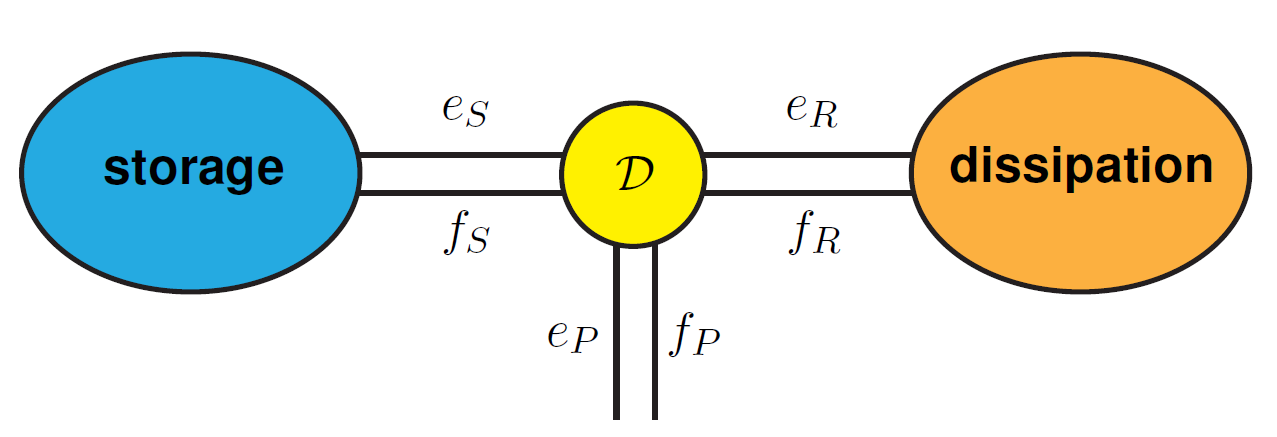
\includegraphics[width=0.55\textwidth]{diracstructure.png}
%	\caption[port-Hamiltonian system structure]{port-Hamiltonian system structure \cite{vanderSchaft_06}}
%	\label{FIG:pHsstructure}
%\end{figure}
\begin{figure}[b!]
	\centering
	\small
	\def\svgwidth{0.6\columnwidth}
	\input{diracstructure.eps_tex}
	\caption{port-Hamiltonian system structure}
	\label{FIG:pHsstructure}
\end{figure}

Complex physical systems can be modelled as a network of energy storing and dissipating elements, \DIFdelbegin \DIFdel{similar }\DIFdelend \DIFaddbegin \DIFadd{for example }\DIFaddend an electrical network consisting of resistors, inductors and capacitors. The rules of interconnection are Newton's third law (action-reaction), Kirchhoff's laws and power-conserving elements like transformers or gyrators. The aim of port-Hamiltonian modelling is to describe the power-conserving elements with the interconnection laws as a geometric structure and to define the Hamiltonian function as the total energy of the system. \\
The \DIFdelbegin \DIFdel{power flowing between }\DIFdelend \DIFaddbegin \DIFadd{input-output pair $(\f{u},\f{y})$ formalizes }\DIFaddend the system's \DIFdelbegin \DIFdel{portions is described by a }\DIFdelend \DIFaddbegin \DIFadd{external energy exchange. The externally supplied energy is internally either stored or dissipated. The flow of stored and dissipated power is also formalized by a power port respectively. All sub-flows and -efforts in the system are elements of a }\DIFaddend general set of flows $\f{f}$ and efforts $\f{e}$\DIFdelbegin \DIFdel{, forming the product $\f{e}^T\f{f}$}\DIFdelend \DIFaddbegin \DIFadd{. The following subsection \ref{SS:PHSinterconnection} gives formal definitions of the internal and external energy exchange of a port-Hamiltonian system}\DIFaddend .

\subsection{Dirac structures and interconnection ports} \label{SS:PHSinterconnection}
The energy-routing structure forms the basis of every port-Hamiltonian system. It can be compared to the printed circuit board in electronics, where capacitors, inductors and resistors are the energy-storing and damping elements. Mathematically it has the form of a \emph{Dirac} structure \cite{vanderSchaft_06}. The main property of a Dirac structure is power conservation, i.e. the power flowing into and out of it always sums to zero. \DIFdelbegin \DIFdel{We can define }\DIFdelend \DIFaddbegin \DIFadd{Thus }\DIFaddend the set of ports $(\f{f},\f{e})$ connecting to the Dirac structure $\mathcal{D}$ \DIFdelbegin \DIFdel{, thus 
}\DIFdelend \DIFaddbegin \DIFadd{has the property 
}\DIFaddend \begin{equation}
\f{e}^T\f{f} = 0 \;  \; \forall (\f{f},\f{e})\in\mathcal{D}
\end{equation}
\DIFdelbegin \DIFdel{Where }\DIFdelend \DIFaddbegin \DIFadd{where }\DIFaddend $\mathcal{D}$ is a subspace of the space of flow and effort $\mathcal{D} \subset \mathcal{E}\times \mathcal{F}$. The space of flows is $\f{f} \in \mathcal{F}$, the space of efforts is its dual linear space $\f{e} \in \mathcal{E} = \mathcal{F}^*$. The Dirac structure has the same dimension \DIFdelbegin \DIFdel{than }\DIFdelend \DIFaddbegin \DIFadd{as }\DIFaddend the space of flows $dim \mathcal{D} = dim \mathcal{F}$.
Further mathematical requirements can be found in literature \cite{vanderSchaft_06,Schaft_14}.\\
Power conservation means that supplied energy is either stored or dissipated in the system. All storing and resistive elements can be \DIFdelbegin \DIFdel{represented each in a single element }\DIFdelend \DIFaddbegin \DIFadd{grouped }\DIFaddend as shown in figure \ref{FIG:pHsstructure}. Three ports join in the interconnection structure, one for \DIFaddbegin \DIFadd{the }\DIFaddend external supply $(\f{u},\f{y})$, one for the sum of storing elements $(\f{f}_\g{S},\f{e}_\g{S})$ and one for the resistive elements $(\f{f}_R,\f{e}_R)$. Mathematically the  interconnection of ports is defined by the Dirac structure matrix \DIFdelbegin \DIFdel{$D$
}\DIFdelend \DIFaddbegin \DIFadd{$S_\mathcal{D}$
}\DIFaddend \begin{equation}\
\begin{pmatrix}
\f{y} \\ \f{f}_\g{S} \\ \f{e}_\g{R}
\end{pmatrix} = \DIFdelbegin \DIFdel{D }\DIFdelend \DIFaddbegin \DIFadd{S_\mathcal{D} }\DIFaddend \begin{pmatrix}
\f{u} \\ \f{e}_\g{S} \\ \f{f}_\g{R}
\end{pmatrix}
\end{equation}
It can be shown that for a skew-symmetric \DIFdelbegin \DIFdel{$D$ }\DIFdelend \DIFaddbegin \DIFadd{$S_\mathcal{D}$ }\DIFaddend the power balance of the ports is
\begin{equation}
{\f{e}_\g{S}}^T\f{f}_\g{S} + {\f{y}}^T\f{u} + {\f{e}_\g{R}}^T\f{f}_\g{R} = 0,
\end{equation}
\DIFdelbegin \DIFdel{This }\DIFdelend \DIFaddbegin \DIFadd{which }\DIFaddend fulfils the desired power conservation.\\
\DIFdelbegin \DIFdel{We can simplify equation \ref{EQ:mechanicalPHS} }\DIFdelend \DIFaddbegin \DIFadd{A further simplification of equation \ref{EQ:mechanicalPHS} is achieved }\DIFaddend by setting $\f{x} = (\f{q}^T,\f{p}^T)^T$\DIFdelbegin \DIFdel{and introduce a general port-Hamiltonian system of the form
}\DIFdelend \DIFaddbegin \DIFadd{. One obtains a generalization to the standard state-space representation
}\DIFaddend \begin{eqnarray}\label{EQ:generalPHS}
\begin{aligned}
\dot{\f{x}} &= [J(\f{x})\DIFdelbegin \DIFdel{-R}\DIFdelend \DIFaddbegin \DIFadd{-D}\DIFaddend (\f{x})]\frac{\partial \mathcal{H}}{\partial \f{x}}(\f{x}) + G(\f{x})\f{u}\\
\f{y} &= G^T(\f{x})\frac{\partial \mathcal{H}}{\partial \f{x}}(\f{x}),
\end{aligned}
\end{eqnarray}
with $J(\f{x}) \in \mathbb{R}^{2k \times 2k}$ being a skew-symmetric structure matrix and \DIFdelbegin \DIFdel{$R(\f{x})  \in  \mathbb{R}^{2k \times 2k}$ }\DIFdelend \DIFaddbegin \DIFadd{$D(\f{x})  \in  \mathbb{R}^{2k \times 2k}$ }\DIFaddend being a positive semi-definite, symmetric dissipation matrix.\DIFaddbegin \\
\DIFadd{Each power port, as shown in \ref{FIG:pHsstructure}, contributes to the energy balance of the system and influences the dynamic behaviour. The external port is used to interconnect two port-Hamiltonian systems.
}\DIFaddend 

\subsubsection{Energy storage port}
The \DIFaddbegin \DIFadd{energy storage }\DIFaddend port accounts for the internal storage of the system, its port variables are $ (\f{f}_\g{S},\f{e}_\g{S}) $. The power supplied through this port is stored in the Hamiltonian energy function $\mathcal{H}(\f{x})$ of the system. The resulting energy balance is:
\begin{equation}\label{EQ:storageport}
	\frac{d}{dt}\mathcal{H} = \frac{\partial^T \mathcal{H}}{\partial \f{x}}(\f{x}) \dot{\f{x}}
\end{equation}
The flow variable is the energy rate $ \f{f}_\g{S} = -\dot{\f{x}} $ and the effort variable is $ \f{e}_\g{S} = \frac{\partial \mathcal{H}}{\partial \f{x}}(\f{x}) $.

\subsubsection{Energy dissipation port}
The \DIFaddbegin \DIFadd{energy dissipation }\DIFaddend port corresponds to internal dissipation and can be used to model resistive elements. The port variables are described by the general resistive relation
\begin{equation}
	F(\f{f}_\g{R},\f{e}_\g{R})=0
\end{equation}
with the property  $ {\f{e}_\g{R}}^T  \f{f}_\g{R} \leq 0 $ (energy dissipation). An important special case is the input-output resistive relation $\f{f}_\g{R} = -F(\f{e}_\g{R})$\DIFdelbegin \DIFdel{, for }\DIFdelend \DIFaddbegin \DIFadd{. For }\DIFaddend linear elements simply
\begin{equation}
\f{f}_\g{R} = -R\f{e}_\g{R} \; , \; R=R^T \succeq 0
\end{equation}
For an uncontrolled system that does not interact with the environment, i.e. \DIFaddbegin \DIFadd{there is }\DIFaddend no energy exchange through the external port, the energy balance is:
\begin{equation}
	\frac{d\mathcal{H}}{dt} = -{\f{e}_\g{S}}^T \f{f}_\g{S} = {\f{e}_\g{R}}^T \f{f}_\g{R} \leq 0
\end{equation}

\subsubsection{External port}
The external port $(\f{u},\f{y})$ can be further split into an environment \emph{interaction} \DIFdelbegin \DIFdel{$(\f{f}^\text{I},\f{e}^\text{I})$ }\DIFdelend \DIFaddbegin \DIFadd{$(\f{f}_\g{I},\f{e}_\g{I})$ }\DIFaddend and a \emph{control} port $(\f{f}_\g{C},\f{e}_\g{C})$, satisfying $\f{y}^T \f{u} = {\f{e}_\g{I}}^T \f{f}_\g{I} + {\f{e}_\g{C}}^T \f{f}_\g{C}$.
The power balance of the whole system then is
\begin{equation}
{\f{e}_\g{S}}^T \f{f}_\g{S} + {\f{e}_\g{R}}^T \f{f}_\g{R} +{\f{e}_\g{I}}^T \f{f}_\g{I} + {\f{e}_\g{C}}^T \f{f}_\g{C} = 0
\end{equation} 
or by using (\ref{EQ:storageport})
\begin{equation}\label{EQ:energybalance}
\frac{d\mathcal{H}}{dt} = {\f{e}_\g{R}}^T \f{f}_\g{R} + {\f{e}_\g{I}}^T\f{f}_\g{I} + {\f{e}_\g{C}}^T \f{f}_\g{C} 
\end{equation}

\subsection{Interconnection of port-Hamiltonian systems}
It is important to notice that the interconnection of two port-Hamiltonian systems is again a port-Hamiltonian system \cite{Schaft_14}. Consider two general systems $(i=1,2)$ with \DIFdelbegin \DIFdel{open }\DIFdelend \DIFaddbegin \DIFadd{yet unconnected }\DIFaddend control and environment interaction ports:
\begin{eqnarray}
\begin{aligned}
	\dot{\f{x}}_i &= \DIFdelbegin \DIFdel{(}\DIFdelend \DIFaddbegin \left[\DIFaddend J_i - R_i\DIFdelbegin \DIFdel{)}\DIFdelend \DIFaddbegin \right] \DIFaddend \frac{\partial \mathcal{H}_i}{\partial \f{x}_i} + \DIFdelbegin \DIFdel{(G_{\g{C},i} }%DIFDELCMD < & %%%
\DIFdel{G_{\g{I},i})}\DIFdelend \DIFaddbegin \begin{pmatrix}G_{\g{C},i} & G_{\g{I},i}\end{pmatrix} \DIFaddend \begin{pmatrix}\f{f}_{\g{C},i} \\ \f{f}_{\g{I},i}\end{pmatrix}\\
	\begin{pmatrix}\f{e}_{\g{C},i} \\ \f{e}_{\g{I},i}\end{pmatrix} &= \begin{pmatrix}G_{\g{C},i}^T \\ G_{\g{I},i}^T\end{pmatrix}\frac{\partial \mathcal{H}_i}{\partial \f{x}_i}
\end{aligned}
\end{eqnarray}
where $J_i,R_i$ are a skew-symmetric structure matrix and a positive semi-definite symmetric dissipation matrix\DIFaddbegin \DIFadd{, respectively}\DIFaddend . The input matrices $G_{\g{C},i},\; G_{\g{I},i}$ describe the effect of a control action and the environment interaction respectively.
For notational convenience the usual dependencies on the states are omitted.\\
The control inputs and outputs are now connected by setting $\f{f}_{\g{C},1} = \f{e}_{\g{C},2} $ and $ \f{f}_{\g{C},2} = -\f{e}_{\g{C},1} $. Note that the minus sign is necessary for power conservation. The power exchanged by the $i$-th system is $P_i = {\f{e}_{\g{C},i}}^T \f{f}_{\g{C},i}$, therefore the total exchanged energy fulfils $ P_1 + P_2 = 0 $. The resulting interconnected system still has the environment interaction ports open:
\begin{eqnarray}
\begin{aligned}
	\dot{\f{x}} &= \DIFdelbegin \DIFdel{(}\DIFdelend \DIFaddbegin \left[\DIFaddend J - R\DIFdelbegin \DIFdel{)}\DIFdelend \DIFaddbegin \right] \DIFaddend \frac{\partial \mathcal{H}}{\partial \f{x}}+ (G_{\g{I},1} & G_{\g{I},2})\DIFdelbegin %DIFDELCMD < \begin{pmatrix}\f{f}_{\g{C},1} \\ \f{f}_{\g{I},2}\end{pmatrix}%%%
\DIFdelend \DIFaddbegin \begin{pmatrix}\f{f}_{\g{I},1} \\ \f{f}_{\g{I},2}\end{pmatrix}\DIFaddend \\
	\begin{pmatrix}\f{e}_{\g{I},1} \\ \f{e}_{\g{I},2}\end{pmatrix} &= \begin{pmatrix}G_{\g{I},1}^T \\ G_{\g{I},2}^T\end{pmatrix}\frac{\partial \mathcal{H}}{\partial \f{x}}
\end{aligned}
\end{eqnarray}
where $ \f{x} = (\f{x}_1^T, \f{x}_2^T)^T $ and $\mathcal{H}  = \mathcal{H}_1 + \mathcal{H}_2 $ is the sum of the two energies. The structure and dissipation matrix become:
\[J = \begin{pmatrix} J_1 & G_{\g{C},1} G_{\g{C},2}^T \\ 
-G_{\g{C},2} G_{\g{C},1}^T & J_2\end{pmatrix} \, , \; 
\DIFdelbegin \DIFdel{R }\DIFdelend \DIFaddbegin \DIFadd{D }\DIFaddend = \DIFdelbegin %DIFDELCMD < \begin{pmatrix}
%DIFDELCMD < R_1 & 0 \\ 0 & R_2\end{pmatrix}%%%
\DIFdelend \DIFaddbegin \begin{pmatrix}
D_1 & 0 \\ 0 & D_2\end{pmatrix}\DIFaddend \]

\subsection{port-Hamiltonian systems and passivity}\DIFaddbegin \label{SS:Passivity}
\DIFaddend A system is \emph{passive} \DIFaddbegin \DIFadd{\mbox{%DIFAUXCMD
\cite{Ortega_01}}%DIFAUXCMD
, }\DIFaddend if there exists a differentiable storage function $\mathcal{H}(\f{x}) \geq 0$ that satisfies 
\begin{equation}\label{EQ:PassivityDefinition}
\frac{d}{dt}\mathcal{H}(\f{x}(t)) \leq \f{u}^T(t) \f{y}(t)
\end{equation}
The product of the input-output pair $(\f{u},\f{y})$ is the supplied power. By definition the Hamiltonian function represents the total energy stored in the system. For a port-Hamiltonian system of the form of equation (\ref{EQ:generalPHS}) \DIFdelbegin \DIFdel{we have
}\DIFdelend \DIFaddbegin \DIFadd{the energy balance is
}\DIFaddend \begin{eqnarray}
\begin{aligned}
\frac{d}{dt}\mathcal{H}(\f{x}) &= \frac{\partial^T \mathcal{H}}{\partial \f{x}} \frac{d\f{x}}{dt} = \frac{\partial^T \mathcal{H}}{\partial \f{x}}\left[(J(\f{x})\DIFdelbegin \DIFdel{-R}\DIFdelend \DIFaddbegin \DIFadd{-D}\DIFaddend (\f{x}))\frac{\partial \mathcal{H}}{\partial \f{x}} + G(\f{x})\f{u}\right]  \\
&= \frac{\partial^T \mathcal{H}}{\partial \f{x}}J(\f{x})\frac{\partial \mathcal{H}}{\partial \f{x}} - \frac{\partial^T \mathcal{H}}{\partial \f{x}}\DIFdelbegin \DIFdel{R}\DIFdelend \DIFaddbegin \DIFadd{D}\DIFaddend (\f{x})\frac{\partial \mathcal{H}}{\partial \f{x}} + (G^{-T}(\f{x})e)^T G(\f{x})\f{u}  \\
&= \f{y}^T\f{u} - \frac{\partial^T \mathcal{H}}{\partial \f{x}}\DIFdelbegin \DIFdel{R}\DIFdelend \DIFaddbegin \DIFadd{D}\DIFaddend (\f{x})\frac{\partial \mathcal{H}}{\partial \f{x}}
\end{aligned}
\end{eqnarray}
The property $\frac{\partial^T \mathcal{H}}{\partial \f{x}}J(\f{x})\frac{\partial \mathcal{H}}{\partial \f{x}}=0$ holds for a skew symmetric matrix $J(\f{x}) = -J(\f{x})^T$. The product of the \DIFdelbegin \DIFdel{effort-flow pair $\f{e}^T\f{f}$ }\DIFdelend \DIFaddbegin \DIFadd{input-output pair $\f{y}^T\f{u}$ }\DIFaddend is the power supplied to the system. Since \DIFdelbegin \DIFdel{$R(\f{x})=R(\f{x})^T \succeq 0$ }\DIFdelend \DIFaddbegin \DIFadd{$D(\f{x})=D(\f{x})^T \succeq 0$ }\DIFaddend is symmetric and positive semi-definite, \DIFdelbegin \DIFdel{we have $\frac{\partial^T \mathcal{H}}{\partial \f{x}}R(\f{x})\frac{\partial \mathcal{H}}{\partial \f{x}} \geq 0$. Conclusively equation (\ref{EQ:PassivityDefinition}) holds for }\DIFdelend \DIFaddbegin \DIFadd{it is $\frac{\partial^T \mathcal{H}}{\partial \f{x}}D(\f{x})\frac{\partial \mathcal{H}}{\partial \f{x}} \geq 0$. Conclusively }\DIFaddend every port-Hamiltonian system\DIFaddbegin \DIFadd{, }\DIFaddend that satisfies the properties \DIFdelbegin \DIFdel{of }\DIFdelend equation (\ref{EQ:generalPHS}), \DIFdelbegin \DIFdel{clearly the system is }\emph{\DIFdel{passive}}%DIFAUXCMD
\DIFdelend \DIFaddbegin \DIFadd{is passive in the sense of equation \ref{EQ:PassivityDefinition}}\DIFaddend . If $R=0$, i.e. the system exhibits no dissipation \DIFdelbegin \DIFdel{we call it }\DIFdelend \DIFaddbegin \DIFadd{and is termed as }\DIFaddend \emph{lossless}.
\DIFdelbegin %DIFDELCMD < \\
%DIFDELCMD < %%%
\DIFdelend Passivity is a sufficient criterion for asymptotic stability \cite{Ortega_01}.  
\DIFaddbegin 


\DIFaddend \section{3D-space modelling of mechanical systems}\label{S:3Dspace-modelling}


\subsection{Euclidean space and motions}\label{[SS:euclideanspacemotions]}
\subsubsection{Coordinate frames}
A coordinate frame of the three-dimensional Euclidean space is a 4-tuple of the form $ \Psi = (\f{o},\hat{\f{x}},\hat{\f{y}},\hat{\f{z}})$\DIFdelbegin \DIFdel{. Where }\DIFdelend \DIFaddbegin \DIFadd{, where }\DIFaddend $ \f{o} $ is the three-dimensional vector of the origin and $ \hat{\f{x}},\hat{\f{y}},\hat{\f{z}} $ are the linear independent, orthonormal coordinate vectors. Consider two coordinate frames $ {\Psi}_1,{\Psi}_2 $ which share the same origin but differ in orientation due to different choices of $ \hat{\f{x}}_i,\hat{\f{y}}_i,\hat{\f{z}}_i, \; i=1,2 $. The change of orientation from $ {\Psi}_i $ to $ {\Psi}_j $ is described by the rotation matrix $ \g{R}_i^j $. The set of rotation matrices is called \emph{special orthonormal} group ($SO(3)$) \cite{Stramigioli_01b} and is defined as:
\begin{equation}
	SO(3) = \{\g{R} \in \mathbb{R}^{3 \times 3} \; | \; \g{R}^{-1} = \g{R}^T, \DIFdelbegin \DIFdel{det }\DIFdelend \DIFaddbegin \DIFadd{\text{det} }\DIFaddend \g{R} = 1\}
\end{equation}
\DIFdelbegin \DIFdel{Usually coordinate frames are defined with respect to an inertial frame, and the coordinate vectors $ \hat{\f{x}},\hat{\f{y}},\hat{\f{z}} $ are chosen equal for all frames, deviations of orientation are represented by a rotation matrix relative to the }\DIFdelend \DIFaddbegin \DIFadd{Sometimes it is useful to define non-inertial frames, e.g. attached to a rigid body. Generally these frames do not share the origin with a the }\DIFaddend inertial frame. \DIFdelbegin \DIFdel{In general a change of coordinate frames from $ \Psi_i $ to $ \Psi_j $ can be expressed with the homogeneous matrix
}\[ \DIFdel{H_i^j := \begin{pmatrix}\g{R}_i^j & \f{p}_i^j \\ 0_{1\times3} & 1\end{pmatrix} }\]
%DIFAUXCMD
\DIFdel{where }\DIFdelend \DIFaddbegin \DIFadd{Consider two frames $ {\Psi}_i,{\Psi}_j $ with different origins then  }\DIFaddend $\f{p}_i^j = \f{o}_j - \f{o}_i$ denotes the distance between the origins. \DIFaddbegin \DIFadd{In general, a change between coordinate frames, which differ in position and orientation is expressed with the homogenous matrix
}\begin{equation} \DIFadd{H_i^j := \begin{pmatrix}\g{R}_i^j & \f{p}_i^j \\ \f{0}_{1\times3} & 1\end{pmatrix} }\end{equation}
\DIFaddend A point $ \f{p}^i \in \mathbb{R}^3 $ expressed in $ {\Psi}_i $ is cast into ${\Psi}_j$ by
\begin{equation}\label{EQ:coordchange}
	\begin{pmatrix}\f{p}^j \\ 1\end{pmatrix} = H_i^j \begin{pmatrix}
		\f{p}^i \\ 1\end{pmatrix}
\end{equation}.
The inverse transformation $ H_j^i $ is given by 
\DIFdelbegin \[\DIFdel{H_i^j = (H_i^j)^{-1} = \begin{pmatrix}(\g{R}_i^j)^T & -(\g{R}_i^j)^T \f{p}_i^j \\ 0_{1 \times 3} & 1\end{pmatrix} }\]
%DIFAUXCMD
\DIFdelend \DIFaddbegin \begin{equation}\DIFadd{H_i^j = (H_i^j)^{-1} = \begin{pmatrix}(\g{R}_i^j)^T & -(\g{R}_i^j)^T \f{p}_i^j \\ \f{0}_{1 \times 3} & 1\end{pmatrix} }\end{equation}
\DIFaddend and is still a homogeneous matrix.
The set of homogeneous matrices is called the \emph{special Euclidean} group:
\begin{equation}
	SE(3) := \{\DIFdelbegin %DIFDELCMD < \begin{pmatrix}\g{R} & \f{p}\\0 & 1\end{pmatrix} %%%
\DIFdelend \DIFaddbegin \begin{pmatrix}\g{R} & \f{p}\\\f{0} & 1\end{pmatrix} \DIFaddend \; | \; \g{R} \in SO(3), \f{p} \in \mathbb{R}^3\} 
\end{equation}
The $SE(3)$ is a matrix Lie group, composed of the set of homogeneous matrices $H_i^j$ and the matrix multiplication being the group operation. For more information on Lie groups see e.g. \cite{Stramigioli_01}.
\subsubsection{Twists and wrenches}
Consider any point \DIFdelbegin \DIFdel{$ \f{p} $ }\DIFdelend \DIFaddbegin \DIFadd{$ \f{p}^i $ }\DIFaddend not moving in \DIFdelbegin \DIFdel{coordinate frames }\DIFdelend \DIFaddbegin \DIFadd{the coordinate frame }\DIFaddend $\Psi_i $, i.e. $ \dot{\f{p}}^i = 0 $. If $ \f{p} $ is moving in another coordinate frame $ \Psi_j $, the two \DIFdelbegin \DIFdel{frame }\DIFdelend \DIFaddbegin \DIFadd{frames }\DIFaddend move with respect to each other. The trajectory can be described as a function of time: $H_i^j(t) \in SE(3)$. By differentiating (\ref{EQ:coordchange}) one obtains
\[\DIFdelbegin %DIFDELCMD < \begin{pmatrix}\dot{\f{p}}^j(t) \\ 1\end{pmatrix} %%%
\DIFdelend \DIFaddbegin \begin{pmatrix}\dot{\f{p}}^j(t) \\ 0\end{pmatrix} \DIFaddend = \dot{H}_i^j(t) \begin{pmatrix}\f{p}^i \\ 1\end{pmatrix} \]
$ \dot{H}_i^j $ describes both motion and a change of the reference frame. A \DIFdelbegin \DIFdel{separated representationis
}\DIFdelend \DIFaddbegin \DIFadd{representation, that separates  $\dot{H}_i^j$ into a homogeneous matrix $H_i^j$ and a velocity variable (twist) $\tilde{T}_i^{j,j}$, is 
}\DIFaddend \begin{equation}\label{EQ:twistrighttranslation}
	\DIFdelbegin %DIFDELCMD < \begin{pmatrix}\dot{\f{p}}^j(t) \\ 1\end{pmatrix} %%%
\DIFdelend \DIFaddbegin \begin{pmatrix}\dot{\f{p}}^j(t) \\ 0\end{pmatrix} \DIFaddend = \tilde{T}_i^{j,j}\left(H_i^{j}\begin{pmatrix}\f{p}^i \\ 1\end{pmatrix}\right)
\end{equation}
$ \dot{H}_i^j$ is a tangential vector along the trajectory $H_i^j(t)$ and thus in the tangent space of the $SE(3)$: $ \dot{H}_i^j \in T_{H_i^j}SE(3)$. To obtain a representation of motion which is referenced to a coordinate frame, \DIFdelbegin \DIFdel{we }\DIFdelend \DIFaddbegin \DIFadd{one }\DIFaddend can map $\dot{H}_i^j$ to the identity of the $SE(3)$. At the identity $ e $ of the $SE(3)$ the tangent space $ T_e SE(3) $ has the structure of a Lie algebra. The Lie algebra of the $SE(3)$ is denoted by $\mathfrak{se}(3)$. This is done either by left or right translation, for a definition see \cite{Stramigioli_01}. The right translation is used in (\ref{EQ:twistrighttranslation}) and is written compactly
\begin{equation}\label{EQ:righttranslation}
\dot{H}_i^j = \tilde{T}_i^{j,j} H_i^j
\end{equation}\label{EQ:lefttranslation}
The left translation leads to
\begin{equation}
\dot{H}_i^j = H_i^j \tilde{T}_i^{i,j} 
\end{equation}
\DIFaddbegin 

\DIFadd{Left and right translations lead to different representations of a twist:
}\begin{itemize}
	\item \DIFadd{$T_i^{k,j}$ is the twist of $\Psi_i$ with respect to $\Psi_j$ expressed in the frame $\Psi_k$
	}\item \DIFadd{$T_i^j = T_i^{j,j}$ is the twist of $\Psi_i$ with respect to $\Psi_j$ expressed naturally in $\Psi_j$ 
}\end{itemize}

\DIFaddend We call $\tilde{T} \in T_e SE(3)$ a twist and the $\mathfrak{se}(3)$ the space of twists.
\DIFdelbegin \DIFdel{Let us look more closely at this representation by calculating the twist }\DIFdelend \DIFaddbegin 

\DIFadd{To understand the formalism of a twist to describe motion, the derivation }\DIFaddend from the elements of \DIFdelbegin \DIFdel{the homogeneous matrix }\DIFdelend \DIFaddbegin \DIFadd{a homogeneous matrix allows to identify its components
}\DIFaddend 

\begin{eqnarray}\label{EQ:twistdecomposition}
\begin{aligned}
\DIFdelbegin \DIFdel{T}\DIFdelend \DIFaddbegin \tilde{T}\DIFaddend _i^j &= \dot{H}_i^j H_j^i =
\DIFdelbegin %DIFDELCMD < \begin{pmatrix}
%DIFDELCMD < \dot{\g{R}}_i^j & \dot{\f{p}}_i^j \\ 0 & 0
%DIFDELCMD < \end{pmatrix}
%DIFDELCMD < \begin{pmatrix}
%DIFDELCMD < \g{R}_j^i & \f{p}_j^i \\ 0 & 1
%DIFDELCMD < \end{pmatrix} %%%
\DIFdelend \DIFaddbegin \begin{pmatrix}
\dot{\g{R}}_i^j & \dot{\f{p}}_i^j \\ \mathbf{0} & 0
\end{pmatrix}
\begin{pmatrix}
\g{R}_j^i & \f{p}_j^i \\ \mathbf{0} & 1
\end{pmatrix} \DIFaddend = 
\DIFdelbegin %DIFDELCMD < \begin{pmatrix}
%DIFDELCMD < \dot{\g{R}}_i^j & \dot{\f{p}}_i^j \\ 0 & 0
%DIFDELCMD < \end{pmatrix}
%DIFDELCMD < \begin{pmatrix}
%DIFDELCMD < (\g{R}_i^j)^T & -(\g{R}_i^j)^T \f{p}_i^j \\ 0 & 1
%DIFDELCMD < \end{pmatrix} %%%
\DIFdelend \DIFaddbegin \begin{pmatrix}
\dot{\g{R}}_i^j & \dot{\f{p}}_i^j \\ \mathbf{0} & 0
\end{pmatrix}
\begin{pmatrix}
{\g{R}_i^j}^T & -{\g{R}_i^j}^T \f{p}_i^j \\ \mathbf{0} & 1
\end{pmatrix} \DIFaddend \\ 
&= 
\DIFdelbegin %DIFDELCMD < \begin{pmatrix}
%DIFDELCMD < \dot{\g{R}}_i^j(\g{R}_i^j)^T & -\dot{\g{R}}_i^j(\g{R}_i^j)^T\ \f{p}_i^j + \dot{\f{p}}_i^j \\ 0 & 0
%DIFDELCMD < \end{pmatrix} %%%
\DIFdelend \DIFaddbegin \begin{pmatrix}
\dot{\g{R}}_i^j{\g{R}_i^j}^T & -\dot{\g{R}}_i^j{\g{R}_i^j}^T\ \f{p}_i^j + \dot{\f{p}}_i^j \\ \mathbf{0} & 0
\end{pmatrix} \DIFaddend =: 
\DIFdelbegin %DIFDELCMD < \begin{pmatrix}
%DIFDELCMD < \tilde{\omega}_i^j & \f{v}_i^j \\ 0 & 0
%DIFDELCMD < \end{pmatrix}
%DIFDELCMD < %%%
\DIFdelend \DIFaddbegin \begin{pmatrix}
\tilde{\omega}_i^j & \f{v}_i^j \\ \mathbf{0} & 0
\end{pmatrix}
\DIFaddend \end{aligned}
\end{eqnarray}
It is clear from this equation that the linear velocity part $\f{v}_i^j$ is not the velocity of the frame $\Psi_i$ with respect to $\Psi_j$, identified by $\dot{\f{p}}_i^j$. This twist representation is described by the \emph{screw theory} (see e.g. \cite{KinematicsHandbook}). It can be visualized by the angular velocity around an axis and the linear velocity along this axis.



Next to the $4  \times 4$ matrix $\tilde{T} $ there exists also a vector representation $T\in \mathbb{R}^6$
\begin{equation}
 \tilde{T} = \DIFdelbegin %DIFDELCMD < \begin{pmatrix}\tilde{\omega} & \f{v} \\ 0 & 0\end{pmatrix} %%%
\DIFdelend \DIFaddbegin \begin{pmatrix}\tilde{\omega} & \f{v} \\ \mathbf{0} & 0\end{pmatrix} \DIFaddend \; , \; T = \begin{pmatrix} \boldsymbol{\omega} \\ \f{v}\end{pmatrix} \end{equation}
wherein $\f{v} \in \mathbb{R}^3$ is the linear velocity and $\boldsymbol{\omega} \in \mathbb{R}^3$ is the angular velocity. $\tilde{\omega} \in \mathbb{R}^{3 \times 3}$ is the skew-symmetric representation of the vector $\boldsymbol{\omega}$
\begin{equation}\label{EQ:skewsymmetricop}
\boldsymbol{\omega} = \begin{pmatrix}
\omega_1 \\ \omega_2 \\ \omega_3\end{pmatrix} \; \Rightarrow \; \tilde{\omega} = \begin{pmatrix}0 & -\omega_3 & \omega_2 \\ \omega_3 & 0 & \omega_1 \\ -\omega_2 & \omega_1 & 0\end{pmatrix} \end{equation} \\
\DIFaddbegin \DIFadd{Throughout this thesis, vectors assigned with a tilde operator $\tilde{\bullet}$ denote the matrix representation of the vector. This is the matrix crossproduct for a vector of dimension $\mathbb{R}^3$, or the $4\times 4$ representation for a $\mathbb{R}^6$ vector.
}\DIFaddend 

\DIFdelbegin \DIFdel{Left and right translations lead to different representations of a twist:
}%DIFDELCMD < \begin{itemize}
%DIFDELCMD < \item %%%
\DIFdel{$T_i^{k,j}$ is the twist of $\Psi_i$ with respect to $\Psi_j$ expressed in the frame $\Psi_k$
}%DIFDELCMD < \item %%%
\DIFdel{$T_i^j = T_i^{j,j}$ is the twist of $\Psi_i$ with respect to $\Psi_j$ expressed naturally in $\Psi_j$ 
}%DIFDELCMD < \end{itemize}
%DIFDELCMD < 

%DIFDELCMD < %%%
\DIFdelend Changes of coordinates for twists are of the form 
\begin{equation}
\tilde{T}_i^{j,j} = \tilde{T}_i^{j} = H_i^j \tilde{T}_i^{i,j} H_j^i\end{equation}
or for the vector representation
\begin{equation}
 T_i^{j} = Ad_{H_i^j} T_i^{i,j} \; , \;
Ad_{H_i^j} = \begin{pmatrix}R_i^j & 0 \\ \tilde{p}_i^j R_i^j & R_i^j\end{pmatrix} \end{equation}

The  dual vector space of $\mathfrak{se}(3)$ is the space of linear operations from $\mathfrak{se}(3)$ to $\mathbb{R} $. It is denoted by $\mathfrak{se}^*(3)$ and represents the space of wrenches $W$. Wrenches decompose to moments \DIFdelbegin \DIFdel{$ \f{m} \in \mathbb{R}^3 $ and forces $ \textbf{f} \in \mathbb{R}^3 \in \mathbb{R}^3$.
}\DIFdelend \DIFaddbegin \DIFadd{$ \mathbf{{m}} \in \mathbb{R}^3 $ and forces $ \textbf{f} \in \mathbb{R}^3$.
}\DIFaddend \begin{equation}
 W = ( \DIFdelbegin %DIFDELCMD < \f{m} %%%
\DIFdelend \DIFaddbegin \DIFadd{\mathbf{m} }\DIFaddend \;\; \textbf{f}) \; , \; \tilde{W} = \DIFdelbegin %DIFDELCMD < \begin{pmatrix}
%DIFDELCMD < \tilde{m} & \textbf{f} \\ 0 & 0\end{pmatrix} %%%
\DIFdelend \DIFaddbegin \begin{pmatrix}
\tilde{\g{m}} & \textbf{f} \\ \mathbf{0} & 0\end{pmatrix} \DIFaddend \end{equation}
Again $\tilde{W} \in \mathbb{R}^{4\times 4}$ is a matrix while $W \in \mathbb{R}^6$ is the  row vector representation.
The change of coordinates for \DIFdelbegin \DIFdel{twists }\DIFdelend \DIFaddbegin \DIFadd{wrenches }\DIFaddend is similar to the case of twists:
\begin{equation}
(W_i^{k,i})^T = Ad_{H_k^i}^T (W_i\DIFdelbegin \DIFdel{^i}\DIFdelend \DIFaddbegin \DIFadd{^{i,i}}\DIFaddend )^T \end{equation} 
Here the mapping is in the opposite direction, from $\Psi_j$ to $\Psi_i$, \DIFdelbegin \DIFdel{what }\DIFdelend \DIFaddbegin \DIFadd{which }\DIFaddend is a consequence of the fact that wrenches are duals to twists. Again there are different representations of wrenches: \begin{itemize}
\item $W_i^{k,j}$ is the wrench applied to a spring connecting $\Psi_i$ to $\Psi_j$ on the side of $\Psi_i$ expressed in the coordinate frame $\Psi_k$.
\item $W_i^k $ is the wrench applied to a body attached to $\Psi_i$ expressed in the coordinate frame $\Psi_k$.
\end{itemize}
These definitions lead to the following rules of interconnection:
\DIFdelbegin \DIFdel{Connecting a body }\DIFdelend \DIFaddbegin \DIFadd{connecting a mass }\DIFaddend and spring in the point $\Psi_i$ and applying the principle of action and reaction \DIFdelbegin \DIFdel{we get }\DIFdelend \DIFaddbegin \DIFadd{one gets }\DIFaddend $W_i^{k,j} = -W_i^k$. \DIFdelbegin \DIFdel{Due to the nodicity }\DIFdelend \DIFaddbegin \DIFadd{The wrenches on either side }\DIFaddend of a spring \DIFdelbegin \DIFdel{we have }\DIFdelend \DIFaddbegin \DIFadd{are antisymmetric  }\DIFaddend $ W_i^{k,j} = -W_j^{k,i} $\\
\DIFdelbegin %DIFDELCMD < 

%DIFDELCMD < %%%
\DIFdel{We define power flowing through a port by the }\DIFdelend \DIFaddbegin \DIFadd{The }\DIFaddend duality product of flow and effort \DIFaddbegin \DIFadd{defines the power flowing through a port}\DIFaddend , in the mechanical domain this \DIFdelbegin \DIFdel{twist and }\DIFdelend \DIFaddbegin \DIFadd{corresponds to the twist and the }\DIFaddend wrench. On a vector space level the power port $\mathcal{P}$ is defined by the Cartesian product of the Lie algebra $\mathfrak{se}(3)$ and its dual $\mathfrak{se}^*(3)$: $\mathcal{P} = \mathfrak{se}(3) \times \mathfrak{se}^*(3)$.

\subsection{Input-state-output port-Hamiltonian systems in 3D space}
The \DIFdelbegin \DIFdel{simple relation , between }\DIFdelend \DIFaddbegin \DIFadd{port-Hamiltonian systems considered so far define the relation of }\DIFaddend the time-derivative of the configuration \DIFaddbegin \DIFadd{$\f{q}$ }\DIFaddend and the change of kinetic energy
\DIFdelbegin \DIFdel{, $\frac{\partial \mathcal{H}}{\partial \f{p}}=\dot{\f{q}}$ does not hold for a 3D-mechanical system. It is detailed in the next subsection that $\frac{\partial \mathcal{H}}{\partial P_i^i} = T_i^{i,0} = H_0^i \dot{H_i^0}$, with the $H_0^i$ being the configuration variable and $P_i^i$ the momentum }\DIFdelend \DIFaddbegin \begin{equation}
	\DIFadd{\frac{\partial \mathcal{H}}{\partial \f{p}}= M^{-1} \f{p} = \dot{\f{q}}
}\end{equation}
\DIFadd{For six DoF configuration and twist are related by $\dot{H}_i^j = \tilde{T}_i^{j,j} H_i^j$ (eq. \ref{EQ:lefttranslation}). The next section introduces the 3D-description of a mass in the port-Hamiltonian framework, the kinetic (co-)energy function is $\mathcal{H}_{\g{K}} = \frac{1}{2} {P_i^i}^T M^{-1} P_i^i$, with the momentum $P_i^i = M T_i^{i,0}$}\DIFaddend . Thus the \DIFaddbegin \DIFadd{relation of configuration- and kinetic energy change for six DoF is 
}\begin{equation}
 \DIFadd{\frac{\partial \mathcal{H}}{\partial P_i^i} = M^{-1} P_i^i = H_0^i \dot{H_i^0}
}\end{equation}
 \DIFadd{Consequently the }\DIFaddend interconnecting Dirac structure depends on the configuration $H_0^i$ and \DIFdelbegin \DIFdel{we call it }\DIFdelend \DIFaddbegin \DIFadd{is termed }\DIFaddend a \emph{modulated} Dirac structure. Mathematically the state space of the system is then a \emph{manifold}, for details see \cite{Schaft_14}. \DIFdelbegin \DIFdel{We define local coordinates $\f{x}$ on the }\DIFdelend \DIFaddbegin \DIFadd{This }\DIFaddend state manifold $\mathcal{X}$ \DIFdelbegin \DIFdel{, associate the }\DIFdelend \DIFaddbegin \DIFadd{includes the local coordinates $\f{x} \in \mathcal{X}$. The }\DIFaddend flows towards the energy storage \DIFaddbegin \DIFadd{is assigned }\DIFaddend with $\f{f}_\g{S} = -\dot{\f{x}}$ and the efforts with \DIFdelbegin \DIFdel{$\f{e}_\g{S} = \frac{\partial V}{\partial \f{x}}$}\DIFdelend \DIFaddbegin \DIFadd{$\f{e}_\g{S} = \frac{\partial \mathcal{H}}{\partial \f{x}}$}\DIFaddend . The flows are elements of the tangent space $T_x\mathcal{X}$ of the state manifold at the state $\f{x} \in \mathcal{X}$ and the efforts are elements of the co-tangent space $T_x^*\mathcal{X}$. The resulting port-Hamiltonian system in 3D space is of the form
\begin{eqnarray}
\begin{aligned}
\dot{\f{x}} &= [J(\f{x})\DIFdelbegin \DIFdel{-R}\DIFdelend \DIFaddbegin \DIFadd{-D}\DIFaddend (\f{x})]\frac{\partial \mathcal{H}}{\partial \f{x}}(\f{x}) + G(\f{x}) \f{u} \\
\f{y} &= G^T(\f{x})\frac{\partial \mathcal{H}}{\partial \f{x}}\DIFaddbegin \DIFadd{(x)
}\DIFaddend \end{aligned}
\end{eqnarray}
with a skew-symmetric matrix $J(\f{x})$ and a resistive structure matrix \DIFdelbegin \DIFdel{$R(\f{x})$ }\DIFdelend \DIFaddbegin \DIFadd{$D(\f{x})$ }\DIFaddend which is symmetric and positive semi-definite. Clearly $\f{u}$ and $\f{y}$ denote the input and output respectively and this representation is again of the \emph{input-state-output} form. In the following section \DIFdelbegin \DIFdel{we introduce }\DIFdelend \DIFaddbegin \DIFadd{introduces }\DIFaddend the corresponding representations of atomic mechanical elements.




\subsection{\DIFdelbegin \DIFdel{Dynamics }\DIFdelend \DIFaddbegin \DIFadd{Modelling }\DIFaddend of \DIFdelbegin \DIFdel{physical components}\DIFdelend \DIFaddbegin \DIFadd{atomic mechanical elements}\DIFaddend }\label{SS:DynamicsPhysicalComponents}
\subsubsection{Springs}
A \emph{spring} is the ideal, lossless element storing potential energy. It is connected to two bodies and is defined by a potential energy function. The energy is a function of the relative displacement of the attached bodies. Consider a spring between the two bodies $ B_i $ and $ B_j $,  with coordinate frames $ \Psi_i $ and $ \Psi_j $ fixed to the respective \DIFdelbegin \DIFdel{body}\DIFdelend \DIFaddbegin \DIFadd{bodies}\DIFaddend . The stored potential energy is positive definite function of the form 
\begin{equation}\label{EQ:SpringEnergyFunction}
	V_{\g{P}} : SE(3) \rightarrow \mathbb{R}; \; H_i^j \mapsto V_{\g{P}}(H_i^j)
\end{equation}
For explicit energy functions for different types of springs see \cite{Stramigioli_01}.
The input-state-output form is defined by the relative displacement $H_i^j$ (state variable), the wrench $W_i^{j,j}$ (\DIFdelbegin \DIFdel{effort}\DIFdelend \DIFaddbegin \DIFadd{output}\DIFaddend ) and the twist $T_i^j$ (\DIFdelbegin \DIFdel{flow}\DIFdelend \DIFaddbegin \DIFadd{input}\DIFaddend ).
\begin{eqnarray}
\begin{aligned}
	&\dot{H}_i^j = T_i^{j}H_i^j\\
	&W_i^{j,j} = \frac{\partial V_{\g{P}}(H_i^j)}{\partial H_i^j}(H_i^j)^T
\end{aligned}
\end{eqnarray}
Note that $ V_{\g{P}} $ is an energetic minimum when $ H_i^j $ is the identity matrix $I_4$. An energetic minimum is physically necessary, otherwise infinite energy would be extractable from the spring. With $ H_i^j = I_4 $ the frames $ \Psi_i $ and $\Psi_j$ coincide.
It is possible to define springs with non-zero rest-length by introducing coordinate frames $ \Psi_{ic} $ and $\Psi_{jc}$ rigidly attached to $ \Psi_i $ and $\Psi_j$ respectively. The spring is now between the new frames, thus the energetic minimum is $H_{ic}^{jc} = I_4$. The displacements $ H_i^{ic}, H_j^{jc} $ are the resulting rest-lengths. Frames $ \Psi_{ic} $ and $\Psi_{jc}$ can be chosen to represent the \emph{center of stiffness}, where translation and rotation are maximally decoupled \cite{Stramigioli_99}.

\DIFaddbegin \begin{figure}[h!]
	\centering
	\small
	\def\svgwidth{0.8\columnwidth}
	\input{variablespring.eps_tex}
	\caption{\DIFaddFL{Frames and configurations for a variable-restlength spring}}
	\label{FIG:variablespring}
\end{figure}



\DIFaddend \begin{comment}
\subsubsection{Variable rest-length springs}
Varying the rest-lengths of springs in manipulator-object interaction allows to perform a grasp and specify grasping forces. The rest-length influences the energy configuration, to allow for controlled changes of rest-length an additional power port is introduced. The chosen hinge points $ \Psi_b,\Psi_j $ of the spring define an axis, known as the principal axes of stiffness. Changes of the rest-length leave this axis unaffected, i.e. the displacement is in-line. With reference to Fig. \ref{FIG:variablespring}, the change of rest-length is a change of relative displacement of $ \Psi_b $ and $\Psi_i$: $H_i^b$.
\begin{figure}[htb]
	\centering
	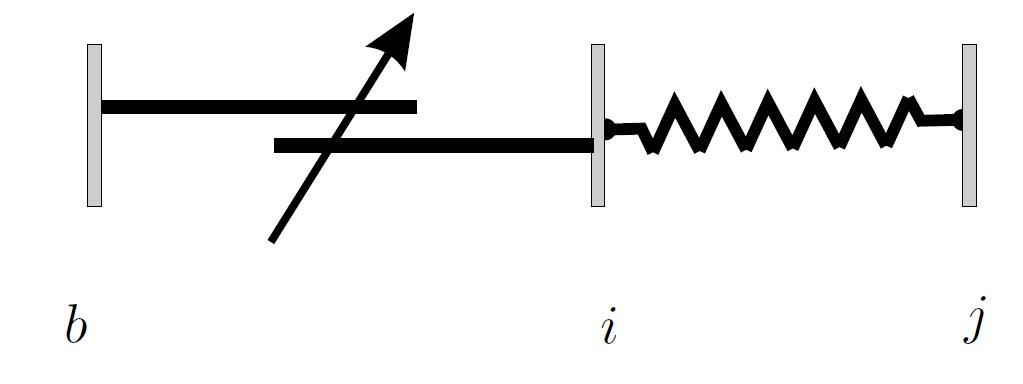
\includegraphics[width=0.55\textwidth]{variablespring.jpg}
	\caption[Variable rest-length spring]{Variable rest-length spring \cite{Stramigioli_99}}
	\label{FIG:variablespring}
\end{figure}
Towards a port-Hamiltonian representation we need to identify the components contributing to the deformation twist of the spring $ T_i^{j} $: the displacement twist of the bodies attached to the spring $T_b^{j} $ and the twist resulting from a commanded change of the rest-length $T_i^{b}$ \cite{Stramigioli_01c}.
\begin{equation}
	T_i^{j} = T_b^{j} + Ad_{H_b^j} T_i^{b}
\end{equation}
Since no additional energy storages were introduced, the Hamiltonian function is equal to the case of the simple spring. We can write the two-port Hamiltonian system of a variable length spring as
\begin{eqnarray}\label{EQ:variablerestlengthspring}
\begin{aligned}
	&\dot{H}_i^j =\left( \begin{pmatrix}1 & Ad_{H_b^j}\end{pmatrix} \begin{pmatrix}T_b^{j} \\ T_i^{b}\end{pmatrix} \right) H_i^j\\
	&\begin{pmatrix}W_b^{j,j} \\ W_i^{b,b}\end{pmatrix}  = \left( \begin{pmatrix}1 \\ Ad_{H_b^j}^T\end{pmatrix} \frac{\partial V_{i,j}}{\partial H_i^j} \right) (H_i^j)^T
\end{aligned}
\end{eqnarray}
\end{comment}

\subsubsection{Inertias}
Inertias are special since they in general store two types of energy: kinetic and potential energy due to gravitation. \DIFdelbegin \DIFdel{At first we exclude }\DIFdelend \DIFaddbegin \DIFadd{For simplicity }\DIFaddend the gravitational terms \DIFdelbegin \DIFdel{and }\DIFdelend \DIFaddbegin \DIFadd{are excluded at first to allow }\DIFaddend focus on motion. Kinetic energy is a function of the relative motion w.r.t. an inertial reference. When expressing motion in non-inertial or accelerated reference frames, fictitious forces such as the \emph{Coriolis} or the \emph{centrifugal} force need to be considered.\\
\DIFdelbegin \DIFdel{Let us start }\DIFdelend \DIFaddbegin \DIFadd{The derivation of the port-Hamiltonian formulation starts }\DIFaddend from \emph{Newton's} second law of dynamics\DIFdelbegin \DIFdel{, the }\DIFdelend \DIFaddbegin \DIFadd{. The }\DIFaddend time derivative of a body's momentum is equal to the applied wrench.
\begin{equation}
\dot{P}_b^0 = W_b^0
\end{equation}
The momentum of the inertia $b$ and the wrench acting on it are both expressed in the inertial reference frame $\Psi_0$. \DIFdelbegin \DIFdel{Let us consider }\DIFdelend \DIFaddbegin \DIFadd{Consider }\DIFaddend the non-inertial frame $\Psi_b$, \DIFdelbegin \DIFdel{fixed to the inertia. We start by changing coordinates , clearly we have }\DIFdelend \DIFaddbegin \DIFadd{assigned to the centre of mass of inertia $b$. For a change of coordinates to $\Psi_b$ one obtains }\DIFaddend $W_b^0 = Ad_{H_0^b}^T W_b^b$. It is detailed in \cite{Stramigioli_01} that $P_0^b \in \mathfrak{se}^*(3)$ and thus the same transformation as for wrenches applies $P_b^0 = Ad_{H_0^b}^T P_b^b$. \DIFdelbegin \DIFdel{Expressing the }\DIFdelend \emph{Newton's} second law \DIFaddbegin \DIFadd{is expressed }\DIFaddend in the non-inertial frame $\Psi_b$
\DIFdelbegin \DIFdel{we have
}\DIFdelend \begin{equation}
\frac{d}{dt}(Ad_{H_0^b}^T P_b^b) = Ad_{H_0^b}^T W_b^b
\end{equation}
The evolution of the accelerated body frame $\Psi_b$ w.r.t to the inertial frame is time dependent. The time derivative of the transformation is $\frac{d}{dt}Ad_{H_0^b}^T = -Ad_{H_0^b}^T ad_{T_b^{b,0}}^T $, with the \emph{adjoint} representation (see for example \cite{Stramigioli_01b}):
\begin{equation}\label{EQ:adjointmapping}
ad_{T_b^{b,0}}^T = \begin{pmatrix}
-\tilde{\omega}_b^{b,0} & -\tilde{v}_b^{b,0} \\ 0 & -\tilde{\omega}_b^{b,0}\end{pmatrix}
\end{equation}
The second law of dynamics expressed in the body's frame is then
\begin{eqnarray}
\begin{aligned}
Ad_{H_0^b}^T \dot{P}_b^b -Ad_{H_0^b}^T ad_{T_b^{b,0}}^T P_b^b &= Ad_{H_0^b}^T W_b^b \\
\dot{P_b^b} &= ad_{T_b^{b,0}}^T P_b^b + W_b^b
\end{aligned} 
\end{eqnarray}
This formulation is split into its rotational and translational components, \DIFdelbegin \DIFdel{then we can }\DIFdelend \DIFaddbegin \DIFadd{this allows to }\DIFaddend exchange twist and momentum by the following operation
\begin{equation}\label{EQ:centripetaldetail}
\begin{pmatrix}
\dot{P}_{b,\omega}^b \\ \dot{P}_{b,v}^b \end{pmatrix} = \begin{pmatrix}
-\tilde{\omega}_b^{b,0} & -\tilde{v}_b^{b,0} \\ 0 & -\tilde{\omega}_b^{b,0}\end{pmatrix} \begin{pmatrix}
P_{b,\omega}^b \\ P_{b,v}^b 
\end{pmatrix} + W_b^b = \begin{pmatrix}
\tilde{P}_{b,\omega}^b & \tilde{P}_{b,v}^b \\ \tilde{P}_{b,v}^b & 0
\end{pmatrix} \begin{pmatrix}
\omega_b^{b,0} \\ v_b^{b,0}
\end{pmatrix} +W_b^b
\end{equation}
This clearly corresponds to the classical description of a rigid body's dynamics of the form
\begin{equation}
	\dot{P}_b^b = M_b \dot{T}_b^{b,0}  = C_b T_b^{b,0} + W_{b}^b
\end{equation}
Here $M_b$ describes the body's inertia and $C_b$ accounts for Coriolis and centrifugal terms.\\
\DIFdelbegin \DIFdel{Towards }\DIFdelend \DIFaddbegin \DIFadd{The derivation of a }\DIFaddend port-Hamiltonian representation \DIFdelbegin \DIFdel{we start }\DIFdelend \DIFaddbegin \DIFadd{starts }\DIFaddend from the kinetic \DIFaddbegin {\DIFaddend (co-)\DIFaddbegin }\DIFaddend energy given by $V_\g{K}^*(T_b^{b,0}) =\frac{1}{2}(T_b^{b,0})^T M_b T_b^{b,0}$. Formally speaking the kinetic energy is a function of the momentum. By using the relation of twist and momentum $P_b^b = M_b T_b^{b,0}$\DIFdelbegin \DIFdel{we get }\DIFdelend \DIFaddbegin \DIFadd{, }\DIFaddend the kinetic energy \DIFaddbegin \DIFadd{is
}\DIFaddend \begin{equation}
V_\g{K}(P_b^b) = \frac{1}{2}(P_b^b)^T M_b^{-1} P_b^b
\end{equation}
By differentiating the kinetic energy w.r.t to the state variable $P_b^b$ \DIFdelbegin \DIFdel{we obtain 
}\DIFdelend \DIFaddbegin \DIFadd{one obtains 
}\DIFaddend \begin{equation}
\frac{\partial V_\g{K}(P_b^b)}{\partial P_b^b} = M_b^{-1} P_b^b = T_b^{b,0}
\end{equation}
Recall from Table \ref{TAB:PHSvar_mechanic} that the twist is the effort variable in the port-Hamiltonian representation of an inertia. The flow is the externally supplied wrench $W_b^b$, thus we obtain the port-Hamiltonian representation of a rigid body, neglecting gravity
\begin{eqnarray}\label{EQ:PHSsimpleinertia}
\begin{aligned}
	&\dot{P_b^b} = C_b \frac{\partial V_\g{K}(P_b^b)}{\partial P_b^b} + I_6 W_{b}^b \\
	&T_b^{b,0} = I_6 \frac{\partial V_\g{K}(P_b^b)}{\partial P_b^b}
\end{aligned}
\end{eqnarray}
\DIFdelbegin \DIFdel{In cooperative manipulation we often deal with heavy objects , it is }\DIFdelend \DIFaddbegin \DIFadd{The handling of heavy objects is a common use case of cooperative manipulation. It is }\DIFaddend thus inevitable to include the potential energy resulting from the gravitational field. One can think of a spring connecting the body and an inertial frame associated with the ground. This spring can be formulated in port-Hamiltonian structure using the left translation (\ref{EQ:lefttranslation})
\begin{eqnarray}\label{EQ:gravityspring}
\begin{aligned}
	&\dot{H}_b^0 = H_b^0 T_b^{b,0}\\
	&W_b^{b,0} = (H_b^0)^T\frac{\partial V_\g{P}(H_b^0)}{\partial H_b^0}\DIFaddbegin \DIFadd{,
}\DIFaddend \end{aligned}
\end{eqnarray}
\DIFdelbegin \DIFdel{Where $V_g$ }\DIFdelend \DIFaddbegin \DIFadd{where $V_{\g{P}}$ }\DIFaddend is a suitable energy function. For a combined description the potential and kinetic energy add up and \DIFdelbegin \DIFdel{we obtain the Hamiltonian }\DIFdelend \DIFaddbegin \DIFadd{the Hamiltonian becomes }\DIFaddend $\mathcal{H}(P_b^b,H_b^0) = V_\g{K}(P_b^b) + V_\g{P}(H_b^0)$. Since there are two types of energy stored by \emph{one} body, the twists in both energy systems are equal. The wrenches on the body add up   
\DIFdelbegin \[\DIFdel{W_{kg}^b = W_{b}^b + C_b \frac{\partial \mathcal{H}(P_b^b,H_b^0)}{\partial P_b^b} - (H_b^0)^T \frac{\partial \mathcal{H}(P_b^b,H_b^0)}{\partial H_b^0} }\]
%DIFAUXCMD
\DIFdel{Note that the negative sign in the upper equation comes from $W_b^b = - W_b^{b,0} $. }\DIFdelend \DIFaddbegin \begin{equation}\DIFadd{\label{EQ:GIsumedwrench}
W_{\Sigma}^b = W_{b}^b + C_b \frac{\partial \mathcal{H}(P_b^b,H_b^0)}{\partial P_b^b} - (H_b^0)^T \frac{\partial \mathcal{H}(P_b^b,H_b^0)}{\partial H_b^0}
}\end{equation}
\DIFadd{The negative sign on the right hand side of eq. (\ref{EQ:GIsumedwrench}) is due to the principle of action and reaction.}\DIFaddend \\
With this knowledge \DIFdelbegin \DIFdel{we can write }\DIFdelend the combined port-Hamiltonian representation \DIFaddbegin \DIFadd{can be written
}\DIFaddend \begin{eqnarray} \label{EQ:PHSinertia}
\begin{aligned}
&\begin{pmatrix}\dot{H}_b^0 \\ \dot{P_b^b}\end{pmatrix} =
\begin{pmatrix} 0 & H_b^0  \\
- (H_b^0)^T & C_b\end{pmatrix}
\begin{pmatrix}\frac{\partial \mathcal{H}}{\partial H_b^0} \\ \frac{\partial \mathcal{H}}{\partial P_b^b}\end{pmatrix}+
\begin{pmatrix}0 \\ I_6\end{pmatrix} W_{b}^b \\
&T_b^{b,0} = \begin{pmatrix}0 & I_6\end{pmatrix}
\begin{pmatrix}\frac{\partial \mathcal{H}}{\partial H_b^0} \\ \frac{\partial \mathcal{H}}{\partial P_b^b}\end{pmatrix}
\end{aligned}
\end{eqnarray}


\subsubsection{Dampers}\label{SSS:Dampers}
Dampers do not have a state since they do not store energy, they only dissipate it. Note that energy is not "destroyed" in the dampers but transformed into thermal energy. This can be modelled with a thermal port connected to the environment\DIFdelbegin \DIFdel{, for }\DIFdelend \DIFaddbegin \DIFadd{. For }\DIFaddend reasons of simplicity \DIFdelbegin \DIFdel{we discard }\DIFdelend the generated thermal energy \DIFaddbegin \DIFadd{is discarded}\DIFaddend . The easiest way to achieve damping is a linear resistive element \DIFdelbegin \DIFdel{$R$}\DIFdelend \DIFaddbegin \DIFadd{$D$}\DIFaddend , such that the wrench is directly proportional to twist. Consider for example a body's motion with respect to the inertial frame
\begin{equation}
	W_b^b = \DIFdelbegin \DIFdel{R }\DIFdelend \DIFaddbegin \DIFadd{D }\DIFaddend T_b^{b,0}
\end{equation}
Or a damper in parallel with spring
\begin{equation}
	W_i^{j,j} = \DIFdelbegin \DIFdel{R }\DIFdelend \DIFaddbegin \DIFadd{D }\DIFaddend T_i^{j}
\end{equation}
The dissipated co-energy is \DIFdelbegin \DIFdel{$E_d = \frac{1}{2}T^T R T$}\DIFdelend \DIFaddbegin \DIFadd{$E_D = \frac{1}{2}T^T D T$}\DIFaddend .


\section{Spring-mass-damper systems in 3D space}\label{S:springmassdampers}
Recall the motivating example from Section \ref{S:HSdescription} of a simple spring-mass system. We can add a damper $d$ to eq. (\ref{EQ:HSexample})
\begin{equation}
	\begin{pmatrix}\dot{q} \\ \dot{p}\end{pmatrix} =
	\begin{pmatrix}0 & 1 \\ -1 & -d\end{pmatrix}
	\begin{pmatrix}\frac{\partial \mathcal{H}}{\partial q}(q,p) \\ \frac{\partial \mathcal{H}}{\partial p}(q,p)\end{pmatrix} + 
	\begin{pmatrix}0 \\ 1\end{pmatrix} F_e\\  
\end{equation}
This is the port-Hamiltonian representation of a one-dimensional spring-mass-damper system. Connecting two masses by a spring and a parallel damper is a simple model for a compliant contact \cite{Duindam_09}. Moreover spring-mass-damper systems are the basis of the virtual structures that form the controllers in section \ref{S:modelbasedcontrol}. In cooperative object manipulation there are two compliant contact situations. One to realize soft interaction between object and environment, i.e. actual and desired object position are impedance controlled (see also the related work section). The other is the object-manipulator connection.\DIFdelbegin \DIFdel{We start from the inertia }\DIFdelend \DIFaddbegin \\
\DIFadd{The derivation of the sprang-mass-damper system starts from an inertia, which is }\DIFaddend subject to gravity \DIFdelbegin \DIFdel{(}\DIFdelend \DIFaddbegin \DIFadd{as modelled in }\DIFaddend eq. (\ref{EQ:PHSinertia})\DIFdelbegin \DIFdel{and add another spring to the body }\DIFdelend \DIFaddbegin \DIFadd{. Another spring is added to the inertia }\DIFaddend associated with $\Psi_b$. This spring connects to a desired object position assigned to $\Psi_v$. Its port-Hamiltonian representation is given by
\begin{eqnarray}
\begin{aligned}
	&\dot{H}_b^v = H_b^v T_b^{b,v}\\
	&W_b^{b,v} = (H_b^v)^T\frac{\partial V_\g{P}(H_b^v)}{\partial H_b^v}
\end{aligned}
\end{eqnarray}
The \DIFdelbegin \DIFdel{spring's deformation twist }\DIFdelend \DIFaddbegin \DIFadd{deformation twist of the spring }\DIFaddend is decomposed by $T_b^{b,v} = T_b^{b,0} - T_v^{b,0}$.
The damping along this spring is $W_b^b = D_b T_b^{b,v} $. \DIFdelbegin \DIFdel{Body}\DIFdelend \DIFaddbegin \DIFadd{Mass}\DIFaddend , spring and damper move uniformly with the twist $T_b^{b,0}$ and the wrenches add up. \DIFdelbegin \DIFdel{Combing all components we arrive at
}\DIFdelend \DIFaddbegin \DIFadd{Combining all components one obtains
}\DIFaddend \begin{eqnarray} \label{EQ:externalimpedance}
\begin{aligned}
&\begin{pmatrix}\dot{H}_b^0 \\ \dot{H}_b^v \\  \dot{P_b^b}\end{pmatrix} =
\begin{pmatrix} 0 & 0 & H_b^0  \\ 0 & 0 & H_b^v \\
- (H_b^0)^T & -(H_b^v)^T & C_b-D_b\end{pmatrix}
\begin{pmatrix}\frac{\partial \mathcal{H}}{\partial H_b^0}\\ \frac{\partial \mathcal{H}}{\partial H_b^v} \\ \frac{\partial \mathcal{H}}{\partial P_b^b}\end{pmatrix}+
\begin{pmatrix} 0 & 0\\ -H_b^v Ad_{H_0^b} & 0 \\ D_b Ad_{H_0^b} & I_6 \end{pmatrix}\begin{pmatrix} T_v^0 \\ W_{b}^b\end{pmatrix} \\
&\begin{pmatrix}W_v^{0,0} \\ T_b^{b,0}\end{pmatrix} = \begin{pmatrix}0 & -Ad_{H_0^b}^T (H_b^v)^T & Ad_{H_0^b}^T D_b\\ 0 & 0 & I_6 \end{pmatrix}
\begin{pmatrix}\frac{\partial \mathcal{H}}{\partial H_b^0}\\ \frac{\partial \mathcal{H}}{\partial H_b^v} \\ \frac{\partial \mathcal{H}}{\partial P_b^b}\end{pmatrix}
\end{aligned}
\end{eqnarray}
This clearly accounts for an \emph{external} impedance relation, used to establish compliant behaviour between (virtual) object and environment. Analogously \DIFdelbegin \DIFdel{we }\DIFdelend \DIFaddbegin \DIFadd{one }\DIFaddend can define impedance relations between manipulators and virtual object. To this purpose \DIFdelbegin \DIFdel{we define }\DIFdelend a manipulator inertia \DIFdelbegin \DIFdel{and connect it }\DIFdelend \DIFaddbegin \DIFadd{is introduced and connected }\DIFaddend to the object with a spring and a damper. Here \DIFdelbegin \DIFdel{we consider }\DIFdelend the manipulator masses  \DIFdelbegin \DIFdel{to be }\DIFdelend \DIFaddbegin \DIFadd{are considered }\DIFaddend gravity pre-compensated and \DIFdelbegin \DIFdel{omit }\DIFdelend the spring connecting to the ground \DIFdelbegin \DIFdel{. }\DIFdelend \DIFaddbegin \DIFadd{is omitted. This reduces complexity in the following. }\DIFaddend The $i$-th manipulator inertia is given by
\begin{eqnarray}
\begin{aligned}
	&\dot{P_i^i} = C_i \frac{\partial V_\g{K}(P_i^i)}{\partial P_i^i} + I_6 W_{i}^i \\
	&T_i^{i,0} = I_6 \frac{\partial V_\g{K}(P_i^i)}{\partial P_i^i}
\end{aligned}
\end{eqnarray}
It is important that the spring connecting $b$ and $i$ does not connect to the center of the object $b$ but to a point $b(i)$ on the surface of $b$. Clearly the distance \DIFdelbegin \DIFdel{$p_{b(i)}^b$ }\DIFdelend \DIFaddbegin \DIFadd{$\f{p}_{b(i)}^b$ }\DIFaddend corresponds to the extent of the object. The spring's twist decomposes as follows
\begin{equation}
T_{b(i)}^i = T_b^i + T_{b(i)}^{i,b} = Ad_{H_b^i} T_b^{b,0} - T_i^{i,0} + Ad_{H_b^i}\underbrace{T_{b(i)}^b}_{=0}
\end{equation}
The spring is given by    
\begin{eqnarray}
\begin{aligned}
&\dot{H}_{b(i)}^i = H_{b(i)}^i \begin{pmatrix}
Ad_{H_b^{b(i)}} & - Ad_{H_i^{b(i)}} \end{pmatrix} \begin{pmatrix} 
T_b^{b,0} \\ T_i^{i,0}\end{pmatrix}\\
&\begin{pmatrix} 
W_b^{b,0} \\ W_i^{i,0} \end{pmatrix} = \begin{pmatrix}
Ad_{H_b^{b(i)}}^T \\ - Ad_{H_i^{b(i)}}^T\end{pmatrix}
(H_{b(i)}^i)^T
\frac{\partial V_\g{P}(H_b^{b(i)})}{\partial H_{b(i)}^i}
\end{aligned}
\end{eqnarray}
and the damper along the spring exerts a wrench on the body $i$
\begin{equation}
W_i^i = D_i T_i^{i,b} = D_i T_i^{i,0} - D_i Ad_{H_b^i} T_b^{b,0}.
\end{equation}
We can combine spring, inertia and damper\DIFdelbegin \DIFdel{, the }\DIFdelend \DIFaddbegin \DIFadd{. The }\DIFaddend twist $T_i^{i,0}$ is the common quantity.
\begin{eqnarray}\label{EQ:internalimpedance}
\begin{aligned}
\begin{pmatrix}\dot{H}_{b(i)}^i \\ 
\dot{P_i^i} \end{pmatrix} &= \begin{pmatrix}
0 & -H_{b(i)}^i Ad_{H_i^{b(i)}} \\
Ad_{H_i^{b(i)}}^T (H_{b(i)}^i)^T & C_i - D_i
\end{pmatrix}
\begin{pmatrix}
\frac{\partial \mathcal{H}}{\partial H_{b(i)}^i} \\ 
\frac{\partial \mathcal{H}}{\partial P_{i}^i}
\end{pmatrix}  \\
&+
\begin{pmatrix}
H_{b(i)}^i Ad_{H_b^{b(i)}} & 0 \\
D_i Ad_{H_b^i} & I_6
\end{pmatrix}
\begin{pmatrix}
T_b^{b,0} \\ W_i^i
\end{pmatrix}
 \\
\begin{pmatrix}
W_b^{b,0} \\ T_i^{i,0}
\end{pmatrix} &= 
\begin{pmatrix}
Ad_{H_b^{b(i)}}^T (H_{b(i)}^i)^T &  Ad_{H_b^i}^T D_i^T \\
 0 & I_6
\end{pmatrix}
\begin{pmatrix}
\frac{\partial \mathcal{H}}{\partial H_{b(i)}^i} \\ 
\frac{\partial \mathcal{H}}{\partial P_{i}^i}
\end{pmatrix}
\end{aligned}
\end{eqnarray}


\section{Imposing constraints}\label{S:ImposingConstraints}
The interconnection of a spring and an inertia is the \DIFdelbegin \DIFdel{the }\DIFdelend ideal pair in terms of input-output causality. The spring expects a twist-input and outputs a wrench. The inertia has a wrench-input and outputs a twist. It can be seen from eq. (\ref{EQ:PHSinertia}) that the interconnection of inertia and spring gives a set of ordinary differential equations (ODEs). Many mechanical systems cannot be modelled by an interconnection of springs and masses. The prime example is the contact of two rigid objects\DIFdelbegin \DIFdel{, rigid }\DIFdelend \DIFaddbegin \DIFadd{. Rigid }\DIFaddend means there is no elastic deformation \DIFdelbegin \DIFdel{which could }\DIFdelend \DIFaddbegin \DIFadd{to }\DIFaddend be modelled by a spring (for an extensive treatment of hard and soft contact see \cite{Duindam_09}). Rigidly connected objects cannot move with respect to each other, i.e. they move uniformly. In cooperative manipulation \DIFdelbegin \DIFdel{we often assume the manipulators }\DIFdelend \DIFaddbegin \DIFadd{the manipulators often are }\DIFaddend rigidly connected to the common object. The attempt to  move the bodies individually results in \emph{internal} forces. \DIFdelbegin \DIFdel{We call a force }\DIFdelend \DIFaddbegin \DIFadd{A force is termed }\DIFaddend internal if it produces no \emph{virtual work} with the system's velocity (see \cite{Erhart_16} for a formal definition). The motion-limiting conditions are called kinematic \emph{constraints} and are expressed in the form
\begin{equation}
A^T(\f{q})\dot{\f{q}}=0\DIFaddbegin \DIFadd{,
}\DIFaddend \end{equation}
\DIFdelbegin \DIFdel{We call }\DIFdelend \DIFaddbegin \DIFadd{where }\DIFaddend $A(\f{q}) \in \mathbb{R}^{k \times l}$ \DIFaddbegin \DIFadd{is }\DIFaddend the \emph{constraint} matrix, $l$ \DIFdelbegin \DIFdel{is }\DIFdelend \DIFaddbegin \DIFadd{being }\DIFaddend the number of independent kinematic constraints. The derivation \DIFaddbegin \DIFadd{of the constrained Hamiltonian equations }\DIFaddend starts from the Euler-Lagrange equations of constrained motion \cite{duindam2009geoplexbook}
\begin{eqnarray}
\begin{aligned}
\frac{d}{dt}\left(\dfrac{\partial \mathcal{L}}{\dot{\f{q}}}\right) - \frac{\partial \mathcal{L}}{\partial \f{q}} &= G(\f{q})\f{u} + A(\f{q})\boldsymbol{\lambda}
\\
A^T(\f{q})\dot{\f{q}} &= 0
\end{aligned}
\end{eqnarray}
The associated constraint forces are given by $A(\f{q})\boldsymbol{\lambda}$, where \DIFdelbegin \DIFdel{we call }\DIFdelend $\boldsymbol{\lambda} \in  \mathbb{R}^l$ \DIFaddbegin \DIFadd{are }\DIFaddend the \emph{Lagrange} multipliers. They are uniquely determined if the constraints are satisfied, i.e. are given by the requirement $A^T(\f{q})\dot{\f{q}}=0$. In this case the constraint forces do not influence the energy of the system since $\boldsymbol{\lambda}^T (A^T(\f{q})\dot{\f{q}}) = 0$, this corresponds to the requirement of a zero virtual work for internal forces. Similarly to Section \ref{S:HSdescription}, the Euler-Lagrange equations can be transformed to a port-Hamiltonian equivalent, which is a mixed set of differential and algebraic equations (DAE).
\begin{eqnarray}\label{EQ:PHSpconstrained}
\begin{aligned}
\begin{pmatrix}
\dot{\f{q}} \\ \dot{\f{p}} \end{pmatrix} &= 
\begin{pmatrix} 0 & I \\ -I & 0\end{pmatrix}
\begin{pmatrix}
\frac{\partial \mathcal{H}}{\partial \f{q}} \\ \frac{\partial \mathcal{H}}{\partial \f{p}}\end{pmatrix}
+ \begin{pmatrix}0 & 0 \\ A(\f{q}) & G(\f{q})\end{pmatrix}
\begin{pmatrix}\boldsymbol{\lambda} \\ \f{u}\end{pmatrix}
\\
\begin{pmatrix}0 \\ e\end{pmatrix} &=
\begin{pmatrix}0 & A^T(\f{q}) \\ 0 & G^T(\f{q})\end{pmatrix}
\begin{pmatrix}
\frac{\partial \mathcal{H}}{\partial \f{p}} \\ \frac{\partial \mathcal{H}}{\partial \f{p}}\end{pmatrix}
\end{aligned}
\end{eqnarray}
The system is no longer described in the input-state-output form\DIFdelbegin \DIFdel{, but in an implicit form }\DIFdelend \DIFaddbegin \DIFadd{. The additional condition to be fulfilled brings the system to a semi-explicit form \mbox{%DIFAUXCMD
\cite{Schaft_13}}%DIFAUXCMD
}\DIFaddend . Several approaches to solve the algebraic equations and restore the desired input-state-output form exist. Most of them are designed for generalized configuration $\f{q}$ and momentum $\f{p}$ coordinates, see e.g. \cite{Schaft_13},\cite{Duindam_09}. Due to non-linearity of $\dot{\f{q}}=\frac{\partial \mathcal{H}}{\partial \f{p}}$ in mechanical systems not all are feasible for $3$D mechanical systems. \\
The following method (described e.g. in \cite{Duindam_09}) uses the time-derivative of the constraints
\begin{equation}\label{EQ:constraintderivative}
0 = \frac{d}{dt}\left(A^T(\f{q})\frac{\partial \mathcal{H}}{\partial \f{p}}\right)
\end{equation}
We use the property $\frac{\partial \mathcal{H}}{\partial \f{p}}=M^{-1}\f{p}$ for an energy function of the form $\mathcal{H} = \frac{1}{2}\f{p}^TM^{-1}\f{p} + V_\g{P}$. Since $\f{q}(t)$ is time-variant \emph{indirect dependencies} arise in \DIFdelbegin \DIFdel{$A(\f{q}),\f{p}(\f{q})$ }\DIFdelend \DIFaddbegin \DIFadd{$A(\f{q})$ and $\f{p}(\f{q})$ }\DIFaddend when calculating the total time-derivative
\begin{eqnarray}
\begin{aligned}
0 &= \frac{d}{dt}(A^TM^{-1}\f{p}) = \frac{\partial (A^TM^{-1}\f{p})}{\partial \f{q}}\dot{\f{q}} + A^TM^{-1}\dot{\f{p}}  \\
 &= \frac{\partial (A^TM^{-1}\f{p})}{\partial \f{q}}M^{-1}\f{p} + A^TM^{-1}\left(-\frac{\partial \mathcal{H}}{\partial \f{q}}+A(\f{q})\boldsymbol{\lambda} +G(\f{q})\f{u}\right)
\end{aligned}
\end{eqnarray}
Solving this equation for $\boldsymbol{\lambda}$ gives an analytic expression for the constrained forces
\begin{equation}
\boldsymbol{\lambda} = (A^T M^{-1} A)^{-1} \left(-\frac{\partial (A^TM^{-1}p)}{\partial \f{q}}M^{-1}\f{p} + \frac{\partial \mathcal{H}}{\partial \f{q}} - G\f{u}\right)
\end{equation}
\DIFdelbegin \DIFdel{Then }\DIFdelend \DIFaddbegin \DIFadd{After the re-insertion of }\DIFaddend $\boldsymbol{\lambda}$ \DIFdelbegin \DIFdel{is re-inserted }\DIFdelend into eq. (\ref{EQ:PHSpconstrained})\DIFdelbegin \DIFdel{and we obtain }\DIFdelend \DIFaddbegin \DIFadd{, one obtains }\DIFaddend a set of ODEs in input-state-output form. Clearly the term $A(\f{q})\boldsymbol{\lambda}$ generates \DIFdelbegin \DIFdel{compensation }\DIFdelend \DIFaddbegin \DIFadd{internal }\DIFaddend forces, that oppose relative motions of the bodies and keep the constraints $A^T(\f{q})\dot{\f{q}}$ fulfilled. Since \DIFdelbegin \DIFdel{we computed the constraint forces starting }\DIFdelend \DIFaddbegin \DIFadd{the computation of the constraint forces starts }\DIFaddend from the time-derivative of the \DIFdelbegin \DIFdel{constraint}\DIFdelend \DIFaddbegin \DIFadd{constraints}\DIFaddend , $A^T(\f{q})\dot{\f{q}}$ \DIFdelbegin \DIFdel{stays }\DIFdelend \DIFaddbegin \DIFadd{remains }\DIFaddend constant. To guarantee $A^T(\f{q})\dot{\f{q}}=0$, this must be \DIFdelbegin \DIFdel{already }\DIFdelend fulfilled in the beginning\DIFaddbegin \DIFadd{, e.g. by a not-moving system $\dot{\f{q}}(0)=0$}\DIFaddend .  
%Another approach is to find new coordinates for the momentum that limit the \emph{phase space} $(q,p)$ to motions fulfilling the constraints. Therefore we introduce the transformation
%\begin{equation}
%p = S(q)\bar{p}
%\end{equation}
%The definition of $S(q)$ is directly given by the constraint 
%\begin{equation}
%0 = A^T(q) M^{-1} p = A^T(q) M^{-1} S(q) \bar{p}
%\end{equation}
%S(q) is thus the \emph{kernel} of $A^T(q) M^{-1}$. The transformation is energy-conservative i.e.
%\begin{equation}
%\bar{V}(q,\bar{p}) := \frac{1}{2}\bar{p}^T\bar{M}^{-1}\bar{p} + V_q = \frac{1}{2}p^TM^{-1}p + V_q = V(q,p)
%\end{equation}
%Thus the constrained inertia matrix is $\bar{M} = (S^TM^{-1}S)^{-1}$.   
%We start re-writing eq. (\ref{EQ:PHSpconstrained}) using $p = S(q)\bar{p}$ and obtain
%\begin{eqnarray}
%\begin{aligned}
%\dot{q} &= \frac{\partial V}{\partial p} = M^{-1}p = M^{-1}S\bar{p} = M^{-1}S\bar{M}\bar{M}^{-1}\bar{p} = M^{-1}S\bar{M}\frac{\partial \bar{V}}{\partial \bar{p}}\\
%\dot{p} &= \frac{d}{dt}(S(q)\bar{p}) = \frac{\partial(S\bar{p})}{\partial q} \dot{q} +S\dot{\bar{p}} = -\frac{\partial V}{\partial q} + A\lambda + gf
%\end{aligned}
%\end{eqnarray}
%Towards a standard port-Hamiltonian representation we are seeking to express the last equation in the form $\dot{\bar{p}} = ...$. Therefore the equation is pre-multiplied with $\bar{M}S^TM^{-1}$
%\begin{eqnarray}\label{EQ:PHSconstrainedpremult}
%\begin{aligned}
%\bar{M}S^TM^{-1}\frac{\partial(S\bar{p})}{\partial q} \dot{q} + \bar{M}\underbrace{S^TM^{-1}S}_{\bar{M}^{-1}}\dot{\bar{p}} = \bar{M}S^TM^{-1}\left(-\frac{\partial V}{\partial q} + A\lambda + gf\right)
%\end{aligned}
%\end{eqnarray}
%For a symmetric $M$ we have $(S^TM^{-1}A)^T = A^T(q) M^{-1} S(q) = 0$. Since $S(q)$ is dependent on $q$ we need to consider indirect dependencies when differentiating 
%\begin{equation}
%\frac{\partial \bar{V}}{\partial q} = \frac{\partial V}{\partial q} + \frac{\partial^T (S(q) \bar{p})}{\partial q}\dot{q} = \frac{\partial V}{\partial q} + \frac{\partial^T (S(q) \bar{p})}{\partial q}M^{-1}S\bar{M}\frac{\partial \bar{V}}{\partial \bar{p}}
%\end{equation}
%Inserting this into eq. (\ref{EQ:PHSconstrainedpremult}) and re-arranging we desired port-Hamiltonian representation
%\begin{eqnarray}
%\begin{aligned}
%\begin{pmatrix}
%\dot{q} \\ \dot{\bar{p}}
%\end{pmatrix} &= 
%\begin{pmatrix}
%0 & M^{-1}S\bar{M} \\
%\bar{M}S^TM^{-1} & \bar{M}S^TM^{-1}\left(\frac{\partial^T (S(q) \bar{p})}{\partial q} - \frac{\partial (S(q) \bar{p})}{\partial q}\right)M^{-1}S\bar{M}
%\end{pmatrix}
%\begin{pmatrix}
%\frac{\partial \bar{V}}{\partial q} \\
%\frac{\partial \bar{V}}{\partial \bar{p}}
%\end{pmatrix} + \\
%&+ 
%\begin{pmatrix}
%0 \\ \bar{M}S^TM^{-1}
%\end{pmatrix}f
%\end{aligned}
%\end{eqnarray}
%Conclusively we have obtained two different representations of constrained systems in input-output form. The first one allows explicitly to calculate the constraint forces necessary to comply with the constraints. The second one restricts the possible motion and results in a system of reduced \emph{degrees of freedom}. We see in the remainder that the first can be exploited for control issues. 


\subsubsection{Constraints for 6D-motion}  


Consider two rigidly connected bodies, associated with the frames $\Psi_b$ and $\Psi_i$ and a distance between them $\f{p}_i^b = \f{p}_i^0 - \f{p}_b^0$. Clearly, in the setting of cooperative manipulation, one can think of an object $b$ and the $i$-th manipulator attached to it. Now let the body $b$ rotate with the angular velocity $\boldsymbol{\omega}_b^0$. Being rigidly attached the body $i$ rotates in the same manner, $\boldsymbol{\omega}_i^0 = \boldsymbol{\omega}_b^0$. The translational velocity of body $i$ is expressed dependent on body $b$ by 
\begin{eqnarray}
\begin{aligned}
&\dot{\f{p}}_i^0 = \dot{\f{p}}_b^0 + \boldsymbol{\omega}_b^0 \times \f{p}_i^b = \dot{\f{p}}_b^0 + \boldsymbol{\omega}_b^0 \times (\f{p}_i^0-\f{p}_b^0) \\
&\dot{\f{p}}_i^0 - \boldsymbol{\omega}_b^0 \times \f{p}_i^0 = \dot{\f{p}}_b^0 - \boldsymbol{\omega}_b^0 \times \f{p}_b^0 \\
\end{aligned}
\end{eqnarray}
Recall the definition of the linear velocity component of a twist from eq. (\ref{EQ:twistdecomposition}) being $\f{v}_i^j= \dot{\f{p}}_i^j - \boldsymbol{\omega}_i^j \times \f{p}_i^j$. Thus \DIFdelbegin \DIFdel{we have }\DIFdelend \DIFaddbegin \DIFadd{the velocities }\DIFaddend $\f{v}_i^0 = \f{v}_b^0$ \DIFdelbegin \DIFdel{and consequently }\DIFdelend \DIFaddbegin \DIFadd{are equal and consequently the twists  }\DIFaddend $T_i^0 = T_b^0$ \DIFaddbegin \DIFadd{are equal as well}\DIFaddend . For a system of $i=1...N$ manipulators we write the constraints
\begin{equation}
0 = A^T T = \begin{pmatrix}
-I_3 & 0_3 & I_3 & 0_3 & & & \\
0_3 & -I_3 & 0_3 & I_3 & & & \\
\vdots & \vdots & & & \ddots & & & \\
- I_3 & 0_3 & & & & I_3 & 0_3 \\
0_3 & -I_3 & & & & 0_3 & I_3 
\end{pmatrix}
\begin{pmatrix}
T_b^0 \\ T_1^0 \\ \vdots \\ T_N^0
\end{pmatrix}
\end{equation}
\DIFdelbegin \DIFdel{We start }\DIFdelend \DIFaddbegin \DIFadd{The elimination of the algebraic condition starts }\DIFaddend by differentiating the constraints, here $A$ is not time or configuration dependent, thus $0=A^T\dot{T}$. Consider the simple example of two rigidly connected bodies $b$ and $i$\DIFdelbegin \DIFdel{, the }\DIFdelend \DIFaddbegin \DIFadd{. The }\DIFaddend constraint equation is
\begin{eqnarray}
\begin{aligned}
0 &= \dot{T}_i^0 - \dot{T}_b^0 = \begin{pmatrix}
\dot{\boldsymbol{\omega}}_i^0 - \dot{\boldsymbol{\omega}}_b^0 \\ \dot{\f{v}}_i^0 - \dot{\f{v}}_b^0
\end{pmatrix} =
\begin{pmatrix}
\dot{\boldsymbol{\omega}}_i^0 - \dot{\boldsymbol{\omega}}_b^0 \\ \frac{d}{dt}(\dot{\f{p}}_i^0 - \boldsymbol{\omega}_b^0 \times \f{p}_i^0) - \frac{d}{dt}(\dot{\f{p}}_b^0 - \boldsymbol{\omega}_b^0 \times \f{p}_b^0)
\end{pmatrix}\\
%\\ &=
%\begin{pmatrix}
%\dot{\omega}_i^0 - \dot{\omega}_b^0 \\
%\ddot{p_i^0} - \dot{\omega}_b^0 \times p_i^0 - \omega_b^0 \times (\omega_b^0 \times p_i^0) - \ddot{p_b^0} + \dot{\omega}_b^0 \times p_b^0 - \omega_b^0 \times (\omega_b^0 \times p_b^0) 
%\end{pmatrix} =
 &=
\begin{pmatrix}
\dot{\boldsymbol{\omega}}_i^0 - \dot{\boldsymbol{\omega}}_b^0 \\
\ddot{\f{p}}_i^0 - \ddot{\f{p}}_b^0 - \dot{\boldsymbol{\omega}}_b^0 \times \f{p}_i^b - \boldsymbol{\omega}_b^0 \times (\boldsymbol{\omega}_b^0 \times \f{p}_i^b)
\end{pmatrix}
\end{aligned}
\end{eqnarray}
Kinematic constraints are expressed very compactly in the twist notation. Second-order dynamics including \emph{centripetal} terms are inherent and equivalent to classic representations (see e.g.\cite{Erhart_16}).\\
\DIFdelbegin %DIFDELCMD < 

%DIFDELCMD < %%%
\DIFdelend Towards solving the set of port-Hamiltonian DAEs, recall from \DIFdelbegin \DIFdel{eq. }\DIFdelend \DIFaddbegin \DIFadd{equation }\DIFaddend (\ref{EQ:PHSpconstrained}) that $0=A^T\frac{\partial \mathcal{H}}{\partial \f{p}}$. At this point it is necessary to distinguish different twist representations, e.g. $\frac{\partial \mathcal{H}}{\partial P_b^b} = T_b^{b,0} = Ad_{H_0^b}T_b^0 $. Continuing the two mass example \DIFdelbegin \DIFdel{we re-write the constraints }\DIFdelend \DIFaddbegin \DIFadd{the constraints are re-written
}\DIFaddend \begin{equation}
0 = A^T \begin{pmatrix}T_b^0 \\ T_i^0 \end{pmatrix}
 = \underbrace{A^T \begin{pmatrix}
Ad_{H_b^0} & 0 \\ 0 & Ad_{H_i^0}\end{pmatrix}}_{\bar{A}^T}
\begin{pmatrix}
T_b^{b,0} \\ T_i^{i,0}\end{pmatrix} = A^T \begin{pmatrix}
Ad_{H_b^0} & 0 \\ 0 & Ad_{H_i^0}\end{pmatrix}
\begin{pmatrix}
\frac{\partial \mathcal{H}}{\partial P_b^b} \\
\frac{\partial \mathcal{H}}{\partial P_i^i}
\end{pmatrix}
\end{equation}
Replacing the twists with momenta $T = M^{-1}P$ and differentiating w.r.t to time leads to
\begin{equation}
0 = \bar{A}^T\begin{pmatrix}M_b^{-1} & 0 \\ 0 & M_i^{-1}\end{pmatrix} \begin{pmatrix}\dot{P_b^b} \\ \dot{P_i^i}\end{pmatrix}
 +
\bar{A}^T \begin{pmatrix}ad_{T_b^{b,0}} & 0 \\
0 & ad_{T_i^{i,0}}\end{pmatrix}\begin{pmatrix}M_b^{-1} & 0 \\ 0 & M_i^{-1}\end{pmatrix} \begin{pmatrix}P_b^b \\ P_i^i\end{pmatrix}
\end{equation}
Consider now the last part of this equation and recall the adjoint representation $ad_T$ from eq. (\ref{EQ:adjointmapping}). \DIFdelbegin \DIFdel{We obtain }\DIFdelend \DIFaddbegin \DIFadd{One obtains }\DIFaddend for body $b$
\begin{equation}
ad_{T_b^{b,0}}M_b^{-1}P_b^b = \begin{pmatrix}
\tilde{\omega}_b^{b,0} & 0 \\ \tilde{v}_b^{b,0} & \tilde{\omega}_b^{b,0}\end{pmatrix} \begin{pmatrix}\boldsymbol{\omega}_b^{b,0} \\ \f{v}_b^{b,0}\end{pmatrix} = 0
\end{equation}
Here \DIFdelbegin \DIFdel{we assume that }\DIFdelend the inertias are \DIFaddbegin \DIFadd{assumed to be }\DIFaddend not configuration dependent, i.e. time-invariant. \DIFdelbegin \DIFdel{Now we insert }\DIFdelend \DIFaddbegin \DIFadd{The insertion of }\DIFaddend the port-Hamiltonian system equation for $\dot{P}$ \DIFdelbegin \DIFdel{and obtain
}\DIFdelend \DIFaddbegin \DIFadd{leads to
}\DIFaddend \begin{eqnarray}
\begin{aligned}
0 = \bar{A}^T M^{-1} \dot{P} = \bar{A}^T M^{-1}(W+CT+\bar{A}\lambda)
\end{aligned}
\end{eqnarray}
and solve for $\lambda$
\begin{equation}
\lambda = -(\bar{A}^TM^{-1}\bar{A})^{-1}\bar{A}^TM^{-1}(W+CT)
\end{equation}
Consider again the example of two rigidly connected bodies $b$ and $i$. Let us examine the part $\bar{A}^TM^{-1}CT$ in further detail. Using eq. (\ref{EQ:centripetaldetail}) and assuming that the bodies share the orientation $R_0^b = R_0^i$, \DIFdelbegin \DIFdel{we obtain
}\DIFdelend \DIFaddbegin \DIFadd{one obtains
}\DIFaddend \begin{eqnarray}
\begin{aligned}
\bar{A}^TM^{-1}\begin{pmatrix}
C_b T_b^{b,0} \\ C_i T_i^{i,0}
\end{pmatrix} 
&=
\bar{A}^T M^{-1} \begin{pmatrix} 0 \\ m_b \tilde{v}_b^{b,0}\boldsymbol{\omega}_b^{b,0} \\ 0 \\ m_i \tilde{v}_i^{i,0}\boldsymbol{\omega}_b^{b,0}
\end{pmatrix}
=
\begin{pmatrix}-I_6 & I_6\end{pmatrix} \begin{pmatrix}
0 \\ R_b^0 \tilde{v}_b^{b,0} \boldsymbol{\omega}_b^{b,0} \\ 0 \\
R_b^0 \tilde{v}_i^{i,0} \boldsymbol{\omega}_b^{b,0}
\end{pmatrix}  \\ 
=&
\begin{pmatrix}
0 \\ R_b^0\tilde{\omega}_b^{b,0}
(\tilde{p}_0^b R_b^0 \boldsymbol{\omega}_b^0 + R_0^b \f{v}_b^0 - \tilde{p}_0^i R_0^b \boldsymbol{\omega}_b^0 - R_0^b \f{v}_i^0)
\end{pmatrix} 
=
\begin{pmatrix}0 \\
R_b^0\tilde{\omega}_b^{b,0}
\tilde{p}_i^b \boldsymbol{\omega}_b^{b,0}
\end{pmatrix} 
\end{aligned}
\end{eqnarray}
This example shows how kinematic constraints can be solved by calculating the constraint forces. The results are equivalent to approaches based on the \emph{Gauss' principle of least constraint} (\cite{Erhart_16}) or \emph{Euler-Lagrange} representations (\cite{Liu_02}).\\
%The other fore-mentioned approach of restricting the possible motion starts with finding a matrix $S$ fulfilling $0 = A^TM^{-1}S \bar{P}$ for every $\bar{P}$. Thus we require $0 = A^TM^{-1}S$. Consider the example of two rigidly connected bodies $b$ and $i$, we can write the constraint equation
%\begin{equation}
%0 = A^T\begin{pmatrix}
%T_b^0 \\ T_i^0\end{pmatrix} = A^T \begin{pmatrix}
%Ad_{H_b^0} & 0 \\ 0 & Ad_{H_i^0}\end{pmatrix}
%\begin{pmatrix}
%M_b^{-1} & 0 \\ 0 & M_i^{-1} 
%\end{pmatrix}
%\begin{pmatrix}
%P_b^{b} \\ P_i^{i}
%\end{pmatrix}
%\end{equation}
%Now we introduce the transformation $P = S\bar{P}$.
%In an object-centred cooperative manipualtion case $\bar{P}$ clearly corresponds to the twist of the common object. Starting from $T_i^0 = T_b^0$ towards $T_i^{i,0} = Ad_{H_b^i} T_b^{b,0}$ we find 
%\begin{equation}
%S = \begin{pmatrix}
%I_3 & 0 \\
%0 & I_3 \\
%j_ij_b^{-1} & 0\\
%m_i\tilde{p}_b^i j_b^{-1}& m_im_b^{-1} 
%\end{pmatrix}
%\end{equation}


 


%\begin{equation}
%W = \begin{pmatrix}
%m \\ f \end{pmatrix} =  \begin{pmatrix}r \times f + \tau \\ f\end{pmatrix}
%\end{equation}
%Consider the example of two constrained bodies $b$ and $i$, we examine the first part of the constraint $A^TM^{-1}W$. Furthermore assume that the applied forces satisfy the constraints $M_b^{-1}W_b^0 = M_i^{-1}W_i^0$. Taking the screw representation into account one obtains
%\begin{equation}
%0 = \begin{pmatrix}
%j_i^{-1} & 0 \\ 0 & m_i^{-1}
%\end{pmatrix}\begin{pmatrix}r_i^0 \times f_i^0 + \tau_i^0 \\ f_i^0\end{pmatrix}  - \begin{pmatrix}
%j_b^{-1} & 0 \\ 0 & m_b^{-1}
%\end{pmatrix} \begin{pmatrix}r_b^0 \times f_b^0 + \tau_b^0 \\ f_b^0\end{pmatrix} 
%\end{equation}


%Consider the simple example of two masses $m_1,m_2$ rigidly connected with distance $c$.
%The configuration coordinates are thus $q_1 = q_2 + c$, time-derivation gives the constraint equation
%
%\begin{equation}
% 0 = \dot{q}_1 - \dot{q}_2 = \frac{\partial V}{\partial p_1} - \frac{\partial V}{\partial p_2} = \underbrace{(1 \; -1)}_{A(q)^T} \begin{pmatrix}
%\frac{\partial V}{\partial p_1} \\ \frac{\partial V}{\partial p_2}
%\end{pmatrix} \end{equation}
%
%The unconstrained pHs is given according to equation (\ref{EQ:generalPHS})
%\[\begin{pmatrix}\dot{q_1} \\ \dot{q_2}\end{pmatrix} = \begin{pmatrix}
%\frac{\partial V}{\partial p_1} \\ \frac{\partial V}{\partial p_2}
%\end{pmatrix} \]
%\[\begin{pmatrix}\dot{p_1} \\ \dot{p_2}\end{pmatrix} = -\begin{pmatrix}
%\frac{\partial V}{\partial q_1} \\ \frac{\partial V}{\partial q_2}
%\end{pmatrix}  + \begin{pmatrix}g_1(q) & 0 \\ 0 & g_2(q)\end{pmatrix} \begin{pmatrix}f_1 \\ f_2\end{pmatrix}
%\]
%%\[e = g(q)^T \frac{\partial H}{\partial p}\]
%The configuration coordinates are thus $q_1 = q_2 + c$, time derivation gives $\dot{q_1}=\dot{q_2}$.
%This \emph{kinematic} constraint can be written with respect to the pHs-formulation
%
%The interaction forces that arise due to the constraints can be described using the \emph{Lagrange} multiplier $\lambda$ (see \cite{Schaft_13} for details). The general representation of constrained pHs is thus given by
%
%This description is a mixed set of differential and algebraic equations (DAE). The algebraic constraints can be solved and the Lagrange multiplier be eliminated by multiplying equation (\ref{EQ:PHSpconstrained}) with a suitable matrix $S(q)$ subject to $A^T(q)S(q) = 0$. Therefore $S(q)$ can be chosen to be the \emph{kernel} of $A^T(q)$: $S(q) = ker \, A^T$.
%The resulting equation is
%\[S^T(q)\dot{p} = -S^T(q)\frac{\partial V}{\partial q} +S^T(q)g(q)f \]
%Following \cite{Schaft_13} we can introduce a a coordinate transformation 
%\begin{equation}\label{EQ:cooordtransmom}p \mapsto \bar{p}: \bar{p} = S^T(q)p \end{equation}
%The transformed equation is obtained as
%\[\dot{\bar{p}} = -S^T(q)\frac{\partial \bar{V}}{\partial q} -p^T [S_i,S_j]_{i,j} \frac{\partial \bar{V}}{\partial \bar{p}} + \bar{g}(q)f \]
%Where the Hamiltonian $\bar{V} = \frac{1}{2}\bar{p}^T\bar{M}^{-1}(q)\bar{p}$ is also expressed in transformed coordinates, the same is done with the input matrix $\bar{g}(q)$. $ [S_i,S_j] $ is the \emph{Lie bracket} of the $i$ and $j$-th column of $S$:
%\[[S_i,S_j] = \frac{\partial S_j}{\partial q}S_i - \frac{\partial S_i}{\partial q}S_j\] The output equation finally becomes 
%\[ \bar{e} = \bar{g}^T(q) \frac{\partial \bar{V}}{\partial \bar{p}} \]


%\subsubsection{Constraints on rigid bodies}
%Consider a group of rigidly connected bodies, in the center of the group the \emph{virtual object} associated with the coordinate frame $\Psi_v$. The bodies surrounding it share the same orientation and the position of the $i$-th body is 
%\[p_i^0 = p_v^0 + R_v^0 p_i^v\]
%By differentiating the \emph{geometric} constraints we obtain the \emph{kinematic} constraints
%\[\dot{p}_i^0 = \dot{p}_v^0 + \omega_v \times p_i^v\]
%\[\omega_i = \omega_v\]
%We can reformulate these equations in matrix vector notation and $i=1...N$
%\begin{equation}
%\underbrace{\begin{pmatrix}
%-I_3 & 0_3 & I_3 & 0_3 &  &  &  \\
%\tilde{p_1^v} & -I_3 & 0_3 & I_3 & \cdots & 0_3 & 0_3 \\ \vdots & \vdots \ & & & \ddots &  &  \\
%-I_3 & 0_3 & & & & I_3 & I_3 \\
%\tilde{p_N^v} & -I_3 & & & & 0_3 & I_3
%\end{pmatrix}}_{A^T(q)}
%\underbrace{\begin{pmatrix}
%\omega_v \\ \dot{p}_v^0 \\ \omega_1 \\ \dot{p}_1^0 \\ \vdots \\ \omega_N \\ \dot{p}_N^0
%\end{pmatrix}}_{\dot{q}} = 0
%\end{equation}
%In order to eliminate the constraint forces from equation (\ref{EQ:PHSpconstrained}) we require the \emph{kernel} of $A^T(q)$, given by
%\[S(q) = ker \, A^T = \begin{pmatrix}
%I_3 & 0_3 \\
%0_3 & I_3 \\
%I_3 & 0_3 \\
%-\tilde{p}_1^v & I_3 \\
%\vdots & \vdots \\
%I_3 & 0_3 \\
%-\tilde{p}_N^v& I_3 \\
%\end{pmatrix}\]
%This allows to employ the coordinate transformation (\ref{EQ:cooordtransmom}) and obtain the constrained momentum. Choosing a representation of the form $\bar{p} = \bar{M}\dot{q} $ is advantageous when deriving the transformed \emph{Hamiltonian}
%\[\bar{p} = \begin{pmatrix}
%j_v+\sum_{i=1}^N [j_i - m_i(\tilde{p}_i^v)^2] & -\sum_{i=1}^N m_i\tilde{p}_i^v \\ \sum_{i=1}^N m_i\tilde{p}_i^v & m_v + \sum_{i=1}^N m_i
%\end{pmatrix}  \begin{pmatrix}
%\omega_v \\ \dot{p}_v^0
%\end{pmatrix} \]
%Note that $\bar{M}$ is symmetric, this is due to the skew-symmetry of $ \tilde{p}_i^v $.
%Thus the \emph{Hamiltonian} is obtained as usual by $\bar{V} =  \frac{1}{2}\bar{p}^T\bar{M}^{-1}\bar{p}$.
%One can compute that $\frac{\partial S_i}{\partial q} = 0 \; \forall i=1...N$, thus the \emph{Lie bracket} $[S_i,S_j]$ equals zero.\\
%The external wrenches acting on the free bodies sum up for the constrained system, respecting the geometric requirements we obtain
%\[ \bar{g} = \begin{pmatrix}
%I_3 & 0_3 & I_3 & \tilde{p}_1^v & \cdots & I_3 & \tilde{p}_N^v \\0_3 & I_3 & 0_3 & I_3 & \cdots & 0_3 & I_3
%\end{pmatrix} \]
%Towards the port-Hamiltonian representation of the constrained system we seek to replace the term $ \frac{\partial \bar{V}}{\partial q} $ by $ \frac{\partial \bar{V}}{\partial \bar{p}} $. The kinetic co-energy of the system is $\bar{V}^* =\frac{1}{2} \dot{q}^T \bar{M} \dot{q}$.

\section{Model-based controllers for cooperative manipulation}\label{S:modelbasedcontrol}
In this section \DIFdelbegin \DIFdel{we design }\DIFdelend two model-based control schemes \DIFaddbegin \DIFadd{are designed }\DIFaddend by building virtual structures to achieve a certain group behaviour of the robots. This approach can be viewed in the context of formation control and is also very similar to the \emph{Intrinsically Passive Controller} (IPC) paradigm introduced by Stramigioli \cite{Stramigioli_01}. It has the advantages of a physical fundament, passivity and stability during contact and non-contact transitions. Please note that the controller is no more than a geometric interconnection of mechanic elements in a virtual domain.\\
\DIFdelbegin \DIFdel{In formation control the robots are coordinated by }\DIFdelend \DIFaddbegin \DIFadd{One approach to establish a desired formation of robots is }\DIFaddend connecting them with virtual springs and dampers\DIFdelbegin \DIFdel{, the }\DIFdelend \DIFaddbegin \DIFadd{. The }\DIFaddend IPC furthermore introduces a virtual object.
\DIFdelbegin \DIFdel{Our }\DIFdelend \DIFaddbegin \DIFadd{The proposed }\DIFaddend controller design mimics an impedance controlled cooperative manipulation set-up, i.e. the controller has the structure of robots manipulating a common object, see figure \ref{FIG:modelbasedcontrol} for an overview.\\
\DIFaddbegin \begin{figure}
	\centering
	\small
	\def\svgwidth{0.99\columnwidth}
	\input{modellbasedcontrol.eps_tex}
	\caption{\DIFaddFL{Overall set-up}}
	\label{FIG:modelbasedcontrol}
	\vspace{-10pt}
\end{figure}
\DIFaddend In this \emph{virtual} set-up the common object and the manipulators are simple inertias. The manipulators connect to the object by springs and dampers, i.e. the connection is compliant. This leads to stability during contact and non-contact transitions.\\
The scheme is object-centred, i.e. the user controls the object \emph{explicitly} and the controller generates appropriate commands for the robotic system. Explicit here refers to a virtual coupling between the user (i.e. the reference trajectory given by the user) and the virtual object, established by a spring and a damper.\\
The \DIFdelbegin \DIFdel{controller connects the human user and the robot team in form of a shared control approach. Its }\DIFdelend \DIFaddbegin \DIFadd{robots connect to the virtual object equally with a spring and a damper. Therefore the formation is established autonomously. The control }\DIFaddend output to the robots is either a reference trajectory (subsection \ref{SS:referencetrajectoryDIPC}) or force commands (subsection \ref{SS:constrainedDIPC}). The respective dual quantity serves as an input for the controller.\\
Conclusively the controller is a virtual system model that generates control outputs by simulating the  dynamics of its internal structure. 
Every connection either between the sub-elements inside the controller or the external ones (\DIFdelbegin \DIFdel{user-IPC, IPC-robots}\DIFdelend \DIFaddbegin \DIFadd{user-controller, controller-robots}\DIFaddend ) are described by effort-flow pairs, i.e. power ports. From an energetic point of view the interconnection is lossless (see subsection \ref{SS:PHSinterconnection}) and the elements are passive\DIFdelbegin \DIFdel{, this }\DIFdelend \DIFaddbegin \DIFadd{. This }\DIFaddend motivates the term \emph{intrinsic passivity} \cite{Stramigioli_01}. By definition a passive controller cannot generate energy, thus energy must be provided from outside, either by the user or by the robotic system, through the power ports.\\
\DIFdelbegin %DIFDELCMD < \begin{figure}[b]
%DIFDELCMD < 	\centering
%DIFDELCMD < 	\small
%DIFDELCMD < 	\def\svgwidth{0.99\columnwidth}
%DIFDELCMD < 	\input{modellbasedcontrol.eps_tex}
%DIFDELCMD < 	%%%
%DIFDELCMD < \caption{%
{%DIFAUXCMD
\DIFdelFL{Overall set-up}}
	%DIFAUXCMD
%DIFDELCMD < \label{FIG:modelbasedcontrol}
%DIFDELCMD < \end{figure}
%DIFDELCMD < %%%
\DIFdelend Stramigioli's original IPC scheme \cite{Stramigioli_01} does not incorporate the inertias of the manipulators, nor damping along the manipulator springs, in the controller. For the energy shaping control applied in chapter \ref{C:Energy-aware control} \DIFdelbegin \DIFdel{we require }\DIFdelend an exact model of the cooperative set-up \DIFaddbegin \DIFadd{is necessary}\DIFaddend . The manipulator inertias can be added to the controller in (at least) two ways, leading to the two schemes presented below.   

\subsection{Compliant trajectory generating \DIFaddbegin \DIFadd{dynamic }\DIFaddend IPC}\label{SS:referencetrajectoryDIPC}
\DIFdelbegin \DIFdel{Starting }\DIFdelend \DIFaddbegin \DIFadd{Beginning }\DIFaddend from the mechanical impedance equations derived in subsection \ref{S:springmassdampers}, a controller based on the structure of the cooperative manipulation set-up is designed. The starting point is the impedance equation (\ref{EQ:externalimpedance}) accounting for the relation between object and reference trajectory. The inertia $M_b$ represents the common object, spring and damper establish a relation between desired and \emph{actual} object twist. In this context the actual twist is the twist of the simulated object (no object tracking information from the real set-up is used). Analogously to a real cooperative manipulation set-up, the \DIFdelbegin \DIFdel{$i$}\DIFdelend \DIFaddbegin \DIFadd{$n$}\DIFaddend -manipulators connect to the virtual object. In the controller these connections are compliant (not rigid), i.e. springs are between object and manipulators. The manipulator-object impedance equation (\ref{EQ:internalimpedance}) defines the springs, mass and dampers of the modelled manipulators. One spring hinge-point is connected to the surface of the object, the other hinge point is connected to the \DIFdelbegin \DIFdel{impedance relation's }\DIFdelend \DIFaddbegin \DIFadd{virtual }\DIFaddend inertia  $M_i$, which clearly represents the $i$-th manipulator's body. In summary a simple geometric interconnection of the impedance equations (\ref{EQ:externalimpedance},\ref{EQ:internalimpedance}) forms the controller\DIFdelbegin \DIFdel{, the }\DIFdelend \DIFaddbegin \DIFadd{. The }\DIFaddend structure can be seen from figure \ref{FIG:referencetrajectory}. In place of a full cooperative manipulation set-up with $n$ manipulators\DIFdelbegin \DIFdel{we derive the controller }\DIFdelend \DIFaddbegin \DIFadd{, the derivation of the controller is shown }\DIFaddend for a single manipulator $i$\DIFdelbegin \DIFdel{, the equations for $i=1...N$ manipulators can be found in the Appendix.
}%DIFDELCMD < \begin{figure}[b]
%DIFDELCMD < 	%%%
\DIFdelendFL \DIFaddbeginFL \DIFaddFL{.
}\begin{figure}
	\DIFaddendFL \centering
	\small
	\def\svgwidth{0.8\columnwidth}
	\input{referencetrajectory.eps_tex}
	\caption{\DIFdelbeginFL \DIFdelFL{Compliant }\DIFdelendFL \DIFaddbeginFL \DIFaddFL{Virtual structure connecting operator and robots in the compliant }\DIFaddendFL reference trajectory generating controller }
	\label{FIG:referencetrajectory}
	\DIFaddbeginFL \vspace{-10pt}
\DIFaddendFL \end{figure}
\begin{eqnarray}
\resizebox{1\hsize}{!}{$
\begin{aligned}
\begin{pmatrix}\dot{H}_b^0 \\ \dot{H}_b^v \\  \dot{P_b^b} \\ \dot{H}_{b(i)}^i \\ \dot{P}_i^i\end{pmatrix}
 &=
\begin{pmatrix} 0 & 0 & H_b^0 & 0 & 0\\ 0 & 0 & H_b^v & 0 & 0 \\
- {H_b^0}^T & -{H_b^v}^T & C_b-D_b & -Ad_{H_b^{b(i)}}^T {H_{b(i)}^i}^T & -Ad_{H_b^i}^T D_i \\
0 & 0 & H_{b(i)}^i Ad_{H_b^{b(i)}} & 0 & -H_{b(i)}^i Ad_{H_i^{b(i)}} \\ 0 & 0 & D_i Ad_{H_b^i} & Ad_{H_i^{b(i)}}^T {H_{b(i)}^i}^T & C_i - D_i\end{pmatrix}
\begin{pmatrix}\frac{\partial \mathcal{H}}{\partial H_b^0}\\ \frac{\partial \mathcal{H}}{\partial H_b^v} \\ \frac{\partial \mathcal{H}}{\partial P_b^b} \\ \frac{\partial \mathcal{H}}{\partial H_{b(i)}^i} \\ 
\frac{\partial \mathcal{H}}{\partial P_{i}^i}\end{pmatrix} \\
&+
\begin{pmatrix}
0 & 0 \\
-H_b^v Ad_{H_0^b} & 0 \\
D_b Ad_{H_0^b} & 0 \\
0 & 0 \\
0 & I_6
\end{pmatrix}
\begin{pmatrix}
T_v^0 \\ W_i^i
\end{pmatrix}
\\
\begin{pmatrix}
W_v^{0,0} \\ T_i^{i,0}
\end{pmatrix}
&=
\begin{pmatrix}
0 & -Ad_{H_0^b}^T  {H_b^v}^T & Ad_{H_0^b}^T D_b^T & 0 & 0 \\
0 & 0 & 0 & 0 & I_6
\end{pmatrix}
\begin{pmatrix}\frac{\partial \mathcal{H}}{\partial H_b^0}\\ \frac{\partial \mathcal{H}}{\partial H_b^v} \\ \frac{\partial \mathcal{H}}{\partial P_b^b} \\ \frac{\partial \mathcal{H}}{\partial H_{b(i)}^i} \\ 
\frac{\partial \mathcal{H}}{\partial P_{i}^i}\end{pmatrix}
\end{aligned}
$}
\end{eqnarray}
Note that the output to the robot side is a twist\DIFdelbegin \DIFdel{, the }\DIFdelend \DIFaddbegin \DIFadd{. The }\DIFaddend control scheme thus generates a compliant reference trajectory for the robots to follow. Similar to \cite{Caccavale_08} we require a local underlying force control layer to operate the robots.
\subsubsection{Passivity}
Passivity follows directly from the port-Hamiltonian formulation\DIFdelbegin \DIFdel{, the }\DIFdelend \DIFaddbegin \DIFadd{. The }\DIFaddend above representation is of the standard from (\ref{EQ:generalPHS}). The terms to be omitted due to the skew-symmetry of the structure matrix $J(x)$ are not given in the following energy balance
\begin{eqnarray}
\begin{aligned}
\dot{\mathcal{H}} &= -\frac{\partial^T \mathcal{H}}{\partial P_b^b}D_b\frac{\partial \mathcal{H}}{\partial P_b^b} - \frac{\partial^T \mathcal{H}}{\partial P_i^i}D_i\frac{\partial \mathcal{H}}{\partial P_i^i} \\ 
&- \frac{\partial^T \mathcal{H}}{\partial H_b^v}H_b^v Ad_{H_0^b}T_v^0 +\frac{\partial^T \mathcal{H}}{\partial P_b^b}D_b Ad_{H_0^b}T_v^0 + \frac{\partial^T \mathcal{H}}{\partial P_i^i}W_i^i  \\
&= \underbrace{-\frac{\partial^T \mathcal{H}}{\partial P_b^b}D_b\frac{\partial \mathcal{H}}{\partial P_b^b} - \frac{\partial^T \mathcal{H}}{\partial P_i^i}D_i\frac{\partial \mathcal{H}}{\partial P_i^i}}_{\text{dissipation}} + \underbrace{{W_v^{0,0}}^T T_v^0 + {T_i^{i,0}}^T W_i^i}_{\text{inputs}}\DIFaddbegin \DIFadd{,
}\DIFaddend \end{aligned}
\end{eqnarray}
\DIFdelbegin \DIFdel{I}\DIFdelend \DIFaddbegin \DIFadd{i}\DIFaddend .e. the controller is passive\DIFdelbegin \DIFdel{, this }\DIFdelend \DIFaddbegin \DIFadd{. This }\DIFaddend is a sufficient condition for asymptotic stability.
\subsection{Constrained dynamics IPC}\label{SS:constrainedDIPC}
In \DIFdelbegin \DIFdel{a robotic }\DIFdelend \DIFaddbegin \DIFadd{the compliant trajectory generating IPC, the virtual manipulator inertia connects to the virtual object by a spring. It is also possible to directly connect the two inertias. Typically in a real cooperative }\DIFaddend set-up \DIFdelbegin \DIFdel{velocities are easier to measure than forces}\DIFdelend \DIFaddbegin \DIFadd{the manipulator-object connection is assumed rigid. This requires the modelling of a rigid contact as treated in section \ref{S:ImposingConstraints}. Another advantage of the constrained dynamics controller is that a measurement of the end-effector forces is unnecessary. Generally robots are equipped with rotary encoders measuring the joint angles and -velocities. Employing forward kinematics the end-effector velocity is obtained without an additional sensor. In contrast to this the effective end-effector wrench can only be obtained by measurement with force/torque sensors}\DIFaddend . From this point of view it is convenient to design a controller that issues force commands to the robots and receives velocity feedback. The difficulty to overcome here is the \emph{preferred causality} of port-Hamiltonian elements. Please note from subsection \ref{SS:DynamicsPhysicalComponents} that springs expect a twist for input and output a wrench. Vice versa inertias accept a wrench input, resulting in a twist output. In this formulations the state variable is computed by integration over time, opposite causality representations are possible but require the time derivative. Numerical differentiation amplifies numerical noise, thus the integration form is the preferred one. Furthermore integration allows to use information in form of initial conditions, while differentiation does not. For more information on causality see \cite{duindam2009geoplexbook}.\\
 In the controller both the virtual object and the robotic system expect wrenches, in terms of causality calling for a spring. Therefore a virtual manipulator inertia is added by rigidly connecting it to the virtual object, figure \ref{FIG:admittancecontrol} illustrates the composition. In a real cooperative manipulation set-up it is also  common to  have this rigid connection between end-effector and object, making this an obvious choice for control. \\
Rigid coupling of a manipulator and the object is treated with the approach presented in section \ref{S:ImposingConstraints}. Once again \DIFdelbegin \DIFdel{we start }\DIFdelend \DIFaddbegin \DIFadd{the derivation starts }\DIFaddend from a single manipulator $i$ in place of a full cooperative manipulation set-up. Bodies $b$ and $b(i)$ are rigidly connected and their port-Hamiltonian equations are
\begin{eqnarray}
\begin{aligned}
\begin{pmatrix}
\dot{P}_b^b \\ \dot{P}_{b(i)}^{b(i)}
\end{pmatrix}
&=
\begin{pmatrix}
C_b & 0 \\ 0 & C_{b(i)} 
\end{pmatrix}
\begin{pmatrix} \frac{\partial \mathcal{H}}{\partial P_b^b} \\ 
\frac{\partial \mathcal{H}}{\partial P_{b(i)}^{b(i)}}
\end{pmatrix}
+
\begin{pmatrix}
W_b^b \\ W_{b(i)}^{b(i)}
\end{pmatrix}
+
\bar{A}\boldsymbol{\lambda} 
\\
0 
&=
\bar{A}^T 
\begin{pmatrix} \frac{\partial V}{\partial P_b^b} \\ 
\frac{\partial V}{\partial P_{b(i)}^{b(i)}}
\end{pmatrix}
\end{aligned}
\end{eqnarray}
\DIFdelbegin %DIFDELCMD < \begin{figure}[b]
%DIFDELCMD < 	%%%
\DIFdelendFL \DIFaddbeginFL \begin{figure}
	\DIFaddendFL \centering
	\small
	\def\svgwidth{0.8\columnwidth}
	\input{admittancecontrol.eps_tex}
	\caption{Structure of the constrained dynamic IPC}
	\label{FIG:admittancecontrol}
	\DIFaddbeginFL \vspace{-10pt}
\DIFaddendFL \end{figure}
The Lagrange multipliers are eliminated as shown in section \ref{S:ImposingConstraints}. In order to write the full control scheme in a compact notation\DIFdelbegin \DIFdel{we introduce four abbreviations accounting }\DIFdelend \DIFaddbegin \DIFadd{, four abbreviations account }\DIFaddend for the constrained forces
\begin{eqnarray}
\begin{aligned}
\mathcal{A}_b^b &= 
Ad_{H_b^0}^T(\bar{A}^TM^{-1}\bar{A})^{-1} Ad_{H_b^0}M_b^{-1} \\
\mathcal{A}_b^i &= Ad_{H_b^0}^T(\bar{A}^TM^{-1}\bar{A})^{-1} Ad_{H_{b(i)}^0}M_{b(i)}^{-1} \\
\mathcal{A}_i^b &= Ad_{H_{b(i)}^0}^T(\bar{A}^TM^{-1}\bar{A})^{-1} Ad_{H_b^0}M_b^{-1} \\
\mathcal{A}_i^i &= 
Ad_{H_{b(i)}^0}^T(\bar{A}^TM^{-1}\bar{A})^{-1} Ad_{H_{b(i)}^0}M_{b(i)}^{-1}
\end{aligned}
\end{eqnarray}
%DIF > 
%DIF > 
%DIF > 
%DIF > 
\DIFaddbegin \begin{eqnarray}\DIFadd{\label{EQ:DIPCconstrained}
\resizebox{1\hsize}{!}{$
\begin{aligned}
\begin{pmatrix}\dot{H}_b^0 \\ \dot{H}_b^v \\  \dot{P_b^b} \\ \dot{H}_{b(i)}^i \\ \dot{P}_{b(i)}^{b(i)}\end{pmatrix}
 &=
\begin{pmatrix} 0 & 0 & H_b^0 & 0 & 0\\ 0 & 0 & H_b^v & 0 & 0 \\
(\mathcal{A}_b^b-I) {H_b^0}^T & (\mathcal{A}_b^b-I) {H_b^v}^T & (I-\mathcal{A}_b^b)(C_b-D_b) & -\mathcal{A}_b^i {H_{b(i)}^i}^T & \mathcal{A}_b^i (C_{b(i)} - D_{b(i)}) \\
0 & 0 & 0 & 0 & H_{b(i)}^i \\
 -\mathcal{A}_i^b {H_b^0}^T & -\mathcal{A}_i^b {H_b^v}^T & \mathcal{A}_i^b(C_b-D_b)  & (\mathcal{A}_i^i-I) {H_{b(i)}^i}^T & (I - \mathcal{A}_i^i) (C_{b(i)} - D_{b(i)})\end{pmatrix}
\begin{pmatrix}\frac{\partial V}{\partial H_b^0}\\ \frac{\partial V}{\partial H_b^v} \\ \frac{\partial V}{\partial P_b^b} \\ \frac{\partial V}{\partial H_{b(i)}^i} \\ 
\frac{\partial V}{\partial P_{b(i)}^{b(i)}}\end{pmatrix} \\
&+
\begin{pmatrix}
0 & 0 \\
-H_b^v Ad_{H_0^b} & 0 \\
(I-\mathcal{A}_b^b) D_b Ad_{H_0^b} & \mathcal{A}_b^i D_{b(i)} Ad_{H_0^{b(i)}} \\
0 & -H_{b(i)}^i Ad_{H_0^{b(i)}} \\
\mathcal{A}_i^b D_b Ad_{H_0^b} & (I-\mathcal{A}_i^i) D_{b(i)} Ad_{H_0^{b(i)}}
\end{pmatrix}
\begin{pmatrix}
T_v^0 \\ T_i^0
\end{pmatrix}
\\
\begin{pmatrix}
W_v^{0,0} \\ W_i^{0,0}
\end{pmatrix}
&=
\begin{pmatrix}
0 & -Ad_{H_0^b}^T  {H_b^v}^T & Ad_{H_0^b}^T D_b^T  (I-{\mathcal{A}_b^b}^T) & 0 & Ad_{H_0^b}^T  D_b^T {\mathcal{A}_i^b}^T \\
0 & 0 & Ad_{H_0^{b(i)}}^T  D_{b(i)}^T {\mathcal{A}_b^i}^T & -Ad_{H_0^{b(i)}}^T {H_{b(i)}^i}^T  & Ad_{H_0^{b(i)}}^T  D_{b(i)}^T (I-{\mathcal{A}_i^i}^T)
\end{pmatrix}
\begin{pmatrix}\frac{\partial V}{\partial H_b^0}\\ \frac{\partial V}{\partial H_b^v} \\ \frac{\partial V}{\partial P_b^b} \\ \frac{\partial V}{\partial H_{b(i)}^i} \\ 
\frac{\partial V}{\partial P_{b(i)}^{b(i)}}\end{pmatrix}
\end{aligned}
$}
}\end{eqnarray}
\DIFaddend 

\DIFdelbegin \begin{eqnarray*}
\DIFdel{\resizebox{1\hsize}{!}{$
\begin{aligned}
\begin{pmatrix}\dot{H}_b^0 \\ \dot{H}_b^v \\  \dot{P_b^b} \\ \dot{H}_{b(i)}^i \\ \dot{P}_{b(i)}^{b(i)}\end{pmatrix}
 &=
\begin{pmatrix} 0 & 0 & H_b^0 & 0 & 0\\ 0 & 0 & H_b^v & 0 & 0 \\
(\mathcal{A}_b^b-I) {H_b^0}^T & (\mathcal{A}_b^b-I) {H_b^v}^T & (I-\mathcal{A}_b^b)(C_b-D_b) & -\mathcal{A}_b^i {H_{b(i)}^i}^T & \mathcal{A}_b^i (C_{b(i)} - D_{b(i)}) \\
0 & 0 & 0 & 0 & H_{b(i)}^i \\
 -\mathcal{A}_i^b {H_b^0}^T & -\mathcal{A}_i^b {H_b^v}^T & \mathcal{A}_i^b(C_b-D_b)  & (\mathcal{A}_i^i-I) {H_{b(i)}^i}^T & (I - \mathcal{A}_i^i) (C_{b(i)} - D_{b(i)})\end{pmatrix}
\begin{pmatrix}\frac{\partial V}{\partial H_b^0}\\ \frac{\partial V}{\partial H_b^v} \\ \frac{\partial V}{\partial P_b^b} \\ \frac{\partial V}{\partial H_{b(i)}^i} \\ 
\frac{\partial V}{\partial P_{b(i)}^{b(i)}}\end{pmatrix} \\
&+
\begin{pmatrix}
0 & 0 \\
-H_b^v Ad_{H_0^b} & 0 \\
(I-\mathcal{A}_b^b) D_b Ad_{H_0^b} & \mathcal{A}_b^i D_{b(i)} Ad_{H_0^{b(i)}} \\
0 & -H_{b(i)}^i Ad_{H_0^{b(i)}} \\
\mathcal{A}_i^b D_b Ad_{H_0^b} & (I-\mathcal{A}_i^i) D_{b(i)} Ad_{H_0^{b(i)}}
\end{pmatrix}
\begin{pmatrix}
T_v^0 \\ T_i^0
\end{pmatrix}
\\
\begin{pmatrix}
W_v^{0,0} \\ W_i^{0,0}
\end{pmatrix}
&=
\begin{pmatrix}
0 & -Ad_{H_0^b}^T  {H_b^v}^T & Ad_{H_0^b}^T D_b^T  (I-{\mathcal{A}_b^b}^T) & 0 & Ad_{H_0^b}^T  D_b^T {\mathcal{A}_i^b}^T \\
0 & 0 & Ad_{H_0^{b(i)}}^T  D_{b(i)}^T {\mathcal{A}_b^i}^T & -Ad_{H_0^{b(i)}}^T {H_{b(i)}^i}^T  & Ad_{H_0^{b(i)}}^T  D_{b(i)}^T (I-{\mathcal{A}_i^i}^T)
\end{pmatrix}
\begin{pmatrix}\frac{\partial V}{\partial H_b^0}\\ \frac{\partial V}{\partial H_b^v} \\ \frac{\partial V}{\partial P_b^b} \\ \frac{\partial V}{\partial H_{b(i)}^i} \\ 
\frac{\partial V}{\partial P_{b(i)}^{b(i)}}\end{pmatrix}
\end{aligned}
$}
}\end{eqnarray*}
%DIFAUXCMD
%DIFDELCMD < 

%DIFDELCMD < %%%
\DIFdelend \subsubsection{Passivity}
\DIFdelbegin \DIFdel{Unlike to the previous, }\DIFdelend \DIFaddbegin \DIFadd{In subsection \ref{SS:Passivity} it is shown that skew-symmetric elements of the structure matrix (denoted with $J(x)$) do not contribute to the energy balance, i.e. are lossless. In the above equation (\ref{EQ:DIPCconstrained}) there is }\DIFaddend a number of elements\DIFdelbegin \DIFdel{with no }\DIFdelend \DIFaddbegin \DIFadd{, which neither }\DIFaddend skew-symmetric\DIFdelbegin \DIFdel{counterpart is apparent in the structure matrix. However the property of lossless }\DIFdelend \DIFaddbegin \DIFadd{, nor dissipative. The lossless property of the }\DIFaddend interconnection still holds\DIFdelbegin \DIFdel{, omitting the }\DIFdelend \DIFaddbegin \DIFadd{. For the derivation of the energy balance the }\DIFaddend skew-symmetric elements \DIFdelbegin \DIFdel{we have
}\DIFdelend \DIFaddbegin \DIFadd{are omitted to keep the analysis small. 
}\DIFaddend \begin{eqnarray}
\DIFdelbegin %DIFDELCMD < \resizebox{0.9\hsize}{!}{$
%DIFDELCMD < \begin{aligned}
%DIFDELCMD < \dot{V} &= 
%DIFDELCMD < \begin{pmatrix}\frac{\partial \mathcal{H}}{\partial P_b^b} \\ 
%DIFDELCMD < \frac{\partial \mathcal{H}}{\partial P_{b(i)}^{b(i)}}
%DIFDELCMD < \end{pmatrix}^T
%DIFDELCMD < \begin{pmatrix}
%DIFDELCMD < \mathcal{A}_b^b {H_b^0}^T & \mathcal{A}_b^b {H_b^v}^T & -\mathcal{A}_b^b(C_b-D_b) & -\mathcal{A}_b^i {H_{b(i)}^i}^T & \mathcal{A}_b^i (C_{b(i)} - D_{b(i)}) \\
%DIFDELCMD < -\mathcal{A}_i^b {H_b^0}^T & -\mathcal{A}_i^b {H_b^v}^T & \mathcal{A}_i^b(C_b-D_b)  & \mathcal{A}_i^i {H_{b(i)}^i}^T & -\mathcal{A}_i^i (C_{b(i)} - D_{b(i)})
%DIFDELCMD < \end{pmatrix}
%DIFDELCMD < \begin{pmatrix}\frac{\partial \mathcal{H}}{\partial H_b^0}\\ \frac{\partial \mathcal{H}}{\partial H_b^v} \\ \frac{\partial \mathcal{H}}{\partial P_b^b} \\ \frac{\partial \mathcal{H}}{\partial H_{b(i)}^i} \\ 
%DIFDELCMD < \frac{\partial \mathcal{H}}{\partial P_{b(i)}^{b(i)}}\end{pmatrix}\\
%DIFDELCMD < &- \frac{\partial^T \mathcal{H}}{\partial P_b^b} D_b \frac{\partial \mathcal{H}}{\partial P_b^b} - \frac{\partial^T \mathcal{H}}{\partial P_{b(i)}^{b(i)}} D_{b(i)} \frac{\partial \mathcal{H}}{\partial P_{b(i)}^{b(i)}} + {W_v^{0,0}}^T T_v^0 + {W_i^{0,0}}^T T_i^0
%DIFDELCMD < \end{aligned}
%DIFDELCMD < $}
%DIFDELCMD < %%%
\DIFdelend \DIFaddbegin \resizebox{0.9\hsize}{!}{$
\begin{aligned}
\dot{\mathcal{H}} &= 
\begin{pmatrix}\frac{\partial \mathcal{H}}{\partial P_b^b} \\ 
\frac{\partial \mathcal{H}}{\partial P_{b(i)}^{b(i)}}
\end{pmatrix}^T
\begin{pmatrix}
\mathcal{A}_b^b {H_b^0}^T & \mathcal{A}_b^b {H_b^v}^T & -\mathcal{A}_b^b(C_b-D_b) & -\mathcal{A}_b^i {H_{b(i)}^i}^T & \mathcal{A}_b^i (C_{b(i)} - D_{b(i)}) \\
-\mathcal{A}_i^b {H_b^0}^T & -\mathcal{A}_i^b {H_b^v}^T & \mathcal{A}_i^b(C_b-D_b)  & \mathcal{A}_i^i {H_{b(i)}^i}^T & -\mathcal{A}_i^i (C_{b(i)} - D_{b(i)})
\end{pmatrix}
\begin{pmatrix}\frac{\partial \mathcal{H}}{\partial H_b^0}\\ \frac{\partial \mathcal{H}}{\partial H_b^v} \\ \frac{\partial \mathcal{H}}{\partial P_b^b} \\ \frac{\partial \mathcal{H}}{\partial H_{b(i)}^i} \\ 
\frac{\partial \mathcal{H}}{\partial P_{b(i)}^{b(i)}}\end{pmatrix}\\
&- \frac{\partial^T \mathcal{H}}{\partial P_b^b} D_b \frac{\partial \mathcal{H}}{\partial P_b^b} - \frac{\partial^T \mathcal{H}}{\partial P_{b(i)}^{b(i)}} D_{b(i)} \frac{\partial \mathcal{H}}{\partial P_{b(i)}^{b(i)}} + {W_v^{0,0}}^T T_v^0 + {W_i^{0,0}}^T T_i^0
\end{aligned}
$}
\DIFaddend \end{eqnarray}   
The bodies $b$ and $b(i)$ are rigidly connected, i.e. their twists are related by $T_b^0 = Ad_{H_b^0} T_b^{b,0} = Ad_{H_{b(i)}^0} T_{b(i)}^{b(i),0} = T_{b(i)}^0$. In the upper equation the twists are given by $T_{b}^{b,0} = \frac{\partial \mathcal{H}}{\partial P_{b}^{b}}$ and $T_{b(i)}^{b(i),0} = \frac{\partial \mathcal{H}}{\partial P_{b(i)}^{b(i)}}$. Multiplying with the constraint force terms leads to
\begin{eqnarray}
\begin{aligned}
\frac{\partial^T \mathcal{H}}{\partial P_{b(i)}^{b(i)}} \mathcal{A}_i^b &= \frac{\partial^T \mathcal{H}}{\partial P_b^b}Ad_{H_b^{b(i)}}^T\mathcal{A}_i^b = \frac{\partial^T \mathcal{H}}{\partial P_b^b} (Ad_{H_{b(i)}^0}Ad_{H_b^{b(i)}})^T (\bar{A}^TM^{-1}\bar{A})^{-1} Ad_{H_b^0}M_b^{-1}
 \\ 
&= \frac{\partial^T \mathcal{H}}{\partial P_b^b} Ad_{H_b^0}^T (\bar{A}^TM^{-1}\bar{A})^{-1} Ad_{H_b^0}M_b^{-1} = \frac{\partial^T \mathcal{H}}{\partial P_b^b} \mathcal{A}_b^b
\end{aligned}
\end{eqnarray}
and
\begin{eqnarray}
\begin{aligned}
\frac{\partial^T \mathcal{H}}{\partial P_{b(i)}^{b(i)}} \mathcal{A}_i^i &= \frac{\partial^T \mathcal{H}}{\partial P_b^b}Ad_{H_b^{b(i)}}^T\mathcal{A}_i^i = \frac{\partial^T \mathcal{H}}{\partial P_b^b} (Ad_{H_{b(i)}^0}Ad_{H_b^{b(i)}})^T (\bar{A}^TM^{-1}\bar{A})^{-1} Ad_{H_{b(i)}^0}M_b^{-1}  \\ 
&= \frac{\partial^T \mathcal{H}}{\partial P_b^b} Ad_{H_b^0}^T (\bar{A}^TM^{-1}\bar{A})^{-1} Ad_{H_{b(i)}^0}M_b^{-1} = \frac{\partial^T \mathcal{H}}{\partial P_b^b} \mathcal{A}_b^i.
\end{aligned}
\end{eqnarray}
The energy balance reduces to the dissipative terms and input-output pairs, the controller is thus passive.
\begin{equation}
\dot{\mathcal{H}} = -\frac{\partial^T \mathcal{H}}{\partial P_b^b} D_b \frac{\partial \mathcal{H}}{\partial P_b^b} - \frac{\partial^T \mathcal{H}}{\partial P_{b(i)}^{b(i)}} D_{b(i)} \frac{\partial V}{\partial P_{b(i)}^{b(i)}} + {W_v^{0,0}}^T T_v^0 + {W_i^{0,0}}^T T_i^0
\end{equation}



\chapter{Energy regulating control}\label{C:Energy-aware control}
Towards a conclusion on stability of the overall system, it is necessary to take the environmental conditions into consideration. Letting a human explicitly control a cooperative robot-team rises the question of her/his dynamic behaviour and the impact on the system. Furthermore the environment, the robotic system is interacting with, can change unexpectedly. Thus stability considerations based on certain environment models may lose their basis. Preserving stability is especially crucial when the human operator is on-site to ensure her/his safety. The objective of this chapter is to introduce an energy tank along with a suitable re-filling strategy, that sources the controller. This maintains a safe level of energy in the system, regardless of the dynamics of a human and the environment. The energy-based controllers from section \ref{S:modelbasedcontrol} integrate seamlessly with the tank concept.
\section{Passivity and safe energy levels}\label{S:PassivitySafety}
Passivity is a key concept when dealing with unknown environments. It is well known that passive robotic systems are stable with any environment, regardless its structure or complexity, that can provide only a bounded amount of energy. On the other hand it is shown in \cite{Stramigioli_15}, that for a non-passive robotic system, there always exists a (passive) environment that destabilizes the overall behaviour.\\
When a human operator controls a robotic set-up by hand motion, it is often argued that the human arm is not distinguishable from a mechanical impedance. This stems from experiments with a human manipulating a controlled impedance \cite{Hogan_89}. The robotic device applies a force to the human and s/he responds with motion, therefore the human-machine interface is on an energetic level (the product of force and velocity is mechanical power).
\begin{figure}[b!]
	\centering
	\small
	\def\svgwidth{0.95\columnwidth}
	\input{passivityenvironment.eps_tex}
	\vspace{10pt}
	\caption{The robotic system interacting with operator and environment}
	\label{FIG:passivityenvironment}
\end{figure}
In recent years new input methods appeared (hand tracking, gesture control). Here the interaction between human and robotic system is an exchange of information. There is no explicit relation between force and velocity (impedance) and therefore it is not meaningful to model the human operator with an impedance. Feedback given through tactile or visual information does not effectively restrict the operator's motion, allowing him to issue nearly arbitrary commands. Please recall the introductory example of a robotic system driven into an obstacle. If the user persists to command motion in the blocked direction, then \DIFdelbegin \DIFdel{s/he can supply }\DIFdelend an infinite amount of energy to the system \DIFaddbegin \DIFadd{can be supplied to the system}\DIFaddend . Figure \ref{FIG:passivityenvironment} illustrates the exchange of energy of a passive robotic team with the environment and an operator, who directly powers the controller.\\
In order to obtain a safe and stable human-guided robotic system\DIFdelbegin \DIFdel{we propose to assign the operator }\DIFdelend \DIFaddbegin \DIFadd{, the operator is assigned }\DIFaddend with an energy budget at disposal to issue commands. The structure is shown in figure \ref{FIG:energytank} and the theory treated in the next section. This allows to achieve stability with any environment the robotic system is interacting with, as long as its energy supply is bounded. Using the concept of passivity, asymptotic stability is given without requiring certain models or assumptions for the human and the environment.\\
For physical human-robot interaction various safety metrics exist, see \cite{Haddadin_14} for an overview. \DIFdelbegin \DIFdel{We limit our focus }\DIFdelend \DIFaddbegin \DIFadd{In this thesis the focus is limited }\DIFaddend to energy-based injury criteria. Experimental studies indicate minimal amounts of energy that cause \DIFaddbegin \DIFadd{a }\DIFaddend cranial bone failure \cite{Wood_71} or \DIFaddbegin \DIFadd{a }\DIFaddend fracture of neck bones \cite{Yoganandan_96}. The results provide a maximum amount of energy to be stored in the cooperative set-up
\begin{equation}
V_{\g{K,Limit}} = 
\begin{cases}
517 \text{ J} & \text{adult cranium bone failure} \\
127 \text{ J} & \text{infant cranium bone failure} \\
30 \text{ J} & \text{neck fracture}
\end{cases}
\end{equation}
The model-based controllers designed in section \ref{S:modelbasedcontrol} simulate the energetic state of the full cooperative set-up. The Hamiltonian energy function of the controller directly resembles the energy level of the real system. The control behaviour is adapted to shape the energetic state both in the controller and in the controlled set-up to maintain a safe state. 

   
%Recall the power balance already given by eq. (\ref{EQ:energybalance}), in integrated form we obtain the energy balance of a pHs
%\begin{equation}
%\underbrace{H(x(t))-H(x(0))}_{stored\, energy} = \underbrace{\int_0^t e_P^Tf_P dt}_{ext.\, supplied} + \underbrace{\int_0^te_R^Tf_R dt}_{dissipated} 
%\end{equation}
%The dissipated co-energy is negative since $e_R^tf_R \leq 0$. Clearly the given energy balance corresponds to a \emph{passive} system. The Hamiltonian energy functions of the systems presented in Chapter 2 are \emph{candidate Lyapunov} functions. The interconnection of pH/passive systems is still a pH/passive system. By interconnection of pH-controller and passive plant we obtain a passive controlled-robotic system. This type of systems has an important advantage when it comes to interaction with humans and/or unknown environments. Usually whose dynamics are either uncertain or too complicated to be modelled. Passive systems are stable with any system, regardless its structure or complexity, that can provide only a bounded amount of energy (see \cite{Stramigioli_15} for details). \\
%In this chapter we propose a passive model-based controller for a robot-team manipulating a common object. We employ \emph{collocated control}, i.e. for the controller we use only the information contained in the effort-flow pair connecting the controller to the robotic system. There are no additional observers (e.g. tracking of the manipulated object).


%\begin{landscape}
%\begin{eqnarray}
%\resizebox{0.98\hsize}{!}{$ 
%\begin{aligned}
%\begin{pmatrix}\dot{H}_b^0 \\ \dot{H}_b^v \\  \dot{P}_b^b \\ \dot{H}_{b(1)}^1 \\ 
%\dot{P}_1^1 \\ \vdots \\ \dot{H}_{b(N)}^N \\ 
%\dot{P}_N^N\end{pmatrix}
% &= 
%\begin{pmatrix} 0 & 0 & H_b^0 & 0 & 0 & \cdots & 0 & 0  \\ 0 & 0 & H_b^v & 0 & 0 & \cdots & 0 & 0 \\
%- (H_b^0)^T & -(H_b^v)^T & C_b-D_b & Ad_{H_b^{b(1)}}^T (H_{b(1)}^1)^T & Ad_{H_b^1}^T D_1 & \cdots & Ad_{H_b^{b(N)}}^T (H_{b(N)}^N)^T & Ad_{H_b^N}^T D_N \\
%0 & 0 & H_{b(1)}^1 Ad_{H_b^{b(1)}} & 0 & H_{b(1)}^1 Ad_{H_1^{b(1)}} &  & 0 & 0 \\
%0 & 0 & D_1 Ad_{H_b^1} & -Ad_{H_1^{b(1)}}^T H_{b(1)}^1 & C_1-D_1 &  & 0 & 0 \\
%\vdots & \vdots & \vdots &  &  & \ddots &  & \\ 
%0 & 0 & H_{b(N)}^N Ad_{H_b^{b(N)}} & 0 & 0 &  & 0 & H_{b(N)}^N Ad_{H_N^{b(N)}}\\
%0 & 0 & D_N Ad_{H_b^N} & 0 & 0 &  &  -Ad_{H_N^{b(N)}}^T H_{b(N)}^N & C_N-D_N
%\end{pmatrix}
%\begin{pmatrix}
%\frac{\partial V}{\partial H_b^0}\\
%\frac{\partial V}{\partial H_b^v}\\
%\frac{\partial V}{\partial P_b^b}\\
%\frac{\partial V}{\partial H_{b(1)}^1} \\ 
%\frac{\partial V}{\partial P_{1}^1}\\
%\vdots \\
%\frac{\partial V}{\partial H_{b(N)}^N} \\ 
%\frac{\partial V}{\partial P_{N}^N}
%\end{pmatrix}
%+ \\
%&+ 
%\begin{pmatrix}
%0 & 0 & 0 & \cdots & 0 & 0 \\
%-H_b^v Ad_{H_b^0} & 0 & 0 & \cdots & 0 & 0 \\
%D_b Ad_{H_0^b} & 0 & 0 & \cdots & 0 & 0 \\
%0 & H_{b(1)}^1 Ad_{H_b^{b(1)}} & 0 &  & 0 & 0 \\
%0 & 0 & I_6 &  & 0 & 0 \\
%\vdots &  &  & \ddots &  & \\
%0 & 0 & 0 &  & H_{b(N)}^N Ad_{H_b^{b(N)}} & 0 \\
%0 & 0 & 0 &  & 0 & I_6
%\end{pmatrix}
%\begin{pmatrix}
%T_v^0 \\ T_{b(1)}^b \\ W_1^1 \\ \vdots \\ T_{b(N)}^b \\ W_N^N
%\end{pmatrix}
%\\
%\begin{pmatrix}
%W_v^{v,0} \\ W_{b(1)}^{b,b} \\ T_1^{1,0} \\ \vdots \\ W_{b(N)}^{b,b} \\ T_N^{N,0}
%\end{pmatrix}
%&= 
%\begin{pmatrix}
%0 & -Ad_{H_b^0}^T (H_b^v)^T  &  Ad_{H_0^b}^T D_b & 0 & 0 & \cdots & 0 & 0 \\
%0 & 0 & 0 &  Ad_{H_b^{b(1)}}^T (H_{b(1)}^1)^T & 0 &  & 0 & 0 \\
%0 & 0 & 0 & 0 & I_6 &  & 0 & 0 \\
%\vdots & \vdots & \vdots &  &  & \ddots &  & \\ 
%0 & 0 & 0 & 0 & 0 &  & Ad_{H_b^{b(N)}}^T (H_{b(N)}^N)^T & 0 \\
%0 & 0 & 0 & 0 & 0 & & 0 & I_6\\
%\end{pmatrix}
%\begin{pmatrix}
%\frac{\partial V}{\partial H_b^0}\\
%\frac{\partial V}{\partial H_b^v}\\
%\frac{\partial V}{\partial P_b^b}\\
%\frac{\partial V}{\partial H_{b(1)}^1} \\ 
%\frac{\partial V}{\partial P_{1}^1}\\
%\vdots \\
%\frac{\partial V}{\partial H_{b(N)}^N} \\ 
%\frac{\partial V}{\partial P_{N}^N}
%\end{pmatrix}
%\end{aligned}
%$}
%\end{eqnarray}
%\end{landscape}
%Notably the input signal coming from the manipulator is the wrench $W_i^i$, thus we require force/torque sensing at the robots. Consequently the output of the controller is the twist $T_i^{i,0}$, leading to a twist-controlled robotic system. Every effort-flow pair contains not only the information encoded by its definition but also the power needed to execute the commanded action. A common concept in tele-operation is the wave transformation (see \cite{Niemeyer_04} for a survey) based on effort-flow pairs. The resulting wave variables possess \emph{hybrid encoding}, i.e. the distinction between effort and flow is discarded. The receiving robot interprets the wave based on its needs. Wave variables only encode strength and direction of an action but do not discriminate between force and twist.
%This is the motivation to introduce a power-preserving transformation based on a constant factor $b$, that relates twists and wrenches.
%\begin{eqnarray}
%\begin{aligned}
%&\mathcal{W}_i^i = b T_i^{i,0} \; , \; i=1...N\\
%&W_i^i = b \mathcal{T}_i^{i,0} \\
%\end{aligned}
%\end{eqnarray}
%Where $\mathcal{W},\mathcal{T}$ denote the wrenches and twists of the robot side.
%The constant $b$ is another tunable parameter, it allows for choosing the weighting of twists and wrenches.

%\section{Human guidance}
%An intuitive way of guiding the robotic system is to let it follow the hand of the operator. Tracking systems for either of the hand or a device held by the hand are available. These motion capture systems usually run at lower frequencies than the robotic control loop (which is assumed time-continuous). Therefore the tracking output is not a smooth twist trajectory but a time-discrete sequence of position and orientation data. The objective of this section mainly is the derivation of the reference twist $T_v^0$ from the discrete tracking results.   
%From the previous sections we know $T_v^0 = \dot{H}_v^0 H_0^v$, in a discrete representation this is
%\begin{equation}
%\begin{aligned}
%T_v^0 (k+1) &= \dot{H}_v^0(k+1) H_0^v(k+1)(H_0^v(k))^{-1} = \\ &=\dot{H}_v^0(k+1)(H_v^0(k+1))^{-1} H_v^0(k)
%\end{aligned}
%\end{equation}  We can calculate the change of position/orientation over the sampling time interval $\Delta T$
%\begin{equation}
%\dot{H}_v^0 (k+1) = \frac{H_v^0 (k+1) (H_v^0(k))^{-1}  }{T_s}
%\end{equation}
%Thus we have obtained a discrete twist representation based on discrete pose inputs. It is a discontinuous sequence updated every $T_s$ and thus exhibits steps in its value. The energy exchanged through the port during $T_s$ is
%\begin{equation}
%\Delta V_k^{k+1} =  \int_{kT_s}^{(k+1)T_s}W_v^{v,0}dt \; T_v^0(k+1)
%\end{equation}  
%Steps of the input result in discontinuities in the energy function, since the input(flow) is the time derivative of the energy state. Consider the time-discrete twist $T_v^0(k+1)$ assigned to the continuous system input, i.e. $T_v^0(t) := T_v^0(k+1)$. Thus the input changes its value every $T_s$. The input $T_v^0(t)$ is an external flow $f_p$, contributing to the energy balance given in eq. (\ref{EQ:energybalance}). Since the pHs is continuous the property of energy conservation holds for all $f_P$. The steps in the system energy are exclusively supplied by external power and are thus not passivity violating.
%In contrast to there are time-discrete pHs, described in \cite{Stramigioli_05}. The main difference are time-discrete energy states, i.e. the state of the next time step is computed from the actual flow and state value. In this class of systems passivity is violated if, throughout a time-step, more energy than stored is extracted. Therefore consider the example of an elongated spring. The relaxing twist is so high that its integration (i.e. the displacement) over the time-step is higher than the initial elongation. I.e. in one time-step the spring not only fully relaxes to its equilibrium but also elongates in the other direction, this would generate energy and violates passivity. In our case assuming a continuous pHs, this cannot happen because the time-steps are infinitely small.\\
%Using time-discrete input functions with a continuous pHs does not affect passivity. Thus they can be used as a minimum solution for connecting a human directly to the controller presented in the previous section.


% The power responsible for this step is supplied through the external port. The property of a continuous pHs that externally supplied energy is either stored or dissipated, is not violated by discontinuous inputs, nor is passivity. Consider the time-discrete external flow $f_P (k+1) =: f_P(t)$ which is assigned to the time-continuous flow and updated every $T_s$. The energy balance described for continuous pHs in eq. (\ref{EQ:energybalance}) holds for any input $f_P(t)$ (cf. \cite{Stramigioli_05}). The problem of extracting more energy energy than stored in the system throughout a sampling interval is prevalent in discrete pHs. These systems compute the energy-state of the next time-step based on the current time-step, due to the discrete nature this energy-state can be below the energetic minimum of the system. To make this more clear consider the example of a moving system, which is slowed down very quickly: $(T_v^0(k+1) \ll T_v^0(k)$. But still $(T_v^0(k+1) > 0$, otherwise energy would be supplied. Consider a elongated spring which is commanded to shorten/compress very quickly, the twist is so high that in the next time-step the twist is elongated already in the over direction. Thus the spring has passed through its energetic minimum and more energy than stored would have been extracted. This clearly violates passivity. It is also obvious that this case cannot occur in a continuous system. Thus the presented simple version of connecting a human with a spring to the controller, does not violate passivity.

\section{Energy tanks}\label{S:EnergyTanks}
The motivation for the use of an \emph{energy tank} is to energetically decouple the human operator from the robotic system, i.e. the operator is no longer able to supply energy to the system. This is a consequence of the chosen input method, which is based on information rather than on energy exchange, as discussed above. The energy necessary for driving the robotic system comes from the tank, the operator only controls the energetic flow.\\
On command of the operator energy flows from the energy tank into the controller and on into the robotic system. Under ideal conditions energy is circulating between these parts and the total amount stays constant (lossless system). In subsection \ref{SS:EnergyExchangeEnvironment} \DIFdelbegin \DIFdel{we discuss }\DIFdelend cases of a permanent change of the energy balance \DIFaddbegin \DIFadd{are discussed}\DIFaddend . At first \DIFdelbegin \DIFdel{we examine }\DIFdelend the combination of an energy tank and \DIFdelbegin \DIFdel{a controller as defined }\DIFdelend \DIFaddbegin \DIFadd{one of the controllers proposed }\DIFaddend in section \ref{S:modelbasedcontrol}\DIFdelbegin \DIFdel{. Therefore we assume that no energy is exchanged }\DIFdelend \DIFaddbegin \DIFadd{, is analysed. Thereby no energy exchange }\DIFaddend with the robotic system \DIFaddbegin \DIFadd{is assumed}\DIFaddend . In this case \DIFdelbegin \DIFdel{we can guarantee }\DIFdelend a lossless combined system \DIFaddbegin \DIFadd{is guaranteed }\DIFaddend by re-harvesting the energy dissipated in the controller's dampers. \\ 
The energy tank is a virtual storage element defined with a Hamiltonian energy function. Let $x_\g{t} \in \mathbb{R}$ denote the (scalar) energy state and \DIFdelbegin \DIFdel{we have }\DIFdelend \DIFaddbegin \DIFadd{$\mathcal{T}$ be }\DIFaddend a simple, positive definite function $\mathcal{T}(x_\g{t}) = \frac{1}{2}x_\g{t}^2$. The dynamic equations of the tank are
\begin{eqnarray}
\begin{aligned}
\dot{x_\g{t}} &= f_\g{t} \\
e_\g{t} &= \frac{\partial \mathcal{T}(x_\g{t})}{\partial x_\g{t}} (=x_\g{t})
\end{aligned}
\end{eqnarray}
Here $(f_\g{t},e_\g{t})$ is the flow-effort pair, corresponding to input and output respectively. \DIFdelbegin \DIFdel{Towards the }\DIFdelend \DIFaddbegin \DIFadd{The }\DIFaddend application of the energy tank \DIFdelbegin \DIFdel{we consider }\DIFdelend \DIFaddbegin \DIFadd{is demonstrated with }\DIFaddend an example port-Hamiltonian system of the form
\begin{eqnarray}
\begin{aligned}
\dot{\f{x}} &= [J(\f{x}) - \DIFdelbegin \DIFdel{R}\DIFdelend \DIFaddbegin \DIFadd{D}\DIFaddend (\f{x})] \frac{\partial \mathcal{H}}{\partial \f{x}} + G(\f{x})\f{u} \\
\f{y} &= G^T(\f{x}) \frac{\partial \mathcal{H}}{\partial \f{x}}
\end{aligned}
\end{eqnarray}
This standard system is chosen to keep the derivation process simple and can be replaced with the controllers from section \ref{S:modelbasedcontrol}.
\DIFdelbegin \DIFdel{First we seek to re-route }\DIFdelend \DIFaddbegin \DIFadd{The re-routing of }\DIFaddend the dissipated energy into the energy tank \DIFdelbegin \DIFdel{, this }\DIFdelend is accomplished by choosing the tank input as \DIFdelbegin \DIFdel{$f_\g{t} = \frac{1}{x_\g{t}}\frac{\partial^T \mathcal{H}}{\partial \f{x}}R(\f{x})\frac{\partial \mathcal{H}}{\partial \f{x}} + \tilde{f}_\g{t}$}\DIFdelend \DIFaddbegin \DIFadd{$f_\g{t} = \frac{1}{x_\g{t}}\frac{\partial^T \mathcal{H}}{\partial \f{x}}D(\f{x})\frac{\partial \mathcal{H}}{\partial \f{x}} + \tilde{f}_\g{t}$}\DIFaddend . With a new input $\tilde{f}_\g{t}$ \DIFdelbegin \DIFdel{we have }\DIFdelend the tank's energy balance \DIFaddbegin \DIFadd{becomes
}\DIFaddend \begin{equation}\label{EQ:tankpower}
\dot{\mathcal{T}}(x_\g{t})=e_\g{t}f_\g{t} = \frac{\partial^T \mathcal{H}}{\partial \f{x}}\DIFdelbegin \DIFdel{R}\DIFdelend \DIFaddbegin \DIFadd{D}\DIFaddend (\f{x})\frac{\partial \mathcal{H}}{\partial \f{x}} + x_\g{t}\tilde{f}_\g{t}
\end{equation}
This corresponds to the systems dissipated energy plus some external supply. Next \DIFdelbegin \DIFdel{we use }\DIFdelend this external supply \DIFaddbegin \DIFadd{is used }\DIFaddend to interconnect tank and port-Hamiltonian system. A power-preserving interconnection is established, \DIFdelbegin \DIFdel{here we use }\DIFdelend \DIFaddbegin \DIFadd{which is }\DIFaddend a combination of gyrator and transformer with ratio $n$
\begin{eqnarray}
\begin{aligned}
\f{u} &= \f{n}e_\g{t} \\
\tilde{f}_\g{t} &= -\f{n}^T\f{y}
\end{aligned}
\end{eqnarray}
By construction and independent of a particular choice of $\f{n}$ this relation is power-continuous
\begin{equation}
\f{u}^T\f{y} = e_\g{t}^T\f{n}^T\f{y} = -e_\g{t}^T\tilde{f}_\g{t}
\end{equation}
The combined Hamiltonian energy function of the interconnected system is $\bar{\mathcal{H}}(\f{x},x_\g{t})=\mathcal{H}(\f{x})+\mathcal{T}(x_\g{t})$. The choice of $\f{n}$ is not fixed but can be adjusted dynamically to shape the energy flow. In particular it is appealing to use $\f{n}$ to replicate the original control signal by choosing $\f{n} = \frac{\f{w}}{x_\g{t}}$. The new control input $\f{w}$ can effectively take the role of $\f{u}$, i.e. the port-Hamiltonian system becomes
\begin{equation}
\dot{\f{x}} = [J(\f{x}) - \DIFdelbegin \DIFdel{R}\DIFdelend \DIFaddbegin \DIFadd{D}\DIFaddend (\f{x})] \frac{\partial \bar{\mathcal{H}}}{\partial \f{x}} + G(\f{x})\frac{\f{w}}{x_\g{t}}e_\g{t} = [J(\f{x}) - \DIFdelbegin \DIFdel{R}\DIFdelend \DIFaddbegin \DIFadd{D}\DIFaddend (\f{x})] \frac{\partial \bar{\mathcal{H}}}{\partial \f{x}} + G(\f{x})\f{w}
\end{equation}
For a $x_\g{t}\rightarrow0$, i.e. an empty energy tank, there is a singularity. Thus an complete depletion of the tank must be avoided. A minimum strategy is to introduce a switching parameter $\alpha$\DIFdelbegin \DIFdel{, we set }\DIFdelend \DIFaddbegin \DIFadd{. The transformer ratio is extended to }\DIFaddend $\f{n}=\frac{\alpha \f{w}}{x_\g{t}}$ with 
\begin{equation}
\alpha = \begin{cases}
1 & \text{if } \, \mathcal{T}(x_\g{t})\geq\epsilon>0 \\
0 & \text{if } \, \mathcal{T}(x_\g{t}) < \epsilon
\end{cases}
\end{equation}
This means that a control input is executed unchanged as long as certain amount $\epsilon$ of energy is in the tank. Once the energy budget is exceeded and command execution possibly violates passivity the input is set to $0$, effectively suspending energy exchange. This happens in both ways, neither is it possibly to re-transfer into the tank through the interconnection. At this point the tank can only be refilled by dissipation. Dissipation is associated with kinetic energy, as long as the system is moving it can recover from the input-suspended state. If the system is driven to a state of exclusively potential energy, there is no dissipation and a deadlock is reached.\\
Reaching a state of exclusively potential energy takes infinite time, this is because a state of higher potential energy can only be reached by motion. I.e. kinetic energy is a predecessor of potential energy. A fragment of the kinetic energy is dissipated and is available in the energy budget again. The available energy approaches $\epsilon$ asymptotically.\\
Another apparent issue with the binary parameter $\alpha$ is the abrupt switching behaviour if the tank level is in the neighbourhood of $\epsilon$. Numeric simulations indicate high forces and chattering behaviour.\\
A solution to this desired behaviour is to make $\alpha$ a function of the tank level and continuously scale the desired trajectory.
\begin{equation}
\alpha = \begin{cases}
1 & \text{if } \, \mathcal{T}(x_\g{t})\geq \mathcal{T}_{th} \\
\frac{T(x_\g{t})-\epsilon}{\mathcal{T}_{\g{th}}} & \text{if } \, \epsilon \leq \mathcal{T}(x_\g{t}) < \mathcal{T}_{\g{th}} \\
0 & \mathcal{T}(x_\g{t}) < \epsilon
\end{cases}
\end{equation}
Here $\mathcal{T}_{\g{th}} > \epsilon$ is a threshold level that defines the width of the transition region. Adapting the reference trajectory leads to a permanent position deviation, if the user does not actively readjust after the tank level has recovered. \DIFdelbegin \DIFdel{We approach this problem in the next subsection }\DIFdelend \DIFaddbegin \DIFadd{The next subsection addresses this problem}\DIFaddend .\\ 
Regardless of a particular choice of $\alpha$\DIFdelbegin \DIFdel{we can give }\DIFdelend \DIFaddbegin \DIFadd{, }\DIFaddend a combined port-Hamiltonian representation of the system and the tank \DIFaddbegin \DIFadd{is
}\DIFaddend \begin{eqnarray}
\begin{aligned}
\begin{pmatrix}
\dot{\f{x}} \\ \dot{x}_\g{t}
\end{pmatrix} =
\left[
\begin{pmatrix}
J(\f{x}) & \frac{\alpha \f{w}}{x_\g{t}} \\ -\frac{\alpha \f{w}^T}{x_\g{t}} & 0
\end{pmatrix} - 
\DIFdelbegin %DIFDELCMD < \begin{pmatrix}
%DIFDELCMD < R(\f{x}) & 0 \\ -\frac{1}{x_\g{t}}\frac{\partial^T \bar{\mathcal{H}}}{\partial \f{x}}R(\f{x}) & 0
%DIFDELCMD < \end{pmatrix}
%DIFDELCMD < %%%
\DIFdelend \DIFaddbegin \begin{pmatrix}
D(\f{x}) & 0 \\ -\frac{1}{x_\g{t}}\frac{\partial^T \bar{\mathcal{H}}}{\partial \f{x}}D(\f{x}) & 0
\end{pmatrix}
\DIFaddend \right]
\begin{pmatrix}
\frac{\partial \bar{\mathcal{H}}}{\partial \f{x}} \\
\frac{\partial \bar{\mathcal{H}}}{\partial x_\g{t}}
\end{pmatrix}
\end{aligned}
\end{eqnarray}

\begin{figure}[b!]
	\centering
	\small
	\def\svgwidth{0.95\columnwidth}
	\input{energytank.eps_tex}
	\vspace{10pt}
	\caption{The human operator controls the energy flow between tank and robotic system}
	\label{FIG:energytank}
\end{figure} 

Note that there is no more an input-output port, this is because \DIFaddbegin \DIFadd{the external }\DIFaddend ports are defined by energy exchange of the system with its environment. It is shown in subsection \ref{SS:PHSinterconnection} that \DIFdelbegin \DIFdel{the systems}\DIFdelend \DIFaddbegin \DIFadd{systems, }\DIFaddend consistent with (\ref{EQ:generalPHS})\DIFdelbegin \DIFdel{are passive, analogously we show that }\DIFdelend \DIFaddbegin \DIFadd{, are passive. Analogously }\DIFaddend the described combination of such a system and the energy tank is \emph{lossless}.
\begin{eqnarray}
\begin{aligned}
&\frac{d}{dt}\bar{\mathcal{H}}(\f{x},x_\g{t}) = 
\begin{pmatrix}
\frac{\partial^T \bar{\mathcal{H}}}{\partial \f{x}} & \frac{\partial^T \bar{\mathcal{H}}}{\partial x_\g{t}}
\end{pmatrix}
\begin{pmatrix}
\dot{\f{x}} \\ \dot{x_\g{t}}
\end{pmatrix}
= \frac{\partial^T \bar{\mathcal{H}}}{\partial \f{x}}J(\f{x})\frac{\partial \bar{\mathcal{H}}}{\partial \f{x}} + \frac{\partial^T \bar{\mathcal{H}}}{\partial \f{x}}\frac{\alpha \f{w}}{x_\g{t}}\frac{\partial \bar{\mathcal{H}}}{\partial x_\g{t}} 
\\
&- \frac{\partial^T \bar{\mathcal{H}}}{\partial \f{x}}\DIFdelbegin \DIFdel{R}\DIFdelend \DIFaddbegin \DIFadd{D}\DIFaddend (\f{x})\frac{\partial \bar{\mathcal{H}}}{\partial \f{x}} -\frac{\partial^T \bar{\mathcal{H}}}{\partial x_\g{t}}\frac{\alpha \f{w}^T}{x_\g{t}} \frac{\partial \bar{\mathcal{H}}}{\partial \f{x}} + \frac{\partial^T \bar{\mathcal{H}}}{\partial x_\g{t}}\frac{1}{x_\g{t}}\frac{\partial^T \bar{\mathcal{H}}}{\partial \f{x}}\DIFdelbegin \DIFdel{R}\DIFdelend \DIFaddbegin \DIFadd{D}\DIFaddend (\f{x})\frac{\partial \bar{\mathcal{H}}}{\partial \f{x}} = 0
\end{aligned}
\end{eqnarray}

 
\subsection{Energy-adapted stiffness and damping}\label{SS:EnergyAdaptedStiffness}
With the above conjunction of tank and controller control inputs are discarded, as soon as the energy tank is depleted. It is clear that desired trajectories driving the tank to a negative state are not feasible with the given energy budget and need to be altered. Simply discarding the desired trajectory information leads to a permanent deviation of the position. \DIFdelbegin \DIFdel{Thus we demand }\DIFdelend \DIFaddbegin \DIFadd{Optimal trajectory following demands }\DIFaddend a controller that returns \DIFaddbegin \DIFadd{the system }\DIFaddend onto the desired trajectory\DIFaddbegin \DIFadd{, }\DIFaddend as soon as the energy level has recovered.\\
Therefore \DIFdelbegin \DIFdel{we propose the use of }\DIFdelend \DIFaddbegin \DIFadd{the proposal is to use }\DIFaddend an energy-adapted spring and damper. The idea is to relax the stiffness of the user-object spring as function of the available energy. Actually the impedance of the human hand behaves similar, usually it is stiff for slow motion and compliant during fast movements (high kinetic energy, likely depleted energy tank) \cite{Hogan_84b}. A lower stiffness allows the system to "float" loosely, while the tank gets re-filled through the damping.\\ 
Moreover a change of stiffness affects the energy stored in the spring, relaxing stiffness sets energy free, which is \DIFdelbegin \DIFdel{re-fed }\DIFdelend \DIFaddbegin \DIFadd{re-supplied }\DIFaddend into the tank. With a rise of the tank level, stiffness is increased and the spring re-directs the system onto the desired trajectory. \DIFdelbegin \DIFdel{To illustrate the principle we start }\DIFdelend \DIFaddbegin \DIFadd{The illustration of the principle starts }\DIFaddend with an example one-dimensional spring given by
\begin{equation}
F = k_{vb}(x_v-x_b) \;,\; \mathcal{T}(x_\g{t})\geq \mathcal{T}_{\g{th}}
\end{equation}
This equation is valid if the tank level $\mathcal{T}(x_\g{t})$ is above a certain threshold level $\mathcal{T}_{\g{th}}$. The spring's stiffness $k_{vb} \in \mathbb{R}^+$ is unaltered, $x_v, x_b \in \mathbb{R}$ denote the reference and the actual position respectively. Below the threshold \DIFdelbegin \DIFdel{we propose }\DIFdelend the following spring function \DIFaddbegin \DIFadd{is proposed
}\DIFaddend \begin{equation}
F = k_{vb}\frac{\mathcal{T}(x_\g{t})}{\mathcal{T}_{\g{th}}}(x_v-x_b) \;,\; \mathcal{T}(x_\g{t})<\mathcal{T}_{\g{th}}
\end{equation}
For ease of notation \DIFdelbegin \DIFdel{we define }\DIFdelend a new stiffness parameter \DIFaddbegin \DIFadd{is introduced
}\DIFaddend \begin{equation}
\kappa = \begin{cases}
k_{vb} & \text{if } \, \mathcal{T}(x_\g{t})\geq \mathcal{T}_{\g{th}} \\
k_{vb} \frac{\mathcal{T}(x_\g{t})}{\mathcal{T}_{\g{th}}} & \text{if } \, \mathcal{T}(x_\g{t}) < \mathcal{T}_{\g{th}}
\end{cases}
\end{equation}
The corresponding energy function is then
\begin{equation}
V_{\kappa}(x_v,x_b,\kappa) = \frac{1}{2} \kappa (x_v-x_b)^2
\end{equation}    
The exchanged power with respect to a change of stiffness is 
\begin{equation}
\dot{V}_{\kappa} =\frac{\partial V_{\kappa}}{\partial \kappa} \frac{d \kappa}{dt} = \frac{1}{2} (x_v-x_b)^2 \dot{\kappa} = e_\g{k}^Tf_\g{k},
\end{equation}
which corresponds to the product of effort ($\frac{\partial V_{\kappa}}{\partial \kappa}$) and flow ($\dot{\kappa}$) and forms a power port $(f_\g{k},e_\g{k})$ as defined in Section \ref{S:HSdescription}. The energy function of a $6$-DoF spring is of the from
\begin{equation}
V_{\kappa}:SE(3) \times \mathcal{K} \rightarrow \mathbb{R}; (H_b^v,\kappa)\mapsto V_{\kappa}(H_b^v,\kappa),
\end{equation}
which is equal to the previous spring energy function (eq. (\ref{EQ:SpringEnergyFunction})) but depends explicitly on the stiffness parameter $\kappa$. $\mathcal{K}$ is a parametric space that equals $\mathbb{R}$ in case of an isotropic spring. For more information on variable spatial springs see \cite{Stramigioli_01c}. The port-Hamiltonian representation of a variable stiffness spring is given by
\begin{eqnarray}
\begin{aligned}
\begin{pmatrix}
\dot{H}_b^v \\ \dot{\kappa}
\end{pmatrix}
&=
\begin{pmatrix}
H_b^v & 0 \\ 0 & I
\end{pmatrix}
\begin{pmatrix}
T_b^{b,v} \\ f_\g{k}
\end{pmatrix}
\\
\begin{pmatrix}
W_b^{b,v} \\ e_\g{k}
\end{pmatrix}
&=
\begin{pmatrix}
{H_b^v}^T & 0 \\ 0 & I
\end{pmatrix}
\begin{pmatrix}
\frac{\partial V_{\kappa}}{\partial H_b^v} \\ \frac{\partial V_{\kappa}}{\partial \kappa}
\end{pmatrix},
\end{aligned}
\end{eqnarray}
where $f_\g{k},e_\g{k}$ is the input-output pair. Towards pairing the variable stiffness spring with the energy tank \DIFdelbegin \DIFdel{we }\DIFdelend \DIFaddbegin \DIFadd{one }\DIFaddend can express $\kappa$ as a function of the tank level. \DIFdelbegin \DIFdel{By using }\DIFdelend \DIFaddbegin \DIFadd{Using }\DIFaddend the tank power flow equation (\ref{EQ:tankpower}) \DIFdelbegin \DIFdel{we obtain
}\DIFdelend \DIFaddbegin \DIFadd{leads
}\DIFaddend \begin{equation}
\dot{\kappa} = \begin{cases}
0 & \text{if } \, \mathcal{T}(x_\g{t})\geq \mathcal{T}_{\g{th}} \\
\frac{k}{\mathcal{T}_{\g{th}}}\dot{\mathcal{T}}(x_\g{t}) = \frac{k_{vb}}{T_{\g{th}}} \dot{x}_\g{t} \frac{\partial \bar{\mathcal{H}}}{\partial x_\g{t}} & \text{if }  \, \mathcal{T}(x_\g{t}) < \mathcal{T}_{\g{th}}
\end{cases}
\end{equation}
The power exchanged between variable spring and tank due to stiffness changes is
\begin{equation}
\dot{\bar{\mathcal{H}}} = \frac{\partial \bar{\mathcal{H}}}{\partial \kappa}\dot{\kappa} =
\begin{cases}
0 & \text{if } \, \mathcal{T}(x_\g{t})\geq \mathcal{T}_{\g{th}} \\
\frac{\partial \bar{\mathcal{H}}}{\partial \kappa}\frac{k_{vb}}{\mathcal{T}_{th}} \dot{x}_\g{t} \frac{\partial \bar{\mathcal{H}}}{\partial x_\g{t}} & \text{if }  \, \mathcal{T}(x_\g{t}) < \mathcal{T}_{\g{th}}
\end{cases}
\end{equation}
The power exchanged by the energy tank is of the form $\dot{\mathcal{T}}(x_\g{t}) = \frac{\bar{\mathcal{H}}}{\partial x_\g{t}}f_\g{t}$, therefore $\frac{\partial \bar{\mathcal{H}}}{\partial \kappa}\frac{k_{vb}}{\mathcal{T}_{\g{th}}} \dot{x}_\g{t}$ is an input for the energy tank. Using these assignments \DIFdelbegin \DIFdel{we can write }\DIFdelend \DIFaddbegin \DIFadd{one obtains }\DIFaddend the port-Hamiltonian representation of variable stiffness spring and energy tank. For simplicity\DIFdelbegin \DIFdel{we assume that }\DIFdelend \DIFaddbegin \DIFadd{, here }\DIFaddend the variable stiffness spring is part of the general system of equation (\ref{EQ:generalPHS})
\begin{equation}
\begin{pmatrix}
\dot{\f{x}} \\ \dot{x}_\g{t} \\ \dot{\kappa}
\end{pmatrix} =
\left[
\begin{pmatrix}
J(\f{x}) & \frac{\alpha \f{w}}{x_\g{t}} & 0\\ -\frac{\alpha \f{w}^T}{x_\g{t}} & 0 & -\frac{k_{vb}}{\mathcal{T}_{\g{th}}}\dot{x}_\g{t} \\ 0 & \frac{k_{vb}}{\mathcal{T}_{\g{th}}}\dot{x}_\g{t} & 0\end{pmatrix}
- 
\DIFdelbegin %DIFDELCMD < \begin{pmatrix}
%DIFDELCMD < R(\f{x}) & 0 & 0\\ -\frac{1}{x_\g{t}}\frac{\partial \bar{\mathcal{H}}^T}{\partial \f{x}}R(\f{x}) & 0 & 0 \\ 0 & 0 & 0
%DIFDELCMD < \end{pmatrix}
%DIFDELCMD < %%%
\DIFdelend \DIFaddbegin \begin{pmatrix}
D(\f{x}) & 0 & 0\\ -\frac{1}{x_\g{t}}\frac{\partial \bar{\mathcal{H}}^T}{\partial \f{x}}D(\f{x}) & 0 & 0 \\ 0 & 0 & 0
\end{pmatrix}
\DIFaddend \right]
\begin{pmatrix}
\frac{\partial \bar{\mathcal{H}}}{\partial \f{x}} \\
\frac{\partial \bar{\mathcal{H}}}{\partial x_\g{t}} \\
\frac{\partial \bar{\mathcal{H}}}{\partial \kappa} 
\end{pmatrix}
\end{equation}
The combination of such an example system with a variable stiffness spring and a tank is lossless, \DIFdelbegin \DIFdel{if we disregard }\DIFdelend \DIFaddbegin \DIFadd{disregarding }\DIFaddend the energy exchange with the robotic environment.
\begin{eqnarray}
\begin{aligned}
&\frac{d}{dt}\bar{\mathcal{H}}(\f{x},x_\g{t},\kappa) = 
\begin{pmatrix}
\frac{\partial^T \bar{\mathcal{H}}}{\partial \f{x}} & \frac{\partial^T \bar{\mathcal{H}}}{\partial x_\g{t}} &
\frac{\partial^T \bar{\mathcal{H}}}{\partial \kappa}
\end{pmatrix}
\begin{pmatrix}
\dot{\f{x}} \\ \dot{x_\g{t}} \\ \dot{\kappa}
\end{pmatrix}
= \frac{\partial^T \bar{\mathcal{H}}}{\partial \f{x}}J(\f{x})\frac{\partial \bar{\mathcal{H}}}{\partial \f{x}} + \frac{\partial^T \bar{\mathcal{H}}}{\partial \f{x}}\frac{\alpha \f{w}}{x_\g{t}}\frac{\partial \bar{\mathcal{H}}}{\partial x_\g{t}} 
\\
&-\frac{\partial^T \bar{\mathcal{H}}}{\partial \f{x}}\DIFdelbegin \DIFdel{R}\DIFdelend \DIFaddbegin \DIFadd{D}\DIFaddend (\f{x})\frac{\partial \bar{\mathcal{H}}}{\partial \f{x}} -\frac{\partial^T \bar{\mathcal{H}}}{\partial x_\g{t}}\frac{\alpha \f{w}^T}{x_\g{t}} \frac{\partial \bar{\mathcal{H}}}{\partial \f{x}} - \frac{\partial^T \bar{\mathcal{H}}}{\partial x_\g{t}}\frac{k_{vb}}{T_{\g{th}}}\dot{x}_\g{t} \frac{\partial \bar{\mathcal{H}}}{\partial \kappa}   + \frac{\partial^T \bar{\mathcal{H}}}{\partial x_\g{t}}\frac{1}{x_\g{t}}\frac{\partial^T \bar{\mathcal{H}}}{\partial \f{x}}\DIFdelbegin \DIFdel{R}\DIFdelend \DIFaddbegin \DIFadd{D}\DIFaddend (\f{x})\frac{\partial \bar{\mathcal{H}}}{\partial \f{x}} 
  \\
 &+ \frac{\partial^T \bar{\mathcal{H}}}{\partial \kappa} \frac{k_{vb}}{T_{\g{th}}}\dot{x}_\g{t} \frac{\partial \bar{\mathcal{H}}}{\partial x_\g{t}}= 0
\end{aligned}
\end{eqnarray}
The dissipative structure \DIFdelbegin \DIFdel{$R(\f{x})$ }\DIFdelend \DIFaddbegin \DIFadd{$D(\f{x})$ }\DIFaddend can be changed without compromising passivity as long as it is positive semi-definite. A change of a damping parameter does not change the energy stored in the system, since dampers do not store energy and do not have a state variable. A similar approach as for stiffness indicates good results in numeric simulations. With a depletion of the energy tank the damping $d_{vb} \in \mathbb{R}^+$ along the user-object spring is reduced, thus the coupling between user and virtual object is further relaxed.
\begin{equation}
\delta = \begin{cases}
d_{vb} & \text{if } \, \mathcal{T}(x_\g{t})\geq \mathcal{T}_{\g{th}} \\
d_{vb} \frac{\mathcal{T}(x_\g{t})}{\mathcal{T}_{th}} & \text{if } \, \mathcal{T}(x_\g{t}) < \mathcal{T}_{\g{th}}
\end{cases}
\end{equation} 

\subsection{Energy exchange with the robotic system and environment}\label{SS:EnergyExchangeEnvironment}
So far\DIFdelbegin \DIFdel{we made }\DIFdelend \DIFaddbegin \DIFadd{, there was }\DIFaddend the simplification of assuming no energy exchange of the controller through the robots with the environment. In contrast to the human-controller relation, the controller-robot relation is established on an energetic level. The robot measures its velocity at exactly the same point it applies the commanded force, this defines the power port between the controller and the robotic environment. The power flow through this port can affect the energy of the tank-controller permanently, i.e. an irreversible drain of  energy is possible. In the following three important cases are discussed that interfere with the concept of a constant energy level in tank and controller.\\ 
In the \DIFdelbegin \DIFdel{controller we assume the robots to be a simple inertia, in }\DIFdelend \DIFaddbegin \DIFadd{controllers of section \ref{S:modelbasedcontrol} the robots are a simple inertias. In }\DIFaddend reality however they are a system of actuated joints and links with a dynamic behaviour different from a single inertia. To achieve the desired control performance the robots can be pre-compensated by  passive feedback-linearisation \cite{Ott_04}. The internal dynamics and gravity are compensated in favour of shaping a desired inertia. This technique however is passive, but not lossless, because \DIFdelbegin \DIFdel{this }\DIFdelend \DIFaddbegin \DIFadd{lossless }\DIFaddend would require ideal measurements and modelling. This means\DIFaddbegin \DIFadd{, }\DIFaddend at this point energy is irreversibly dissipated. \\
The second issue is the friction in the robot's joints, it can degrade precision and results in a loss of energy seen from the controller-robot power port. In \cite{Tien_08} a passive observer/compensation technique is presented that estimates the torque necessary to overcome friction and applies it in addition. Although this method reduces the energy loss due to friction, it is still a cautious estimation (i.e. passive) and not lossless. Thus, over time the energy stored in robots, controller and energy tank decreases. \\
A permanent drain of energy in the system occurs, if the robotic system is performing work on the environment. For example, let the common object (connected to the robots) move other objects in the workspace. The work performed on this objects is withdrawn permanently from the energy balance.\\
Clearly, there is always a drain of energy in a realistic system  and at some time the energy tank gets close to depletion. In this case \DIFdelbegin \DIFdel{we require a method to }\DIFdelend \DIFaddbegin \DIFadd{energy has to be supplied to the system, in order to }\DIFaddend restore the capacity to act\DIFdelbegin \DIFdel{, by providing energy to the system}\DIFdelend . It is clear that this means the introduction of a source of energy and thus inflicts a loss of the strict definition of passivity. The safest way of re-powering the system is to allow the operator to supply energy to the tank, in a manner independent of the motion control interface. This means the operator is always in charge of the energy content and is able to estimate the possible impact on the environment. However the approach may be inconvenient, in certain operations the user has to interrupt his actual work and choose an appropriate quantum of energy to send to the energy tank. This may mislead some operators to use higher quanta than those indicated by the safety metrics in section \ref{S:PassivitySafety}. Clearly this makes the concept of safety by limited energy ineffective. Therefore an automatic strategy to compensate for energy drain is discussed in the next subsection.\\
With no restrictive assumptions on the environment\DIFdelbegin \DIFdel{we must consider the case of an environment supplying energy to the robotic system}\DIFdelend \DIFaddbegin \DIFadd{, energy supply by the environment have to be considered}\DIFaddend . For safety \DIFdelbegin \DIFdel{we suggest }\DIFdelend \DIFaddbegin \DIFadd{reasons it is advisable }\DIFaddend to automatically discard energy supplied to the tank that exceeds the initial level.

\subsubsection{Automatic compensation for drained energy}
The two controllers presented in section \ref{S:modelbasedcontrol} are based on the model of a cooperative manipulation set-up. In an ideal case the same amount of energy stored in the energy is virtually bound in the controller. I.e. the controller reflects the energy state of the real system. Since all energy sourced by the tank flows through the controller into the robots, bounding the energy in the controller also limits the energy stored in the robotic system.
It is thus sufficient to apply the energetic limits, imposed by the safety metrics, to the controller. The proposed automatic compensation re-supplies the energy transferred to the robots into the energy tank. 
The power exchanged between controller and the $i$-th robot is defined by the given by the wrench-twist product ${W_i^{0,0}}^T T_i^0$, applying the automatic compensation the energy balance is
\begin{equation}
\dot{\mathcal{T}}(x_\g{t}) + \underbrace{\sum_{i=1}^n {W_i^{0,0}}^T T_i^0}_{\text{compensation}} = - \dot{{\mathcal{H}}}(x) + \sum_{i=1}^n {W_i^{0,0}}^T T_i^0
\end{equation}
This means a constant level of energy in tank and controller $\dot{\mathcal{T}}(x_\g{t})+\dot{\mathcal{H}} = 0$.
Clearly, the compensation term $\sum_{i=1}^n {W_i^{0,0}}^T T_i^0$ is active, it provides energy in lieu of the user, who is energetically decoupled in our approach. Still all energy flows through the controller and is bounded if necessary. But the energy budget, given by the tank level, accounts only for the controller state. Please recall that the combination of controller and tank is lossless, so the system can always carry out tasks within the given safety margin.\\ 
In order to explain the proposal of enhancing stability and safety by energy-bounding the controller, consider the following illustrative examples.
The operator drives the system to a high velocity, due to the moving virtual inertias in the controller, the tank is used up. This leads to a relaxation of the coupling of user and virtual object and prevents prevents further acceleration. Thus the robotic system is kept at a certain speed. This also holds if the virtual inertia parameters deviate from their real pendants (modelling errors). The combination of the initial tank level and the virtual inertias determine the achievable system speed. \DIFdelbegin \DIFdel{We can }\DIFdelend \DIFaddbegin \DIFadd{It is possible to }\DIFaddend calculate this speed by using the apparent inertia of a cooperative set-up from \cite{Erhart_16}.\\ 
Please consider again the introductory case of robots driven into an obstacle and a user still to command motion in the blocked direction. The user-object spring is elongated and its potential energy empties the tank. The automatic compensation provides no energy to the tank, because the robots are blocked and do not move, i.e. no power is exchanged. With the depletion of the tank, stiffness and damping of the user spring are reduced. This keeps the forces bounded even if the user does not change her/his commands. Conclusively the total wrench that the common object can exert on the environment is determined by the initial tank level and the spring stiffness. 





\chapter{Simulation results}\DIFaddbegin \label{C:SimulationResults}
\DIFaddend 

Simulations of the proposed control schemes and existing approaches from literature are conducted to evaluate and compare their effectiveness. The controllers for cooperative manipulation are compared in terms of trajectory tracking, dynamic behaviour and internal stress on the object. To preserve comparability, they are adjusted to exert equal strength of force and the tuning parameters are kept within the same range.\\
In the simulation the robots \DIFdelbegin \DIFdel{we assume the robots }\DIFdelend \DIFaddbegin \DIFadd{are assumed }\DIFaddend to behave like simple inertias, i.e. their underlying dynamics is compensated. The connection between common object (another inertia) and the end-effectors is considered rigid. For the computation of the combined dynamics \DIFdelbegin \DIFdel{we apply }\DIFdelend the principle of \DIFdelbegin \DIFdel{constrained motion , }\DIFdelend \DIFaddbegin \DIFadd{least constraint motion is applied, which is }\DIFaddend explicitly given for a cooperative manipulation set-up in \cite{Erhart_16}. The same article provides the routine used for the calculation of the stress exerted on the object (internal wrench).
Simulations are conducted in \emph{MATLAB/Simulink}, using a fixed step solver with a step size of $1$ms, this facilitates application in an experimental set-up (the control units typically run at $1$kHz). Parameters used in the simulations can be found in table \ref{TAB:generalsimulationprop}. The control input is a  reference velocity, the set-point position/orientation is computed by integration. Fig. \ref{FIG:ReferenceTrajectory} shows the two test cases, linear (along the x-axis) and angular velocity (around the z-axis). 
\begin{table}[h]
	\centering
	\caption[General simulation settings]{General simulation settings}\vspace{10pt}
	\label{TAB:generalsimulationprop}

	\begin{tabular}{ l | l}
		\textbf{Number of manipulators} & \textbf{$4$}\\ \hline
		\textbf{Object inertia $M_b$} & $1.4$ kg $\cdot I_3$ (lin.), $0.2 \text{ kgm}^2 \cdot I_3$ (ang.)\\ \hline
		\textbf{Manipulator inertia $M_i$} & $10$ kg $\cdot I_3$ (lin.), $0.5 \text{ kgm}^2 \cdot I_3$ (ang.) \\ \hline
		\textbf{Object diameter} & $0.8$m \\ \hline
	\end{tabular}
\end{table}
\begin{figure}[h]
\centering
\begin{tikzpicture}
\begin{groupplot}[
      group style={group size=2 by 3,ylabels at=edge 			left},
      ylabel style={text height=0.02\textwidth,inner 			ysep=0pt},
      grid=major,height=0.35\linewidth,width=0.5\linewidth,/tikz/font=\small
    ]
    \nextgroupplot[ylabel={Velocity},xlabel={$t$[s]}] 
	\addplot[red,] table {../plotdata/ReferenceTrajectory.txt};\label{plots:RefTran}
	\coordinate (top) at (rel axis cs:0,1);% coordinate at top of the first plot
	\nextgroupplot[xlabel={$t$[s]}]
	\addplot[blue,] table {../plotdata/ReferenceTrajectory.txt};\label{plots:RefRot}
	\coordinate (bot) at (rel axis cs:1,0);% coordinate at bottom of the last plot
  \end{groupplot}
  % legend
  \path (top|-current bounding box.north)--
        coordinate(legendpos)
        (bot|-current bounding box.north);
  \matrix[
      matrix of nodes,
      anchor=south,
      draw,
      inner sep=0.2em,
    ]at([yshift=1ex]legendpos)
    { \ref*{plots:RefRot}&{ $\dot{p}_x$ [m/s]}&[5pt]
      \ref*{plots:RefTran}&{$\omega_z$ [rad/s]}&[5pt]\\};
\end{tikzpicture} 




\caption{Test reference trajectories for translation (left) and rotation}
\label{FIG:ReferenceTrajectory}
\end{figure}


%Having explained the problem, and what others have done in similar situations, now explain your approach. Again, give a general overview of your design first, and then go into detail. The important part here is the concept of your work, not the actual implementation! Make sure that the document (particularly a thesis) is self-contained: It should be possible for a reader familiar with the general area to understand your design. Again, be forthright about the limitations of your design. Also, make sure you justify any shortcuts/limitations convincingly.

\section{State-of-the-art control schemes for cooperative manipulation}



%\begin{figure}
%\begin{tikzpicture} 
 \begin{axis} [ 
 ylabel = {$\Phi_z$ [rad]}, 
 xlabel = {$t$[s]}, 
 minor y tick num = 1, 
 axis lines = left, 
legend entries = {error orientation $\Delta \Phi_z$}, 
legend columns=-1, 
 legend style = {at={(0.5,1.1)},anchor=south,column sep=1ex,}, legend cell align=left, grid=major, height=5cm, width=0.98\linewidth 
 ]
\addplot[red,] table {/home/mangerer/MAgit/MA/Latex/plotdata/DePasrot_errOrient.txt}; 
\end{axis} 
\end{tikzpicture} 

\begin{tikzpicture} 
 \begin{axis} [ 
 ylabel = {$\omega_z$ [rad/s]}, 
 xlabel = {$t$[s]}, 
 minor y tick num = 1, 
 axis lines = left, 
legend entries = {error angular velocity $\Delta \omega_z$}, 
legend columns=-1, 
 legend style = {at={(0.5,1.1)},anchor=south,column sep=1ex,}, legend cell align=left, grid=major, height=5cm, width=0.98\linewidth 
 ]
\addplot[red,] table {/home/mangerer/MAgit/MA/Latex/plotdata/DePasrot_errAngVel.txt}; 
\end{axis} 
\end{tikzpicture} 

\begin{tikzpicture} 
 \begin{axis} [ 
 ylabel = {$f$[N],$m$[Nm]}, 
 xlabel = {$t$[s]}, 
 minor y tick num = 1, 
 axis lines = left, 
legend entries = {force $f_x$, force $f_y$, torque $m_z$}, 
legend columns=-1, 
 legend style = {at={(0.5,1.1)},anchor=south,column sep=1ex,}, legend cell align=left, grid=major, height=5cm, width=0.98\linewidth 
 ]
\addplot[red,] table {/home/mangerer/MAgit/MA/Latex/plotdata/DePasrot_Manipulator wrench_tx.txt}; 
\addplot[blue,] table {/home/mangerer/MAgit/MA/Latex/plotdata/DePasrot_Manipulator wrench_ty.txt}; 
\addplot[green,] table {/home/mangerer/MAgit/MA/Latex/plotdata/DePasrot_Manipulator wrench_rz.txt}; 
\end{axis} 
\end{tikzpicture} 

\begin{tikzpicture} 
 \begin{axis} [ 
 ylabel = {$f$[N],$m$[Nm]}, 
 xlabel = {$t$[s]}, 
 minor y tick num = 1, 
 axis lines = left, 
legend entries = {force $f_{int,x}$, force $f_{int,y}$, torque $m_{int,z}$}, 
legend columns=-1, 
 legend style = {at={(0.5,1.1)},anchor=south,column sep=1ex,}, legend cell align=left, grid=major, height=5cm, width=0.98\linewidth 
 ]
\addplot[red,] table {/home/mangerer/MAgit/MA/Latex/plotdata/DePasrot_Internal wrench_tx.txt}; 
\addplot[blue,] table {/home/mangerer/MAgit/MA/Latex/plotdata/DePasrot_Internal wrench_ty.txt}; 
\addplot[green,] table {/home/mangerer/MAgit/MA/Latex/plotdata/DePasrot_Internal wrench_rz.txt}; 
\end{axis} 
\end{tikzpicture} 


%\caption[Internal force impedance control with feed-forward of the object dynamics: Rotation]{Internal force impedance control with feed-forward of the object dynamics: Rotation; Graphs from top: Orientation (desired/actual), Angular Velocity (desired/actual), Force exerted by one manipulator, Internal wrench}
%\end{figure}








\subsection{Internal and external impedance based reference trajectory generation}
A renowned approach by Caccavale and Villani \cite{Caccavale_01, Caccavale_08} consists of a cascaded architecture enforcing two impedance relations. One is established between the given reference trajectory and the object, \DIFdelbegin \DIFdel{we refer }\DIFdelend \DIFaddbegin \DIFadd{one refers }\DIFaddend to an \emph{external} impedance. The other is between the manipulators and the object and is called \emph{internal}. The output of the impedance loops is a compliant reference trajectory which is used in an \emph{inner motion control} loop to generate forces to drive the robot. The parameters used in the simulation are chosen very close to the ones given in \cite{Caccavale_08}, see table \ref{TAB:CaViParameters}. 

\begin{table}[b]
	\centering
	\caption[Parameters for dual impedance controlled reference trajectory generation]{Parameters for dual impedance controlled reference trajectory generation}\vspace{10pt}
	\label{TAB:CaViParameters}

	\begin{tabular}{ l | l | l }
	 & linear & angular \\ \hline
	Ext. inertia & $0.7 \text{kg} \cdot I_3$ & $0.1 \text{kgm}^2 \cdot I_3$ \\ \hline
	Ext. damping	 & $1500 \text{kg/s} \cdot I_3$ & $10 \text{kgm}^2 \text{/s} \cdot I_3$ \\ \hline
	Ext. stiffness & $700 \text{N/m} \cdot I_3$ & $5 \text{Nm} \cdot  I_3$ \\ \hline
	Int. inertia & $10 \text{kg} \cdot I_3$ & $0.5 \text{kgm}^2 \cdot I_3$ \\ \hline
	Int. damping & $1000 \text{kg/s} \cdot I_3$ & $80 \text{kgm}^2 \text{/s} \cdot I_3 $ \\ \hline
	Int. stiffness & $400 \text{N/m} \cdot I_3$ & $2 \text{Nm} \cdot I_3$\\ \hline
\end{tabular}
\end{table}


%Caccavale and Villani \cite{Caccavale_01} combine both internal and external impedance control. With external we mean a compliant relation between object and (external) environment. The architecture is cascaded, consisting of a two level reference trajectory generation and a motion control loop below. On top-level an impedance relation between object and environment is used to generate a compliant trajectory subject to environmental forces:
%\begin{equation}
%\alpha M_o(\ddot{x}_o^d - \ddot{x}_o^r)  + D_o(\dot{x}_o^d - \dot{x}_o^r) + K_o(x_o^d,x_o^r)  = h_{env}
%\end{equation}
%The constant $ \alpha $ scales the object inertia proportionally to a desired value.
%The control output is the reference object acceleration $ \ddot{x}_o^r $, $ h_{env} $ is an input. This is sometimes called admittance control, admittance being the inverse of impedance. $ h_{env} $ has to be known, but is not easily measured in a practical set-up. Recalling (\ref{EQ:ObjectDynamics}) the environmental forces can be expressed as:
%\begin{equation}
%h_{env} =  M_o \ddot{x}_o^r + C_o \dot{x}_o^r + g_o - G^\dagger h
%\end{equation}
%Herein $ G^\dagger $ is a generalized inverse of the grasp matrix, selecting the motion inducing components from the measured contact wrench $ h $. $ \dot{x}_o^r, x_o^r $ are calculated from $ \ddot{x}_o^r $ by integration.
%From the compliant object trajectory ($ \ddot{x}_o^r,\dot{x}_o^r,x_o^r $) the desired trajectories of the manipulator ($ \ddot{x}_i^d,\dot{x}_i^d,x_i^d $) using the kinematic constraints. The reference manipulator trajectory, enforcing compliant behaviour between manipulators and object, is calculated from manipulator dynamics and internal forces: 
%\begin{equation}
%M_i(\ddot{x}_i^d - \ddot{x}_i^r) + D_i (\dot{x}_i^d - \dot{x}_i^r) + K_i(x_i^d,x_i^r) = VV^\dagger h
%\end{equation}
%The control output is the reference acceleration of the i-th manipulator $ \ddot{x}_i^r $, $ \dot{x}_i^r,x_i^r $ are obtained from integration. These variables are the inputs the inner motion control loop (PD-type). The strategy of compliant trajectories allows for high gains in the motion controller. Knowledge of object dynamics and measurement of the contact wrenches is required.\\

The simulation results are presented in figure \ref{FIG:CaViSim}, the left column shows the linear motion test case and the right the rotational one. The plots on top show the deviation from the desired position and orientation respectively. Below the velocity errors are displayed. The third plot row shows the wrenches applied by one of the manipulators. The bottom row indicates the internal stress a manipulator exerts on the object.\\
The approach shows good trajectory tracking, especially the velocity error is the lowest in this comparative study. The internal wrench is low and is similar to the other approaches, for linear motion not any internal stress occurs.

%\begin{figure}
%\begin{tikzpicture} 
 \begin{axis} [ 
 ylabel = {$\Phi_z$ [rad]}, 
 xlabel = {$t$[s]}, 
 minor y tick num = 1, 
 axis lines = left, 
legend entries = {error orientation $\Delta \Phi_z$}, 
legend columns=-1, 
 legend style = {at={(0.5,1.1)},anchor=south,column sep=1ex,}, legend cell align=left, grid=major, height=5cm, width=0.98\linewidth 
 ]
\addplot[red,] table {/home/mangerer/MAgit/MA/Latex/plotdata/CaVitrans_errPos.txt}; 
\end{axis} 
\end{tikzpicture} 

\begin{tikzpicture} 
 \begin{axis} [ 
 ylabel = {$\omega_z$ [rad/s]}, 
 xlabel = {$t$[s]}, 
 minor y tick num = 1, 
 axis lines = left, 
legend entries = {error angular velocity $\Delta \omega_z$}, 
legend columns=-1, 
 legend style = {at={(0.5,1.1)},anchor=south,column sep=1ex,}, legend cell align=left, grid=major, height=5cm, width=0.98\linewidth 
 ]
\addplot[red,] table {/home/mangerer/MAgit/MA/Latex/plotdata/CaVitrans_errVeloc.txt}; 
\end{axis} 
\end{tikzpicture} 

\begin{tikzpicture} 
 \begin{axis} [ 
 ylabel = {$f$[N],$m$[Nm]}, 
 xlabel = {$t$[s]}, 
 minor y tick num = 1, 
 axis lines = left, 
legend entries = {force $f_x$, force $f_y$, torque $m_z$}, 
legend columns=-1, 
 legend style = {at={(0.5,1.1)},anchor=south,column sep=1ex,}, legend cell align=left, grid=major, height=5cm, width=0.98\linewidth 
 ]
\addplot[red,] table {/home/mangerer/MAgit/MA/Latex/plotdata/CaVitrans_Manipulator Wrench_tx.txt}; 
\addplot[blue,] table {/home/mangerer/MAgit/MA/Latex/plotdata/CaVitrans_Manipulator Wrench_ty.txt}; 
\addplot[green,] table {/home/mangerer/MAgit/MA/Latex/plotdata/CaVitrans_Manipulator Wrench_rz.txt}; 
\end{axis} 
\end{tikzpicture} 

\begin{tikzpicture} 
 \begin{axis} [ 
 ylabel = {$f$[N],$m$[Nm]}, 
 xlabel = {$t$[s]}, 
 minor y tick num = 1, 
 axis lines = left, 
legend entries = {force $f_{int,x}$, force $f_{int,y}$, torque $m_{int,z}$}, 
legend columns=-1, 
 legend style = {at={(0.5,1.1)},anchor=south,column sep=1ex,}, legend cell align=left, grid=major, height=5cm, width=0.98\linewidth 
 ]
\addplot[red,] table {/home/mangerer/MAgit/MA/Latex/plotdata/CaVitrans_Internal Wrench_tx.txt}; 
\addplot[blue,] table {/home/mangerer/MAgit/MA/Latex/plotdata/CaVitrans_Internal Wrench_ty.txt}; 
\addplot[green,] table {/home/mangerer/MAgit/MA/Latex/plotdata/CaVitrans_Internal Wrench_rz.txt}; 
\end{axis} 
\end{tikzpicture} 


%\caption[Internal and external impedance based reference trajectory generation: Translation]{Internal and external impedance based reference trajectory generation: Translation; Graphs from top: Position (desired/actual), Velocity (desired/actual), Force exerted by one manipulator, Internal wrench}
%\end{figure}


%\begin{figure}
%\begin{tikzpicture} 
 \begin{axis} [ 
 ylabel = {$\Phi_z$ [rad]}, 
 xlabel = {$t$[s]}, 
 minor y tick num = 1, 
 axis lines = left, 
legend entries = {error orientation $\Delta \Phi_z$}, 
legend columns=-1, 
 legend style = {at={(0.5,1.1)},anchor=south,column sep=1ex,}, legend cell align=left, grid=major, height=5cm, width=0.98\linewidth 
 ]
\addplot[red,] table {/home/mangerer/MAgit/MA/Latex/plotdata/CaVirot_errOrient.txt}; 
\end{axis} 
\end{tikzpicture} 

\begin{tikzpicture} 
 \begin{axis} [ 
 ylabel = {$\omega_z$ [rad/s]}, 
 xlabel = {$t$[s]}, 
 minor y tick num = 1, 
 axis lines = left, 
legend entries = {error angular velocity $\Delta \omega_z$}, 
legend columns=-1, 
 legend style = {at={(0.5,1.1)},anchor=south,column sep=1ex,}, legend cell align=left, grid=major, height=5cm, width=0.98\linewidth 
 ]
\addplot[red,] table {/home/mangerer/MAgit/MA/Latex/plotdata/CaVirot_errAngVel.txt}; 
\end{axis} 
\end{tikzpicture} 

\begin{tikzpicture} 
 \begin{axis} [ 
 ylabel = {$f$[N],$m$[Nm]}, 
 xlabel = {$t$[s]}, 
 minor y tick num = 1, 
 axis lines = left, 
legend entries = {force $f_x$, force $f_y$, torque $m_z$}, 
legend columns=-1, 
 legend style = {at={(0.5,1.1)},anchor=south,column sep=1ex,}, legend cell align=left, grid=major, height=5cm, width=0.98\linewidth 
 ]
\addplot[red,] table {/home/mangerer/MAgit/MA/Latex/plotdata/CaVirot_Manipulator Wrench_tx.txt}; 
\addplot[blue,] table {/home/mangerer/MAgit/MA/Latex/plotdata/CaVirot_Manipulator Wrench_ty.txt}; 
\addplot[green,] table {/home/mangerer/MAgit/MA/Latex/plotdata/CaVirot_Manipulator Wrench_rz.txt}; 
\end{axis} 
\end{tikzpicture} 

\begin{tikzpicture} 
 \begin{axis} [ 
 ylabel = {$f$[N],$m$[Nm]}, 
 xlabel = {$t$[s]}, 
 minor y tick num = 1, 
 axis lines = left, 
legend entries = {force $f_{int,x}$, force $f_{int,y}$, torque $m_{int,z}$}, 
legend columns=-1, 
 legend style = {at={(0.5,1.1)},anchor=south,column sep=1ex,}, legend cell align=left, grid=major, height=5cm, width=0.98\linewidth 
 ]
\addplot[red,] table {/home/mangerer/MAgit/MA/Latex/plotdata/CaVirot_Internal Wrench_tx.txt}; 
\addplot[blue,] table {/home/mangerer/MAgit/MA/Latex/plotdata/CaVirot_Internal Wrench_ty.txt}; 
\addplot[green,] table {/home/mangerer/MAgit/MA/Latex/plotdata/CaVirot_Internal Wrench_rz.txt}; 
\end{axis} 
\end{tikzpicture} 


%\caption[Internal and external impedance based reference trajectory generation: Rotation]{Internal and external impedance based reference trajectory generation: Rotation; Graphs from top: Orientation (desired/actual), Angular Velocity (desired/actual), Force exerted by one manipulator, Internal wrench}
%\end{figure}


\begin{figure}[h]
\begin{tikzpicture}
\begin{groupplot}[
      group style={group size=2 by 3,ylabels at=edge 			left},
      ylabel style={text height=0.02\textwidth,inner 			ysep=0pt},
      grid=major,height=0.35\linewidth,width=0.495\linewidth,/tikz/font=\small
    ]
    \nextgroupplot[ylabel={Pose error}] 
	\addplot[red,] table {../plotdata/CaVitrans_errPos.txt};\label{plots:errPos}
	\coordinate (top) at (rel axis cs:0,1);% coordinate at top of the first plot
	\nextgroupplot
	\addplot[blue,] table {../plotdata/CaVirot_errOrient.txt};\label{plots:errOrient}
	\coordinate (bot) at (rel axis cs:1,0);% coordinate at bottom of the last plot
  \end{groupplot}
  % legend
  \path (top|-current bounding box.north)--
        coordinate(legendpos)
        (bot|-current bounding box.north);
  \matrix[
      matrix of nodes,
      anchor=south,
      draw,
      inner sep=0.2em,
    ]at([yshift=1ex]legendpos)
    { \ref*{plots:errPos}&{ $\Delta p_x$ [m]}&[5pt]
      \ref*{plots:errOrient}&{ $\Delta \Phi_z$ [rad]}&[5pt]\\};
\end{tikzpicture} 



\begin{tikzpicture}
\begin{groupplot}[
      group style={group size=2 by 3,ylabels at=edge 			left},
      ylabel style={text height=0.02\textwidth,inner 			ysep=0pt},
      grid=major,height=0.35\linewidth,width=0.495\linewidth,/tikz/font=\small
    ]
    \nextgroupplot[ylabel={Velocity error}] 
	\addplot[red,] table 								{../plotdata/CaVitrans_errVeloc.txt};\label{plots:errVeloc}
	\coordinate (top) at (rel axis cs:0,1);% coordinate at top of the first plot
	\nextgroupplot
	\addplot[blue,] table {../plotdata/CaVirot_errAngVel.txt};\label{plots:errAngVel}
	\coordinate (bot) at (rel axis cs:1,0);% coordinate at bottom of the last plot
  \end{groupplot}
  % legend
  \path (top|-current bounding box.north)--
        coordinate(legendpos)
        (bot|-current bounding box.north);
  \matrix[
      matrix of nodes,
      anchor=south,
      draw,
      inner sep=0.2em,
    ]at([yshift=1ex]legendpos)
    { \ref*{plots:errVeloc}&{ $\Delta\dot{p}_x$ [m/s]}&[5pt]
      \ref*{plots:errAngVel}&{ $\Delta\omega_z$ [rad/s]}&[5pt]\\};
\end{tikzpicture} 



\begin{tikzpicture}
\begin{groupplot}[
      group style={group size=2 by 3,ylabels at=edge 			left},
      ylabel style={text height=0.02\textwidth,inner 			ysep=0pt},
      grid=major,height=0.35\linewidth,width=0.495\linewidth,/tikz/font=\small
    ]
    \nextgroupplot[ylabel={Manipulator wrench}] 
	\addplot[red,] table {../plotdata/CaVitrans_Manipulator wrench_tx.txt}; 
	\addplot[blue,] table {../plotdata/CaVitrans_Manipulator wrench_ty.txt}; 
	\addplot[green,] table {../plotdata/CaVitrans_Manipulator wrench_rz.txt};	
	\coordinate (top) at (rel axis cs:0,1);% coordinate at top of the first plot
	\nextgroupplot
	\addplot[red,] table {../plotdata/CaVirot_Manipulator wrench_tx.txt};\label{plots:forcex}
	\addplot[blue,] table {../plotdata/CaVirot_Manipulator wrench_ty.txt};\label{plots:forcey} 
	\addplot[green,] table {../plotdata/CaVirot_Manipulator wrench_rz.txt};\label{plots:torquez}	
	\coordinate (bot) at (rel axis cs:1,0);% coordinate at bottom of the last plot
  \end{groupplot}
  % legend
  \path (top|-current bounding box.north)--
        coordinate(legendpos)
        (bot|-current bounding box.north);
  \matrix[
      matrix of nodes,
      anchor=south,
      draw,
      inner sep=0.2em,
    ]at([yshift=1ex]legendpos)
    { \ref*{plots:forcex}&{ $f_x$ [N]}&[5pt]
    	  \ref*{plots:forcey}&{ $f_y$ [N]}&[5pt]
      \ref*{plots:torquez}&{ $m_z$ [Nm]}&[5pt]\\};
\end{tikzpicture}


\begin{tikzpicture}
\begin{groupplot}[
      group style={group size=2 by 3,ylabels at=edge 			left},
      ylabel style={text height=0.02\textwidth,inner 			ysep=0pt},
      grid=major,height=0.35\linewidth,width=0.495\linewidth,/tikz/font=\small
    ]
    \nextgroupplot[xlabel={$t$[s]},ylabel={Internal wrench}] 
	\addplot[red,] table {../plotdata/CaVitrans_Internal wrench_tx.txt}; 
	\addplot[blue,] table {../plotdata/CaVitrans_Internal wrench_ty.txt}; 
	\addplot[green,] table {../plotdata/CaVitrans_Internal wrench_rz.txt};	
	\coordinate (top) at (rel axis cs:0,1);% coordinate at top of the first plot
	\nextgroupplot[xlabel={$t$[s]}]
	\addplot[red,] table {../plotdata/CaVirot_Internal Wrench_tx.txt};\label{plots:forceix}
	\addplot[blue,] table {../plotdata/CaVirot_Internal Wrench_ty.txt};\label{plots:forceiy} 
	\addplot[green,] table {../plotdata/CaVirot_Internal Wrench_rz.txt};\label{plots:torqueiz}	
	\coordinate (bot) at (rel axis cs:1,0);% coordinate at bottom of the last plot
  \end{groupplot}
  % legend
  \path (top|-current bounding box.north)--
        coordinate(legendpos)
        (bot|-current bounding box.north);
  \matrix[
      matrix of nodes,
      anchor=south,
      draw,
      inner sep=0.2em,
    ]at([yshift=1ex]legendpos)
    { \ref*{plots:forceix}&{ $f_{int,x}$ [N]}&[5pt]
    	  \ref*{plots:forceiy}&{ $f_{int,y}$ [N]}&[5pt]
      \ref*{plots:torqueiz}&{ $m_{int,z}$ [Nm]}&[5pt]\\};
\end{tikzpicture}

\label{FIG:CaViSim}
\caption[Simulation results: Internal and external impedance based reference trajectory generation]{Internal and external impedance based reference trajectory generation: Translation (left column) and rotation}
\end{figure}







\subsection{Internal impedance control with feed-forward of the object dynamics}
Erhart and Hirche \cite{Erhart_16} omit the external impedance relation and but include object dynamics feed-forward. I.e. the wrench necessary to accelerate the object's inertia is distributed by an inverse of the grasp matrix to the manipulators. This results in even better position/orientation accuracy compared to the previous. However results presented in \cite{Caccavale_08} indicate that, in absence of an external impedance relation, higher forces occur, if the object comes into contact with the environment.\\
Interestingly the magnitude of the internal forces (during rotation) depends directly on the step size of the simulation (running a fixed step solver), i.e. a ten-times smaller step size gives ten-times smaller internal forces. Internal forces are calculated based on the geometry in the last simulation step. The correlation between step size and values indicates that these forces are rather due to the discrete nature of the simulation than of the control law generating internal stress.\\
Table \ref{TAB:DePaParameters} shows the parameters used and the results can be seen from figure \ref{FIG:DePaSim}.
%\begin{equation}
%M_i \ddot{x}_i^d + D_i (\dot{x}_i^d - \dot{x}_i) + K_i(x_i^d,x_i) = h^x
%\end{equation}
%\textit{I know I have to use consistent notation and explain the variables, comes later ;)}
%This avoids the necessity of either measuring manipulator acceleration or contact force.
%Object dynamics is represented with a feed-forward term, mapped to the manipulators with a weighted pseudoinverse $ G^+ $ of the grasp matrix:
%\begin{equation}
%h^d = G^+ (M_o \ddot{x_o^d} + C_o \dot{x_o^d} + g_o)
%\end{equation}
%Note that this term is not an impedance relation and does not adjust if the environment hinders motion.
%The combined control law is $ h^\Sigma = h^x + h^d $.\\
%The set-up consists of four manipulators, distributed symmetrically around the object. In the first case translation in x-direction commanded. Results in Fig. \ref{FIG:abb1} show good tracking behaviour: no position errors in steady state and only small deviations from the desired values during transient phase. No internal stress is exerted on the object. Due to fast translation high manipulator forces occur.


%\begin{figure}
%\begin{tikzpicture} 
 \begin{axis} [ 
 ylabel = {$\Phi_z$ [rad]}, 
 xlabel = {$t$[s]}, 
 minor y tick num = 1, 
 axis lines = left, 
legend entries = {error orientation $\Delta \Phi_z$}, 
legend columns=-1, 
 legend style = {at={(0.5,1.1)},anchor=south,column sep=1ex,}, legend cell align=left, grid=major, height=5cm, width=0.98\linewidth 
 ]
\addplot[red,] table {/home/mangerer/MAgit/MA/Latex/plotdata/DePastrans_errPos.txt}; 
\end{axis} 
\end{tikzpicture} 

\begin{tikzpicture} 
 \begin{axis} [ 
 ylabel = {$\omega_z$ [rad/s]}, 
 xlabel = {$t$[s]}, 
 minor y tick num = 1, 
 axis lines = left, 
legend entries = {error angular velocity $\Delta \omega_z$}, 
legend columns=-1, 
 legend style = {at={(0.5,1.1)},anchor=south,column sep=1ex,}, legend cell align=left, grid=major, height=5cm, width=0.98\linewidth 
 ]
\addplot[red,] table {/home/mangerer/MAgit/MA/Latex/plotdata/DePastrans_errVeloc.txt}; 
\end{axis} 
\end{tikzpicture} 

\begin{tikzpicture} 
 \begin{axis} [ 
 ylabel = {$f$[N],$m$[Nm]}, 
 xlabel = {$t$[s]}, 
 minor y tick num = 1, 
 axis lines = left, 
legend entries = {force $f_x$, force $f_y$, torque $m_z$}, 
legend columns=-1, 
 legend style = {at={(0.5,1.1)},anchor=south,column sep=1ex,}, legend cell align=left, grid=major, height=5cm, width=0.98\linewidth 
 ]
\addplot[red,] table {/home/mangerer/MAgit/MA/Latex/plotdata/DePastrans_Manipulator wrench_tx.txt}; 
\addplot[blue,] table {/home/mangerer/MAgit/MA/Latex/plotdata/DePastrans_Manipulator wrench_ty.txt}; 
\addplot[green,] table {/home/mangerer/MAgit/MA/Latex/plotdata/DePastrans_Manipulator wrench_rz.txt}; 
\end{axis} 
\end{tikzpicture} 

\begin{tikzpicture} 
 \begin{axis} [ 
 ylabel = {$f$[N],$m$[Nm]}, 
 xlabel = {$t$[s]}, 
 minor y tick num = 1, 
 axis lines = left, 
legend entries = {force $f_{int,x}$, force $f_{int,y}$, torque $m_{int,z}$}, 
legend columns=-1, 
 legend style = {at={(0.5,1.1)},anchor=south,column sep=1ex,}, legend cell align=left, grid=major, height=5cm, width=0.98\linewidth 
 ]
\addplot[red,] table {/home/mangerer/MAgit/MA/Latex/plotdata/DePastrans_Internal wrench_tx.txt}; 
\addplot[blue,] table {/home/mangerer/MAgit/MA/Latex/plotdata/DePastrans_Internal wrench_ty.txt}; 
\addplot[green,] table {/home/mangerer/MAgit/MA/Latex/plotdata/DePastrans_Internal wrench_rz.txt}; 
\end{axis} 
\end{tikzpicture} 


%\caption[Internal force impedance control with feed-forward of the object dynamics: Translation]{Internal force impedance control with feed-forward of the object dynamics: Translation; Graphs from top: Position (desired/actual), Velocity (desired/actual), Force exerted by one manipulator, Internal wrench}
%\end{figure}
\begin{figure}[h]
\begin{tikzpicture}
\begin{groupplot}[
      group style={group size=2 by 3,ylabels at=edge 			left},
      ylabel style={text height=0.02\textwidth,inner 			ysep=0pt},
      grid=major,height=0.35\linewidth,width=0.495\linewidth,/tikz/font=\small
    ]
    \nextgroupplot 
	\addplot[red,] table 								{/home/mangerer/MAgit/MA/Latex/plotdata/DePastrans_errPos.txt};\label{plots:errPos}
	\coordinate (top) at (rel axis cs:0,1);% coordinate at top of the first plot
	\nextgroupplot
	\addplot[blue,] table {/home/mangerer/MAgit/MA/Latex/plotdata/DePasrot_errOrient.txt};\label{plots:errOrient}
	\coordinate (bot) at (rel axis cs:1,0);% coordinate at bottom of the last plot
  \end{groupplot}
  % legend
  \path (top|-current bounding box.north)--
        coordinate(legendpos)
        (bot|-current bounding box.north);
  \matrix[
      matrix of nodes,
      anchor=south,
      draw,
      inner sep=0.2em,
    ]at([yshift=1ex]legendpos)
    { \ref*{plots:errPos}&{ $\Delta p_x$ [m]}&[5pt]
      \ref*{plots:errOrient}&{ $\Delta \Phi_z$ [rad]}&[5pt]\\};
\end{tikzpicture} 



\begin{tikzpicture}
\begin{groupplot}[
      group style={group size=2 by 3,ylabels at=edge 			left},
      ylabel style={text height=0.02\textwidth,inner 			ysep=0pt},
      grid=major,height=0.35\linewidth,width=0.495\linewidth,/tikz/font=\small
    ]
    \nextgroupplot 
	\addplot[red,] table 								{/home/mangerer/MAgit/MA/Latex/plotdata/DePastrans_errVeloc.txt};\label{plots:errVeloc}
	\coordinate (top) at (rel axis cs:0,1);% coordinate at top of the first plot
	\nextgroupplot
	\addplot[blue,] table {/home/mangerer/MAgit/MA/Latex/plotdata/DePasrot_errAngVel.txt};\label{plots:errAngVel}
	\coordinate (bot) at (rel axis cs:1,0);% coordinate at bottom of the last plot
  \end{groupplot}
  % legend
  \path (top|-current bounding box.north)--
        coordinate(legendpos)
        (bot|-current bounding box.north);
  \matrix[
      matrix of nodes,
      anchor=south,
      draw,
      inner sep=0.2em,
    ]at([yshift=1ex]legendpos)
    { \ref*{plots:errVeloc}&{ $\Delta\dot{p}_x$ [m/s]}&[5pt]
      \ref*{plots:errAngVel}&{ $\Delta\omega_z$ [rad/s]}&[5pt]\\};
\end{tikzpicture} 



\begin{tikzpicture}
\begin{groupplot}[
      group style={group size=2 by 3,ylabels at=edge 			left},
      ylabel style={text height=0.02\textwidth,inner 			ysep=0pt},
      grid=major,height=0.35\linewidth,width=0.495\linewidth,/tikz/font=\small
    ]
    \nextgroupplot 
	\addplot[red,] table {/home/mangerer/MAgit/MA/Latex/plotdata/DePastrans_Manipulator wrench_tx.txt}; 
	\addplot[blue,] table {/home/mangerer/MAgit/MA/Latex/plotdata/DePastrans_Manipulator wrench_ty.txt}; 
	\addplot[green,] table {/home/mangerer/MAgit/MA/Latex/plotdata/DePastrans_Manipulator wrench_rz.txt};	
	\coordinate (top) at (rel axis cs:0,1);% coordinate at top of the first plot
	\nextgroupplot
	\addplot[red,] table {/home/mangerer/MAgit/MA/Latex/plotdata/DePasrot_Manipulator wrench_tx.txt};\label{plots:forcex}
	\addplot[blue,] table {/home/mangerer/MAgit/MA/Latex/plotdata/DePasrot_Manipulator wrench_ty.txt};\label{plots:forcey} 
	\addplot[green,] table {/home/mangerer/MAgit/MA/Latex/plotdata/DePasrot_Manipulator wrench_rz.txt};\label{plots:torquez}	
	\coordinate (bot) at (rel axis cs:1,0);% coordinate at bottom of the last plot
  \end{groupplot}
  % legend
  \path (top|-current bounding box.north)--
        coordinate(legendpos)
        (bot|-current bounding box.north);
  \matrix[
      matrix of nodes,
      anchor=south,
      draw,
      inner sep=0.2em,
    ]at([yshift=1ex]legendpos)
    { \ref*{plots:forcex}&{ $f_x$ [N]}&[5pt]
    	  \ref*{plots:forcey}&{ $f_y$ [N]}&[5pt]
      \ref*{plots:torquez}&{ $m_z$ [Nm]}&[5pt]\\};
\end{tikzpicture}


\begin{tikzpicture}
\begin{groupplot}[
      group style={group size=2 by 3,ylabels at=edge 			left},
      ylabel style={text height=0.02\textwidth,inner 			ysep=0pt},
      grid=major,height=0.35\linewidth,width=0.495\linewidth,/tikz/font=\small
    ]
    \nextgroupplot 
	\addplot[red,] table {/home/mangerer/MAgit/MA/Latex/plotdata/DePastrans_Internal wrench_tx.txt}; 
	\addplot[blue,] table {/home/mangerer/MAgit/MA/Latex/plotdata/DePastrans_Internal wrench_ty.txt}; 
	\addplot[green,] table {/home/mangerer/MAgit/MA/Latex/plotdata/DePastrans_Internal wrench_rz.txt};	
	\coordinate (top) at (rel axis cs:0,1);% coordinate at top of the first plot
	\nextgroupplot
	\addplot[red,] table {/home/mangerer/MAgit/MA/Latex/plotdata/DePasrot_Internal wrench_tx.txt};\label{plots:forceix}
	\addplot[blue,] table {/home/mangerer/MAgit/MA/Latex/plotdata/DePasrot_Internal wrench_ty.txt};\label{plots:forceiy} 
	\addplot[green,] table {/home/mangerer/MAgit/MA/Latex/plotdata/DePasrot_Internal wrench_rz.txt};\label{plots:torqueiz}	
	\coordinate (bot) at (rel axis cs:1,0);% coordinate at bottom of the last plot
  \end{groupplot}
  % legend
  \path (top|-current bounding box.north)--
        coordinate(legendpos)
        (bot|-current bounding box.north);
  \matrix[
      matrix of nodes,
      anchor=south,
      draw,
      inner sep=0.2em,
    ]at([yshift=1ex]legendpos)
    { \ref*{plots:forceix}&{ $f_{int,x}$ [N]}&[5pt]
    	  \ref*{plots:forceiy}&{ $f_{int,y}$ [N]}&[5pt]
      \ref*{plots:torqueiz}&{ $m_{int,z}$ [Nm]}&[5pt]\\};
\end{tikzpicture}

\label{FIG:DePaSim}
\caption[Simulation results: Internal impedance control with feed-forward of the object dynamics]{Internal impedance control with feed-forward of the object dynamics: Translation (left column) and rotation}
\end{figure}

\begin{table}
	\centering
	\caption[Parameters for the internal impedance control with object dynamics feed-forward]{Parameters for the internal impedance control with object dynamics feed-forward}\vspace{10pt}
	\label{TAB:DePaParameters}

	\begin{tabular}{ l | l | l }
	 & linear & angular \\ \hline
	Object inertia ff. & $1.4 \text{kg} \cdot I_3$ & $0.2 \text{kgm}^2 \cdot I_3$ \\ \hline
	Int. inertia & $10 \text{kg} \cdot I_3$ & $0.5 \text{kgm}^2 \cdot I_3$ \\ \hline
	Int. damping & $1000 \text{kg/s} \cdot I_3$ & $80 \text{kgm}^2 \text{/s} \cdot I_3 $ \\ \hline
	Int. stiffness & $400 \text{N/m} \cdot I_3$ & $2 \text{Nm} \cdot I_3$\\ \hline
\end{tabular}
\end{table}


\subsection{Classic IPC by Stramigioli}
The IPC was introduced by Stramigioli \cite{Stramigioli_01} and experimentally evaluated by Wimb\"ock et al. \cite{Wimboeck_08} on a robotic hand. In Stramigioli's version there are no dampers along the manipulator-object springs and Wimboeck uses only translational springs. The simulation results presented here are a combination of both implementations, \DIFdelbegin \DIFdel{we use }\DIFdelend dampers along 6-DoF springs \DIFdelbegin \DIFdel{. the }\DIFdelend \DIFaddbegin \DIFadd{are added. The }\DIFaddend architecture has been detailed throughout this work.\\
The impedance parameters are chosen equal or lower for translation and significantly higher for rotation, see table \ref{TAB:IPCParameters}. The results (fig. \ref{FIG:IPCSim}) show a clearly inferior trajectory tracking compared to the previous approaches. This stems from a different mode of function of the inertias in the IPC. In classic impedance control clearly the inertia is in parallel with the spring and in the IPC the inertia is connected in series, figure \ref{FIG:ImpedanceIPC} illustrates the concepts. In the first case the inertia is used to calculate the wrench necessary to accelerate the associated body, in the latter the spring and damper need to provide the wrench to accelerate the additional (virtual) body. Thus the inertia in the IPC is an energy storing element that reduces the controller dynamics. On the other hand the IPC does not require absolutely smooth reference velocities. The classic impedance control approaches use the time-derivative of the input velocity and often require pretreatment (e.g. low-pass filtering) of the input.\\
\begin{figure}[H]
	\centering
	\small
	\def\svgwidth{0.95\columnwidth}
	\input{ImpedanceIPC.eps_tex}
	\caption{Arrangement of spring, mass and damper in classical impedance control approaches and in the IPC }
	\label{FIG:ImpedanceIPC}
\end{figure}
The feasible stiffness and damping in this implementation is limited by numerical stability, a further increase leads to infinite values at some point of the simulation. This issue also requires the use of \emph{Simulink's ode8} solver for this approach, instead of \emph{ode1} (Euler's method) used for the other simulations. The \emph{ode8} method is of the \emph{Dormand-Prince} class with an accuracy order of $8$. The rate of rate of convergence improves at the cost of higher computational complexity \cite{SimulinkHelp:Solver}. 




\begin{table}
	\centering
	\caption[Parameters for the IPC]{Parameters for the IPC}\vspace{10pt}
	\label{TAB:IPCParameters}

	\begin{tabular}{ l | l | l }
	 & linear & angular \\ \hline
	Virt. inertia & $1.4 \text{kg} \cdot I_3$ & $0.2 \text{kgm}^2 \cdot I_3$ \\ \hline
	Ext. damping	 & $1500 \text{kg/s} \cdot I_3$ & $500 \text{kgm}^2 \text{/s} \cdot I_3$ \\ \hline
	Ext. stiffness & $700 \text{N/m} \cdot I_3$ & $400 \text{Nm} \cdot  I_3$ \\ \hline
	Int. damping & $625 \text{kg/s} \cdot I_3$ & $31.25 \text{kgm}^2 \text{/s} \cdot I_3 $ \\ \hline
	Int. stiffness & $125 \text{N/m} \cdot I_3$ & $6.25 \text{Nm} \cdot I_3$\\ \hline
\end{tabular}
\end{table}




%\begin{figure}[t]
%\begin{tikzpicture} 
 \begin{axis} [ 
 ylabel = {$\Phi_z$ [rad]}, 
 xlabel = {$t$[s]}, 
 minor y tick num = 1, 
 axis lines = left, 
legend entries = {error orientation $\Delta \Phi_z$}, 
legend columns=-1, 
 legend style = {at={(0.5,1.1)},anchor=south,column sep=1ex,}, legend cell align=left, grid=major, height=5cm, width=0.98\linewidth 
 ]
\addplot[red,] table {/home/mangerer/MAgit/MA/Latex/plotdata/StrIPCrot_errOrient.txt}; 
\end{axis} 
\end{tikzpicture} 

\begin{tikzpicture} 
 \begin{axis} [ 
 ylabel = {$\omega_z$ [rad/s]}, 
 xlabel = {$t$[s]}, 
 minor y tick num = 1, 
 axis lines = left, 
legend entries = {error angular velocity $\Delta \omega_z$}, 
legend columns=-1, 
 legend style = {at={(0.5,1.1)},anchor=south,column sep=1ex,}, legend cell align=left, grid=major, height=5cm, width=0.98\linewidth 
 ]
\addplot[red,] table {/home/mangerer/MAgit/MA/Latex/plotdata/StrIPCrot_errAngVel.txt}; 
\end{axis} 
\end{tikzpicture} 

\begin{tikzpicture} 
 \begin{axis} [ 
 ylabel = {$f$[N],$m$[Nm]}, 
 xlabel = {$t$[s]}, 
 minor y tick num = 1, 
 axis lines = left, 
legend entries = {force $f_x$, force $f_y$, torque $m_z$}, 
legend columns=-1, 
 legend style = {at={(0.5,1.1)},anchor=south,column sep=1ex,}, legend cell align=left, grid=major, height=5cm, width=0.98\linewidth 
 ]
\addplot[red,] table {/home/mangerer/MAgit/MA/Latex/plotdata/StrIPCrot_Manipulator wrench_tx.txt}; 
\addplot[blue,] table {/home/mangerer/MAgit/MA/Latex/plotdata/StrIPCrot_Manipulator wrench_ty.txt}; 
\addplot[green,] table {/home/mangerer/MAgit/MA/Latex/plotdata/StrIPCrot_Manipulator wrench_rz.txt}; 
\end{axis} 
\end{tikzpicture} 

\begin{tikzpicture} 
 \begin{axis} [ 
 ylabel = {$f$[N],$m$[Nm]}, 
 xlabel = {$t$[s]}, 
 minor y tick num = 1, 
 axis lines = left, 
legend entries = {force $f_{int,x}$, force $f_{int,y}$, torque $m_{int,z}$}, 
legend columns=-1, 
 legend style = {at={(0.5,1.1)},anchor=south,column sep=1ex,}, legend cell align=left, grid=major, height=5cm, width=0.98\linewidth 
 ]
\addplot[red,] table {/home/mangerer/MAgit/MA/Latex/plotdata/StrIPCrot_Internal wrench_tx.txt}; 
\addplot[blue,] table {/home/mangerer/MAgit/MA/Latex/plotdata/StrIPCrot_Internal wrench_ty.txt}; 
\addplot[green,] table {/home/mangerer/MAgit/MA/Latex/plotdata/StrIPCrot_Internal wrench_rz.txt}; 
\end{axis} 
\end{tikzpicture} 


%\caption[IPC: Rotation]{Intrinsically Passive Controller: Rotation; Graphs from top: Orientation (desired/actual), Angular Velocity (desired/actual), Force exerted by one manipulator, Internal wrench}
%\end{figure}


\begin{figure}
\begin{tikzpicture}
\begin{groupplot}[
      group style={group size=2 by 3,ylabels at=edge 			left},
      ylabel style={text height=0.02\textwidth,inner 			ysep=0pt},
      grid=major,height=0.35\linewidth,width=0.495\linewidth,/tikz/font=\small
    ]
    \nextgroupplot[ylabel={Pose error}] 
	\addplot[red,] table {../plotdata/StrIPCtrans_errPos.txt};\label{plots:errPos}
	\coordinate (top) at (rel axis cs:0,1);% coordinate at top of the first plot
	\nextgroupplot
	\addplot[blue,] table {../plotdata/StrIPCrot_errOrient.txt};\label{plots:errOrient}
	\coordinate (bot) at (rel axis cs:1,0);% coordinate at bottom of the last plot
  \end{groupplot}
  % legend
  \path (top|-current bounding box.north)--
        coordinate(legendpos)
        (bot|-current bounding box.north);
  \matrix[
      matrix of nodes,
      anchor=south,
      draw,
      inner sep=0.2em,
    ]at([yshift=1ex]legendpos)
    { \ref*{plots:errPos}&{ $\Delta p_x$ [m]}&[5pt]
      \ref*{plots:errOrient}&{ $\Delta \Phi_z$ [rad]}&[5pt]\\};
\end{tikzpicture} 



\begin{tikzpicture}
\begin{groupplot}[
      group style={group size=2 by 3,ylabels at=edge 			left},
      ylabel style={text height=0.02\textwidth,inner 			ysep=0pt},
      grid=major,height=0.35\linewidth,width=0.495\linewidth,/tikz/font=\small
    ]
    \nextgroupplot[ylabel={Velocity error}] 
	\addplot[red,] table {../plotdata/StrIPCtrans_errVeloc.txt};\label{plots:errVeloc}
	\coordinate (top) at (rel axis cs:0,1);% coordinate at top of the first plot
	\nextgroupplot
	\addplot[blue,] table {../plotdata/StrIPCrot_errAngVel.txt};\label{plots:errAngVel}
	\coordinate (bot) at (rel axis cs:1,0);% coordinate at bottom of the last plot
  \end{groupplot}
  % legend
  \path (top|-current bounding box.north)--
        coordinate(legendpos)
        (bot|-current bounding box.north);
  \matrix[
      matrix of nodes,
      anchor=south,
      draw,
      inner sep=0.2em,
    ]at([yshift=1ex]legendpos)
    { \ref*{plots:errVeloc}&{ $\Delta\dot{p}_x$ [m/s]}&[5pt]
      \ref*{plots:errAngVel}&{ $\Delta\omega_z$ [rad/s]}&[5pt]\\};
\end{tikzpicture} 



\begin{tikzpicture}
\begin{groupplot}[
      group style={group size=2 by 3,ylabels at=edge 			left},
      ylabel style={text height=0.02\textwidth,inner 			ysep=0pt},
      grid=major,height=0.35\linewidth,width=0.495\linewidth,/tikz/font=\small
    ]
    \nextgroupplot[ylabel={Manipulator wrench}] 
	\addplot[red,] table {../plotdata/StrIPCtrans_Manipulator wrench_tx.txt}; 
	\addplot[blue,] table {../plotdata/StrIPCtrans_Manipulator wrench_ty.txt}; 
	\addplot[green,] table {../plotdata/StrIPCtrans_Manipulator wrench_rz.txt};	
	\coordinate (top) at (rel axis cs:0,1);% coordinate at top of the first plot
	\nextgroupplot
	\addplot[red,] table {../plotdata/StrIPCrot_Manipulator wrench_tx.txt};\label{plots:forcex}
	\addplot[blue,] table {../plotdata/StrIPCrot_Manipulator wrench_ty.txt};\label{plots:forcey} 
	\addplot[green,] table {../plotdata/StrIPCrot_Manipulator wrench_rz.txt};\label{plots:torquez}	
	\coordinate (bot) at (rel axis cs:1,0);% coordinate at bottom of the last plot
  \end{groupplot}
  % legend
  \path (top|-current bounding box.north)--
        coordinate(legendpos)
        (bot|-current bounding box.north);
  \matrix[
      matrix of nodes,
      anchor=south,
      draw,
      inner sep=0.2em,
    ]at([yshift=1ex]legendpos)
    { \ref*{plots:forcex}&{ $f_x$ [N]}&[5pt]
    	  \ref*{plots:forcey}&{ $f_y$ [N]}&[5pt]
      \ref*{plots:torquez}&{ $m_z$ [Nm]}&[5pt]\\};
\end{tikzpicture}


\begin{tikzpicture}
\begin{groupplot}[
      group style={group size=2 by 3,ylabels at=edge 			left},
      ylabel style={text height=0.02\textwidth,inner 			ysep=0pt},
      grid=major,height=0.35\linewidth,width=0.495\linewidth,/tikz/font=\small
    ]
    \nextgroupplot[xlabel={$t$[s]},ylabel={Internal wrench}] 
	\addplot[red,] table {../plotdata/StrIPCtrans_Internal wrench_tx.txt}; 
	\addplot[blue,] table {../plotdata/StrIPCtrans_Internal wrench_ty.txt}; 
	\addplot[green,] table {../plotdata/StrIPCtrans_Internal wrench_rz.txt};	
	\coordinate (top) at (rel axis cs:0,1);% coordinate at top of the first plot
	\nextgroupplot[xlabel={$t$[s]}]
	\addplot[red,] table {../plotdata/StrIPCrot_Internal wrench_tx.txt};\label{plots:forceix}
	\addplot[blue,] table {../plotdata/StrIPCrot_Internal wrench_ty.txt};\label{plots:forceiy} 
	\addplot[green,] table {../plotdata/StrIPCrot_Internal wrench_rz.txt};\label{plots:torqueiz}	
	\coordinate (bot) at (rel axis cs:1,0);% coordinate at bottom of the last plot
  \end{groupplot}
  % legend
  \path (top|-current bounding box.north)--
        coordinate(legendpos)
        (bot|-current bounding box.north);
  \matrix[
      matrix of nodes,
      anchor=south,
      draw,
      inner sep=0.2em,
    ]at([yshift=1ex]legendpos)
    { \ref*{plots:forceix}&{ $f_{int,x}$ [N]}&[5pt]
    	  \ref*{plots:forceiy}&{ $f_{int,y}$ [N]}&[5pt]
      \ref*{plots:torqueiz}&{ $m_{int,z}$ [Nm]}&[5pt]\\};
\end{tikzpicture}

\label{FIG:IPCSim}
\caption[Simulation results: Intrinsically Passive Controller]{Intrinsically Passive Controller: Translation (left column) and rotation}
\end{figure}


\clearpage
\section{Simulation of the constrained dynamics IPC}
The implementation of the constrained dynamics IPC as proposed in section \ref{S:modelbasedcontrol} does not suffer from numerical issues as the classic IPC. This allows to increase the angular stiffness and damping and achieve a better dynamic performance for an angular motion. The simulation results are shown in figure \ref{FIG:DIPCcSim}. Note that including the inertias of the manipulators in the controller introduces further energy storing elements, i.e. makes the controller more inert. The better trajectory tracking (especially in angular motion) in comparison to the classic IPC results from the higher parameters, which are reported in table \ref{TAB:DIPCcParameters}. By choosing the controller manipulator inertia lower than in the robotic system the dynamic response can be improved. The angular velocity deviation is halved in comparison to the classic IPC, but still approximately $20$ times higher than in the impedance control approaches.\\
All controllers are tuned to command the same magnitude of force to the robots, the deviations in tracking behaviour result from different force gradients.
\begin{table}
	\centering
	\caption[Parameters for the constrained dynamic IPC]{Parameters for the constrained dynamic IPC}\vspace{10pt}
	\label{TAB:DIPCcParameters}

	\begin{tabular}{ l | l | l }
	 & linear & angular \\ \hline
	Virt. object inertia & $1.4 \text{kg} \cdot I_3$ & $0.2 \text{kgm}^2 \cdot I_3$ \\ \hline
	Virt. manipulator inertia & $0.5 \text{kg} \cdot I_3$ & $0.25 \text{kgm}^2 \cdot I_3$ \\ \hline 
	Ext. damping	 & $1500 \text{kg/s} \cdot I_3$ & $1500 \text{kgm}^2 \text{/s} \cdot I_3$ \\ \hline
	Ext. stiffness & $700 \text{N/m} \cdot I_3$ & $700 \text{Nm} \cdot  I_3$ \\ \hline
	Int. damping & $900 \text{kg/s} \cdot I_3$ & $45 \text{kgm}^2 \text{/s} \cdot I_3 $ \\ \hline
	Int. stiffness & $180 \text{N/m} \cdot I_3$ & $9 \text{Nm} \cdot I_3$\\ \hline
\end{tabular}
\end{table}

\begin{figure}
\begin{tikzpicture}
\begin{groupplot}[
      group style={group size=2 by 3,ylabels at=edge 			left},
      ylabel style={text height=0.02\textwidth,inner 			ysep=-5pt},
      grid=major,height=0.35\linewidth,width=0.48\linewidth,/tikz/font=\footnotesize
    ]
    \nextgroupplot[ylabel={Position $\Delta p_x$[m]}] 
	\addplot[blue,] table {../../plotdata/DIPCctrans_errPos.txt};\label{plots:cIPC}
	\addplot[red,] table {../../plotdata/CaVitrans_errPos.txt};\label{plots:errPos}
	\coordinate (top) at (rel axis cs:0,1);% coordinate at top of the first plot
	\nextgroupplot[ylabel={Orient. $\Delta \Phi_z$[rad]}]
	\addplot[blue,] table {../../plotdata/DIPCcrot_errOrient.txt};\label{plots:cIPC}
	\addplot[red,] table {../../plotdata/CaVirot_errOrient.txt};\label{plots:errOrient}
	\coordinate (bot) at (rel axis cs:1,0);% coordinate at bottom of the last plot
  \end{groupplot}
  % legend
  \path (top|-current bounding box.north)--
        coordinate(legendpos)
        (bot|-current bounding box.north);
  \matrix[
      matrix of nodes,
      anchor=south,
      draw,
      inner sep=0.2em,
    ]at([yshift=1ex]legendpos)
    { {\color{blue}\textemdash} &{ constrained IPC}&[5pt]
      {\color{red}\textemdash} &{ classic impedance control}&[5pt]\\};
\end{tikzpicture} 



\begin{tikzpicture}
\begin{groupplot}[
      group style={group size=2 by 3,ylabels at=edge 			left},
      ylabel style={text height=0.02\textwidth,inner ysep=-5pt},
      grid=major,height=0.35\linewidth,width=0.48\linewidth,/tikz/font=\footnotesize
    ]
    \nextgroupplot[xlabel={$t$[s]}, ylabel={Lin. vel. $\Delta \dot{p}_x$[m/s]}] 
	\addplot[blue,] table {../../plotdata/DIPCctrans_errVeloc.txt};\label{plots:cIPC}
	\addplot[red,] table {../../plotdata/CaVitrans_errVeloc.txt};
	\coordinate (top) at (rel axis cs:0,1);% coordinate at top of the first plot
	\nextgroupplot[xlabel={$t$[s]}, ylabel={Ang. vel. $\Delta \omega_z$[rad/s]}]
	\addplot[blue,] table {../../plotdata/DIPCcrot_errAngVel.txt};\label{plots:cIPC}
	\addplot[red,] table {../../plotdata/CaVirot_errAngVel.txt};
	\coordinate (bot) at (rel axis cs:1,0);% coordinate at bottom of the last plot
  \end{groupplot}
  % legend
%  \path (top|-current bounding box.north)--
%        coordinate(legendpos)
%        (bot|-current bounding box.north);
%  \matrix[
%      matrix of nodes,
%      anchor=south,
%      draw,
%      inner sep=0.2em,
%    ]at([yshift=1ex]legendpos)
%    { \ref*{plots:errVeloc}&{ $\Delta\dot{p}_x$ [m/s]}&[5pt]
%      \ref*{plots:errAngVel}&{ $\Delta\omega_z$ [rad/s]}&[5pt]\\};
\end{tikzpicture} 



%\begin{tikzpicture}
%\begin{groupplot}[
%      group style={group size=2 by 3,ylabels at=edge 			left},
%      ylabel style={text height=0.02\textwidth,inner 			ysep=0pt},
%      grid=major,height=0.35\linewidth,width=0.495\linewidth,/tikz/font=\small
%    ]
%    \nextgroupplot[ylabel={Manipulator wrench}]  
%	\addplot[red,] table {../../plotdata/DIPCctrans_Manipulator wrench_tx.txt}; 
%	\addplot[blue,] table {../../plotdata/DIPCctrans_Manipulator wrench_ty.txt}; 
%	\addplot[green,] table {../../plotdata/DIPCctrans_Manipulator wrench_rz.txt};	
%	\coordinate (top) at (rel axis cs:0,1);% coordinate at top of the first plot
%	\nextgroupplot
%	\addplot[red,] table {../../plotdata/DIPCcrot_Manipulator wrench_tx.txt};\label{plots:forcex}
%	\addplot[blue,] table {../../plotdata/DIPCcrot_Manipulator wrench_ty.txt};\label{plots:forcey} 
%	\addplot[green,] table {../../plotdata/DIPCcrot_Manipulator wrench_rz.txt};\label{plots:torquez}	
%	\coordinate (bot) at (rel axis cs:1,0);% coordinate at bottom of the last plot
%  \end{groupplot}
%  % legend
%  \path (top|-current bounding box.north)--
%        coordinate(legendpos)
%        (bot|-current bounding box.north);
%  \matrix[
%      matrix of nodes,
%      anchor=south,
%      draw,
%      inner sep=0.2em,
%    ]at([yshift=1ex]legendpos)
%    { \ref*{plots:forcex}&{ $f_x$ [N]}&[5pt]
%    	  \ref*{plots:forcey}&{ $f_y$ [N]}&[5pt]
%      \ref*{plots:torquez}&{ $m_z$ [Nm]}&[5pt]\\};
%\end{tikzpicture}



\label{FIG:DIPCcSim}
\caption[Simulation results of the constrained dynamic IPC]{Constrained dynamic IPC: Translation (left column) and rotation}
\end{figure}

\section{Compliant trajectory generating IPC}
The compliant trajectory generating IPC uses an force control loop to compute the force commands for the robots. The structure can either be viewed as PI-control or as a spring and a damper in parallel. Gains or stiffness/damping can be chosen high because the superimposed control scheme already establishes compliance \cite{Caccavale_08}, the simulation settings are summarized in table \ref{TAB:DIPCrParameters}. Numerical stability problems also occur with this approach, the reported parameters   the maximum feasible with a fixed step solver (\emph{ode8}) at $1$ ms step size. With a variable step solver (e.g. \emph{ode45}) higher stiffness and damping are reachable and performance is superior. Due to non-applicability in real robotic system, these solvers are not considered further. Stiffness and damping is similar to the classic IPC parameters, the dynamic performance is inferior because of the additional inertias, which have to be accelerated. This results in approx. double errors in position/orientation and velocity compared to the classic IPC, see figure \ref{FIG:DIPCrSim}, In contrast to the constrained dynamic IPC the virtual inertias for the object and the manipulators cannot be chosen smaller than their real pendants. Doing so leads to infinite simulation results. This entails in an even wider performance gap to the constrained dynamic IPC.

\begin{table}
	\centering
	\caption[Parameters for the compliant trajectory generating IPC]{Parameters for the compliant trajectory generating IPC}\vspace{10pt}
	\label{TAB:DIPCrParameters}

	\begin{tabular}{ l | l | l }
	 & linear & angular \\ \hline
	Virt. object inertia & $1.4 \text{kg} \cdot I_3$ & $0.2 \text{kgm}^2 \cdot I_3$ \\ \hline
	Virt. manipulator inertia & $10 \text{kg} \cdot I_3$ & $0.5 \text{kgm}^2 \cdot I_3$ \\ \hline 
	Ext. damping	 & $1500 \text{kg/s} \cdot I_3$ & $500 \text{kgm}^2 \text{/s} \cdot I_3$ \\ \hline
	Ext. stiffness & $700 \text{N/m} \cdot I_3$ & $400 \text{Nm} \cdot  I_3$ \\ \hline
	Int. damping & $600 \text{kg/s} \cdot I_3$ & $30 \text{kgm}^2 \text{/s} \cdot I_3 $ \\ \hline
	Int. stiffness & $120 \text{N/m} \cdot I_3$ & $6 \text{Nm} \cdot I_3$\\ \hline
	Force control damping & $5000 \text{kg/s} \cdot I_3$ & $1500 \text{kgm}^2 \text{/s} \cdot I_3 $ \\ \hline
	Force control stiffness & $500 \text{N/m} \cdot I_3$ & $200 \text{Nm} \cdot I_3$\\ \hline
\end{tabular}
\end{table}

\begin{figure}
\begin{tikzpicture}
\begin{groupplot}[
      group style={group size=2 by 3,ylabels at=edge 			left},
      ylabel style={text height=0.02\textwidth,inner 			ysep=0pt},
      grid=major,height=0.35\linewidth,width=0.495\linewidth,/tikz/font=\small
    ]
    \nextgroupplot[ylabel={Pose error}] 
	\addplot[red,] table {../plotdata/DIPCrtrans_errPos.txt};\label{plots:errPos}
	\coordinate (top) at (rel axis cs:0,1);% coordinate at top of the first plot
	\nextgroupplot
	\addplot[blue,] table {../plotdata/DIPCrrot_errOrient.txt};\label{plots:errOrient}
	\coordinate (bot) at (rel axis cs:1,0);% coordinate at bottom of the last plot
  \end{groupplot}
  % legend
  \path (top|-current bounding box.north)--
        coordinate(legendpos)
        (bot|-current bounding box.north);
  \matrix[
      matrix of nodes,
      anchor=south,
      draw,
      inner sep=0.2em,
    ]at([yshift=1ex]legendpos)
    { \ref*{plots:errPos}&{ $\Delta p_x$ [m]}&[5pt]
      \ref*{plots:errOrient}&{ $\Delta \Phi_z$ [rad]}&[5pt]\\};
\end{tikzpicture} 



\begin{tikzpicture}
\begin{groupplot}[
      group style={group size=2 by 3,ylabels at=edge 			left},
      ylabel style={text height=0.02\textwidth,inner 			ysep=0pt},
      grid=major,height=0.35\linewidth,width=0.495\linewidth,/tikz/font=\small
    ]
    \nextgroupplot[ylabel={Velocity error}]  
	\addplot[red,] table {../plotdata/DIPCrtrans_errVeloc.txt};\label{plots:errVeloc}
	\coordinate (top) at (rel axis cs:0,1);% coordinate at top of the first plot
	\nextgroupplot
	\addplot[blue,] table {../plotdata/DIPCrrot_errAngVel.txt};\label{plots:errAngVel}
	\coordinate (bot) at (rel axis cs:1,0);% coordinate at bottom of the last plot
  \end{groupplot}
  % legend
  \path (top|-current bounding box.north)--
        coordinate(legendpos)
        (bot|-current bounding box.north);
  \matrix[
      matrix of nodes,
      anchor=south,
      draw,
      inner sep=0.2em,
    ]at([yshift=1ex]legendpos)
    { \ref*{plots:errVeloc}&{ $\Delta\dot{p}_x$ [m/s]}&[5pt]
      \ref*{plots:errAngVel}&{ $\Delta\omega_z$ [rad/s]}&[5pt]\\};
\end{tikzpicture} 



\begin{tikzpicture}
\begin{groupplot}[
      group style={group size=2 by 3,ylabels at=edge 			left},
      ylabel style={text height=0.02\textwidth,inner 			ysep=0pt},
      grid=major,height=0.35\linewidth,width=0.495\linewidth,/tikz/font=\small
    ]
    \nextgroupplot[ylabel={Manipulator wrench}]  
	\addplot[red,] table {../plotdata/DIPCrtrans_Manipulator wrench_tx.txt}; 
	\addplot[blue,] table {../plotdata/DIPCrtrans_Manipulator wrench_ty.txt}; 
	\addplot[green,] table {../plotdata/DIPCrtrans_Manipulator wrench_rz.txt};	
	\coordinate (top) at (rel axis cs:0,1);% coordinate at top of the first plot
	\nextgroupplot
	\addplot[red,] table {../plotdata/DIPCrrot_Manipulator wrench_tx.txt};\label{plots:forcex}
	\addplot[blue,] table {../plotdata/DIPCrrot_Manipulator wrench_ty.txt};\label{plots:forcey} 
	\addplot[green,] table {../plotdata/DIPCrrot_Manipulator wrench_rz.txt};\label{plots:torquez}	
	\coordinate (bot) at (rel axis cs:1,0);% coordinate at bottom of the last plot
  \end{groupplot}
  % legend
  \path (top|-current bounding box.north)--
        coordinate(legendpos)
        (bot|-current bounding box.north);
  \matrix[
      matrix of nodes,
      anchor=south,
      draw,
      inner sep=0.2em,
    ]at([yshift=1ex]legendpos)
    { \ref*{plots:forcex}&{ $f_x$ [N]}&[5pt]
    	  \ref*{plots:forcey}&{ $f_y$ [N]}&[5pt]
      \ref*{plots:torquez}&{ $m_z$ [Nm]}&[5pt]\\};
\end{tikzpicture}


\begin{tikzpicture}
\begin{groupplot}[
      group style={group size=2 by 3,ylabels at=edge 			left},
      ylabel style={text height=0.02\textwidth,inner 			ysep=0pt},
      grid=major,height=0.35\linewidth,width=0.495\linewidth,/tikz/font=\small
    ]
    \nextgroupplot[xlabel={$t$[s]}, ylabel={Internal wrench}] 
	\addplot[red,] table {../plotdata/DIPCrtrans_Internal wrench_tx.txt}; 
	\addplot[blue,] table {../plotdata/DIPCrtrans_Internal wrench_ty.txt}; 
	\addplot[green,] table {../plotdata/DIPCrtrans_Internal wrench_rz.txt};	
	\coordinate (top) at (rel axis cs:0,1);% coordinate at top of the first plot
	\nextgroupplot[xlabel={$t$[s]}]
	\addplot[red,] table {../plotdata/DIPCrrot_Internal wrench_tx.txt};\label{plots:forceix}
	\addplot[blue,] table {../plotdata/DIPCrrot_Internal wrench_ty.txt};\label{plots:forceiy} 
	\addplot[green,] table {../plotdata/DIPCrrot_Internal wrench_rz.txt};\label{plots:torqueiz}	
	\coordinate (bot) at (rel axis cs:1,0);% coordinate at bottom of the last plot
  \end{groupplot}
  % legend
  \path (top|-current bounding box.north)--
        coordinate(legendpos)
        (bot|-current bounding box.north);
  \matrix[
      matrix of nodes,
      anchor=south,
      draw,
      inner sep=0.2em,
    ]at([yshift=1ex]legendpos)
    { \ref*{plots:forceix}&{ $f_{int,x}$ [N]}&[5pt]
    	  \ref*{plots:forceiy}&{ $f_{int,y}$ [N]}&[5pt]
      \ref*{plots:torqueiz}&{ $m_{int,z}$ [Nm]}&[5pt]\\};
\end{tikzpicture}

\label{FIG:DIPCrSim}
\caption[Simulation results of the compliant reference trajectory generating IPC]{Compliant reference trajectory generating IPC: Translation (left column) and rotation}
\end{figure}

\clearpage
\section{Energy-bounded trajectory tracking}
In the presented simulation, trajectory tracking demands more energy than is available from the energy tank (detailed in section \ref{S:EnergyTanks}). The budget for performing operations is limited to $30$ J, in accordance with the safety limit of neck fractures (see section \ref{S:PassivitySafety}). Trajectories exceeding this limit are adapted with a the variable stiffness and damping technique presented in subsection \ref{SS:EnergyAdaptedStiffness}. The underlying control scheme is the dynamic constrained IPC from section \ref{S:modelbasedcontrol}.\\
In the simulation \DIFdelbegin \DIFdel{we assume that }\DIFdelend no energy is lost in the robotic system (due to friction or work on the environment). If the user commands acceleration, energy is transferred from the tank through the controller into the robotic system and is thereby stored in form of potential and energy. When the system slows down, the kinetic and potential energy is is re-transformed into free energy and stored in the tank. This happens in an ideal, lossless way, thus the energy tank reaches the former level after an operation, see the third plot in figure \ref{FIG:VarStiff}. Upon depletion of the tank (approx. at $t=2$ s), the kinetic energy cannot be further increased  and the velocity stays constant (observable from the second plot). The reduction of stiffness and damping starts as soon as the level falls under a certain threshold, here $T_{th}=10$ J. As a consequence from $t=1.7$ s on the velocity increases slower. The actual position falls behind the desired (first plot in figure \ref{FIG:VarStiff}), with the reduced velocity it takes until $t=2.6$ s to catch up to the desired position. During this time the velocity is kept at the energetically feasible maximum. As soon as the velocity reduces the energy level recovers quickly. The approach attempts optimal position tracking under the given energy constraint and no permanent deviations occur after the energetic level has recovered.
\begin{figure}
\begin{tikzpicture} 
 \begin{axis} [ 
 ylabel = {Position}, 
 %xlabel = {$t$[s]}, 
 minor y tick num = 1, 
 axis lines = left, 
legend entries = {$p_x^d$ [m],$p_x$ [m]}, 
legend columns=-1, 
 legend style = {at={(0.5,1.1)},anchor=south,column sep=1ex,}, legend cell align=left, grid=major, height=5cm, width=0.98\linewidth 
 ]
 \addplot[red,] table {../plotdata/VarStifftrans_desired position.txt};
\addplot[blue,] table {../plotdata/VarStifftrans_position.txt}; 
\end{axis} 
\end{tikzpicture} 



\begin{tikzpicture} 
 \begin{axis} [ 
 ylabel = {Linear velocity}, 
 %xlabel = {$t$[s]}, 
 minor y tick num = 1, 
 axis lines = left, 
legend entries = {$\dot{p}_x^d$ [m/s],$\dot{p}_x$ [m/s]}, 
legend columns=-1, 
 legend style = {at={(0.5,1.1)},anchor=south,column sep=1ex,}, legend cell align=left, grid=major, height=5cm, width=0.98\linewidth 
 ]
 \addplot[red,] table {../plotdata/VarStifftrans_desired velocity.txt}; 
\addplot[blue,] table {../plotdata/VarStifftrans_Velocity.txt}; 
\end{axis} 
\end{tikzpicture} 


\begin{tikzpicture} 
 \begin{axis} [ 
 ylabel = {Tank level}, 
 %xlabel = {$t$[s]}, 
 minor y tick num = 1, 
 axis lines = left, 
legend entries = {$\mathcal{T}(x_\g{t})$ [J]}, 
legend columns=-1, 
 legend style = {at={(0.5,1.1)},anchor=south,column sep=1ex,}, legend cell align=left, grid=major, height=5cm, width=0.98\linewidth 
 ]
\addplot[red,] table {../plotdata/VarStifftrans_TankLevel.txt}; 
\end{axis} 
\end{tikzpicture} 

\begin{tikzpicture} 
 \begin{axis} [ 
 ylabel = {Manipualtor wrench}, 
 xlabel = {$t$[s]}, 
 minor y tick num = 1, 
 axis lines = left, 
legend entries = {$f_{x}$ [N], $f_{y}$ [N], $m_{z}$ [Nm]}, 
legend columns=-1, 
 legend style = {at={(0.5,1.1)},anchor=south,column sep=1ex,}, legend cell align=left, grid=major, height=5cm, width=0.98\linewidth 
 ]
\addplot[red,] table {../plotdata/VarStifftrans_Manipulator wrench_tx.txt}; 
\addplot[blue,] table {../plotdata/VarStifftrans_Manipulator wrench_ty.txt}; 
\addplot[green,] table {../plotdata/VarStifftrans_Manipulator wrench_rz.txt}; 
\end{axis} 
\end{tikzpicture} 


\label{FIG:VarStiff}
\caption[Simulation results of the energy bounding by a variable stiffness spring]{Energy bounding by a variable stiffness spring and a variable damper}
\end{figure}
%\section{Implementation}
%
%
%In many (not all cases) there is a clear difference between the general approach (design) and its implementation in your particular circumstances. The design may be more general than what you can do given time and resources. Or you have developed a general design, and are now implementing a prototype on particular hardware. Give all required details. It should be possible to understand all this without referring to the source code. 
%
%This will, in general, include extracts of actual algorithms and hardware components used. Don't list pages of C code, an electronic copy of the source will accompany the submission and should be available to the marker, so there's no point in killing extra trees to put it into the report. Source code, if included at all, goes into the appendix and not the main document.
%
%Make sure you describe your implementation in enough detail. Someone who has nothing else but your thesis report to go by should be able to repeat your work, and arrive at essentially the same implementation. Reproducibility is an important component of scientific work. Also, clearly state the limitations of your implementation, and justify them.
%
%\section{Experimental Results}
%
%A thesis almost always has an experimental part, typically some comparison to other approaches. Benchmarking takes time, for running the experiments, but also for thinking them up in the first place, and for analysing the results. Plan accordingly to spend enough time here!
%
%Think about what makes sense to measure, what you want to learn from your measurements. Think about what is really the relevant contribution of your thesis, and how you can prove that you have achieved your goals. Think about what you can measure in order to get a good insight into the performance of various aspects of your design, how you can distinguish between systematic and accidental effects, how you can convince yourself that your results are right. If you get surprising results, don't just say "surprise, surprise, performance isn't as good as hoped". Find out why. Surprises without explanation indicate either that you are clueless about what's going on, or that you have made a mistake. Unconvincing results, therefore, tend to imply unconvincing marks. 
%
%\paragraph{Statistics:} Measurements always have statistical (sampling) errors. Owing to the deterministic nature of simulations these are sometimes very small, as disturbing factors can be designed. However, the reader should be given an indication of how statistically significant the results are. This is done by providing at least a standard deviation in addition to averages. Whenever the results of several runs are averaged, a standard deviation can (and must) be supplied. After all, you average to reduce statistical errors.
%
%The reproducibility argument applies here just as much as for the implementation. Give enough detail on what you measure, and how you measure it, so that someone who has your implementation (but not your test code) or has re-done your implementation independently, should be able to repeat your measurements and arrive at essentially the same results. In some cases, results seem outright wrong in a thesis. In those cases, not enough detail is provided to allow the supervisor/reader to pinpoint the likely source of the error. Often the cause is systematic errors resulting from an incorrect measurement technique. If it seems wrong, and the text doesn't convince the reader that it is not wrong, the reader will assume that it is wrong.
%
%\section{Discussion}
%
%Discuss and explain your results. Show how they support your thesis (or, if they don't, give a convincing explanation). It is important to separate objective facts clearly from their discussion (which is bound to contain subjective opinion). If the reader doesn't understand your results, reconsider if you have managed to extract the core information and explain it in a straightforward way.

%_______________________________________________




%_____Zusammenfassung, Ausblick_________________________________
\chapter{Conclusion}\DIFaddbegin \label{C:Conclusion}
\DIFaddend Cooperative manipulation is analysed for the first time in the port-Hamiltonian setting. \DIFdelbegin \DIFdel{We provide }\DIFdelend \DIFaddbegin \DIFadd{The thesis provides }\DIFaddend a self-contained derivation of the constraint forces arising when the manipulators are rigidly connected to the common object. \DIFdelbegin \DIFdel{We show }\DIFdelend \DIFaddbegin \DIFadd{It is shown }\DIFaddend that these forces do not generate, store or dissipate energy, i.e. the rigid connection is energy consistent. The modelling of the rigid connections is also used for control.\\
Two model-based controllers are designed for the teleoperated, shared control task of cooperative object manipulation. Their main characteristic is the virtual structure that resembles an impedance-controlled cooperative manipulation set-up. The design is based on physical intuition and is intrinsically passive.\\ Simulation results show that the dynamic response of the proposed controllers is inferior by one order of magnitude, compared to classic cooperative manipulation approaches. Stramigioli's IPC has a similar architecture and the performance compares well to our controllers.
Classic cooperative manipulation approaches use the desired acceleration to calculate the forces necessary to speed up the inertias in the set-up. The proposed controllers and the IPC do not, plus have additional virtual inertias that retard dynamic motion.
In the simulations the classic IPC and the reference trajectory generating controller suffer from numeric instabilities, the constrained dynamics IPC does not and is therefore preferred for safety concerns.\\      
Input interfaces, that do not impose a counteracting force or have deflection barriers, allow a human to issue arbitrary commands, which may be unstable and/or unsafe. The model-based control design on energetic level calculates the energetic state of the controller, which directly reflects the situation in the real set-up. This allows to distinguish between energy appropriately spent on the task and energy driving the system to a potentially harmful state. The latter type is kept bounded by energy shaping control, i.e. dynamically adapting the controller parameters.\\
The controlled robotic system is sourced from an energy tank, the energy supplied to the robots is \DIFdelbegin \DIFdel{re-fed }\DIFdelend \DIFaddbegin \DIFadd{re-supplied }\DIFaddend into the tank, i.e. the controller energy level is bounded. Through the automatic re-filling an infinite amount of energy may be supplied over time. Then the robots do not reach an energetic minimum. \DIFdelbegin \DIFdel{Thus we cannot conclude asymptotic stability , which follows from }\DIFdelend \DIFaddbegin \DIFadd{Asymptotic stability can only be concluded, for }\DIFaddend a passive robotic system with a finite supply of energy. However by bounding the energy in the controller the energy in the real set-up gets also limited and the system is at a stable energetic state. This is valid if the environment provides only a finite amount of energy.\\
Limiting the energy, also restricts the possible impact in case of a collision with a human or the environment. The prime task in cooperative manipulation is the transportation of large and/or heavy objects, usually this is carried out at low speeds. Injuries due to violent pressure on a clamped human may be more relevant in this set-up. The proposed energy shaping approach also limits the possible force, but the used safety metrics should be analysed especially for this case.
%Don't leave it at the discussion: discuss what you/the reader can learn from the results. Draw some real conclusions. Separate discussion/interpretation of the results clearly from the conclusions you draw from them. (So-called "conclusion creep" tends to upset reviewers. It means surrendering your scientific objectivity.) Identify all shortcomings/limitations of your work, and discuss how they could be fixed ("future work"). It is not a sign of weakness of your work, if you clearly analyse and state the limitations. Informed readers will notice them anyway and draw their own conclusions, if not addressed properly.
%
%\vspace{\baselineskip}
%Recap: don't stick to this structure at all cost. Also, remember that the thesis must be:
%
%\begin{itemize}
%	\item honest, stating clearly all limitations;
%	\item self--contained, don't write just for the locals, don't assume that the reader has read the same literature as you, don't let the reader work out the details for themselves.
%\end{itemize}
%
%
%
%This chapter is followed by the list of figures and the bibliography. If you are using acronyms, listing them (with the expanded full name) before the bibliography is also a good idea. The acronyms package helps with consistency and an automatic listing.


%_______________________________________________________________



%_____Abbildungsverzeichnis_________________________________
\cleardoublepage
\addcontentsline{toc}{chapter}{List of Figures} 
\listoffigures 	 %Abbildungsverzeichnis

%___________________________________________________________


%_____Literaturverzeichnis_________________________________
\cleardoublepage
\addcontentsline{toc}{chapter}{Bibliography}
\bibliography{mybib}{}
\bibliographystyle{alphaurl}
%__________________________________________________________


%_____License_________________________________
\cleardoublepage
\chapter*{License}
\markright{LICENSE}
This work is licensed under the Creative Commons Attribution 3.0 Germany
License. To view a copy of this license,
visit \href{http://creativecommons.org/licenses/by/3.0/de/}{http://creativecommons.org} or send a letter
to Creative Commons, 171 Second Street, Suite 300, San
Francisco, California 94105, USA.
%__________________________________________________________

\end{document}
